\documentclass[twoside=false,fontsize=12pt,DIV=12,BCOR=0pt]{scrbook}
\includeonly{turing}
\usepackage[utf8]{inputenc}
\usepackage[croatian]{babel}
\usepackage{csquotes}
\MakeOuterQuote{"}
\usepackage{amsmath,amssymb,amsthm}
\usepackage{thmtools}
\usepackage{stmaryrd}
\usepackage[unicode]{hyperref}
\usepackage[euler-digits]{eulervm}
\usepackage{beton}
\renewcommand{\bfdefault}{sbc}
%\usepackage{concmath}
%\usepackage[final]{microtype}
\usepackage{xcolor}
\hypersetup{
    colorlinks,
    linkcolor={red!50!black},
    citecolor={blue!50!black},
    urlcolor={blue!80!black}
}
\usepackage{biblatex}
\addbibresource{literatura.bib}
\usepackage{mathtools}

\declaretheorem[style=definition,qed=$\vartriangleleft$,parent=chapter]{definicija}
\declaretheorem[sibling=definicija]{propozicija}
\declaretheorem[sibling=definicija]{korolar}
\declaretheorem[sibling=definicija]{lema}
\declaretheorem[sibling=definicija]{teorem}
\declaretheorem[sibling=definicija,style=definition,qed=$\vartriangleleft$]{primjer}
\declaretheorem[sibling=definicija,style=definition,qed=$\vartriangleleft$]{napomena}

%\usepackage{dsfont}
\usepackage{mathbbol}
\usepackage[defaultlines=3,all]{nowidow}
\usepackage{textcomp}
\usepackage{tikz}
\usetikzlibrary{automata, positioning, arrows}
\tikzset{->,>=stealth',
node distance=3cm,
%every state/.style={thick, fill=gray!10},
initial text=$ $}

\newcommand{\N}{{\mathbb N}}
%\newcommand{\f}{\mathbold}
\newcommand{\f}{\mathsf}
\newcommand{\dom}[1]{\mathcal D_{#1}}
\newcommand{\im}[1]{\mathcal I_{#1}}
\newcommand{\graf}[1]{\mathcal G_{#1}}
\newcommand{\reg}[1]{\mathcal R_{#1}}
\newcommand{\inc}{\textsc{inc}}
\newcommand{\dec}{\textsc{dec}}
\newcommand{\goto}{\textsc{go\,to}}
\newcommand{\incr}[1]{\inc\;\reg{#1}}
\newcommand{\decr}[2]{\dec\;\reg{#1},#2}
\newcommand{\remove}[2]{\textsc{remove}\;\reg{#1}\;\textsc{to}\;\reg{#2}}
\newcommand{\move}[3]{\textsc{move}\;\reg{#1}\;\textsc{to}\;\reg{#2}\;\textsc{using}\;\reg{#3}}
\newcommand{\pr}{\mathbin{\raisebox{1pt}{\textsc{\scriptsize{p\!r}}}}}
\newcommand{\kompl}{\sp{\textup{\textsf c}}}
\newcommand{\bl}{\t\textvisiblespace}

\newenvironment{prog}{\left[\begin{array}{r@{\;}l}}{\end{array}\right]}

\DeclareMathOperator{\card}{card}
\DeclareTextFontCommand{\t}{\ttfamily\upshape}

\DeclarePairedDelimiter{\knk}{\lVert}{\rVert}
\DeclarePairedDelimiter{\kins}{\ulcorner}{\urcorner}
\DeclarePairedDelimiter{\kprog}{\ulcorner}{\lrcorner}
\DeclarePairedDelimiter{\kf}{\t{\char`\{}}{\t{\char`\}}}
\DeclarePairedDelimiter{\kr}{\langle}{\rangle}


\begin{document}
\title{Izra\v{c}unljivost za računarce}
\author{Vedran Čačić}
\date{2019}
\maketitle

\tableofcontents

%\part{Modeli izračunljivosti}
\chapter{Uvod}

\section{Motivacija}

Izračunljivost: matematička obrada pojma algoritma. Čemu to služi? Zar ne znamo pisati algoritme i bez matematičke formalizacije? Koga je zapravo briga za definicije poput "Algoritam je uređena sedmorka, čiji elementi su skupovi\ldots", i beskorisne propozicije poput "Postoji algoritam za sortiranje liste brojeva"? Dva su moguća odgovora na to pitanje: praktični i teorijski.

Kažemo da znamo pisati algoritme. Ali kako to činimo? Zapravo ih (najčešće) \emph{implementiramo} u nekom programskom jeziku, podrazumijevajući (prešutno ili eksplicitno) da je ono što taj jezik omogućava izraziti, ni više ni manje nego algoritam. S tim shvaćanjem postoje dva velika problema: prvi, programski jezici nastaju godišnjim ritmom, a jezik koji postane toliko popularan da se u njemu počnu pisati općeniti algoritmi, nastane možda svakih desetak godina. Zatrpani smo knjigama koje objašnjavaju besmrtne algoritamske koncepte, pokušavajući nam ih "približiti" implementirajući ih u jeziku koji je odavno mrtav. Neke od tih knjiga su toliko popularne da su autori gotovo primorani pisati nova izdanja, u kojima su algoritmi potpuno isti, ali je programski jezik promijenjen. Tu se krije implicitna pretpostavka da, što god jedan programski jezik može izraziti, može i drugi. No kako možemo biti sigurni u to? Na primjer, originalni FORTRAN nije dopuštao rekurziju, dok ALGOL jest~\cite{url:recursionAlgol}. Znamo li da se svaki rekurzivni algoritam može zapisati nerekurzivno? Možemo li to dokazati? Također, ako jest tako, zašto cijelo vrijeme stvaramo nove jezike? Razuman odgovor je da se razlikuju u \emph{nečem drugom}, ne u algoritmima koje prezentiraju. Možemo li to "drugo" eliminirati, svodeći algoritme samo na "čistu esenciju"?

Drugi problem sastoji se u tome da programski jezici nastaju s raznim svrhama, ali izuzetno rijetko s primarnom svrhom modeliranja matematičkih objekata. (Još rjeđe takvi jezici postanu planetarno popularni.) Obično su opterećeni performansama: optimalnom upotrebom procesora (vremena) i memorije (prostora), i kao posljedica toga njihov dizajn čini razne ustupke hardveru, koji se teško mogu matematički opravdati. Izuzetno je česta pojava, na primjer, da cijele brojeve računala ne reprezentiraju kao elemente skupa $\mathbb Z$, već kao elemente skupa $\mathbb Z\slash2^{64}\mathbb Z$. Također, često se sekvencijalnost (izvršavanje instrukcija redom kojim su pisane) žrtvuje u svrhu bržeg izvršavanja na višejezgrenim procesorima. Tada nastaje raskorak između algoritma i implementacije, koji ima važne praktične posljedice~\cite{url:wrongBinsearch}.

Teorijski odgovor na motivacijsko pitanje dobijemo kad se zapitamo što, u općenitom smislu, matematičare navede na formalizaciju nekog pojma. Ponekad je to otkriće paradoksa, ali češće se radi o potrebi da se dokaže \emph{nepostojanje} objekta neke klase $K$ s nekim svojstvima. Iako smo se za dokaze postojanja mogli osloniti na intuitivni osjećaj da objekte klase $K$ "prepoznamo kad ih vidimo", to nam očito više nije dovoljno ako slutimo da željeni objekt ne postoji, i želimo to dokazati. A u svakom se području s vremenom pojave problemi koji odolijevaju svim poznatim metodama napada, i počne se vjerovati da su možda nerješivi.

Dok nitko nije dovodio u pitanje Euklidove konstrukcije, puno je preciznija formulacija geometrijske konstruktibilnosti bila potrebna da se dokaže da je trisekcija kuta ravnalom i šestarom nemoguća. Dok je za pronalazak Cardanove ili Ferrarijeve formule bilo dovoljno znati nekoliko jednostavnih algebarskih manipulacija (i posjedovati dovoljno mašte), tek je Galoisova teorija omogućila dokaz da analogni postupci nisu mogući za algebarske jednadžbe petog i višeg stupnja. Dok je već Galileo vidio da prirodnih brojeva i njihovih kvadrata ima jednako mnogo koristeći intuitivni pojam bijekcije, bitno je stroža formulacija bila potrebna Cantoru za dijagonalni argument kojim je dokazao da bijekcija između $\N$ i $\mathbb R$ ne postoji. Na meta-razini također: Cantor je uspio naći dokaze za mnoge tvrdnje ili njihove negacije u svojoj teoriji skupova, ali tek je formalna aksiomatizacija omogućila da se dokaže da takvi dokazi za neke tvrdnje (kao što je hipoteza kontinuuma), niti za njihove negacije, jednostavno ne postoje.

Od davnina bio je poznat problem rješavanja \emph{diofantskih jednadžbi}, koji se sastoji u traženju prirodnih brojeva koji zajedno s još nekim fiksnim prirodnim brojevima, zbrajanjem i množenjem, čine dva izraza jednakima (primjer: $x\cdot x+1=y\cdot y\cdot y$). Modernim jezikom, zadan je polinom s cjelobrojnim koeficijentima u $k$ varijabli (u gornjem slučaju $x_2^3-x_1^2-1$), i želimo ustanoviti ima li nultočku u $\N^k$. Za mnoge specijalne polinome znali smo odgovor, za mnoge specijalne potklase (recimo kad je broj varijabli $k$, ili stupanj polinoma, jednak $1$) poznavali smo od davnina algoritme za nalaženje nultočaka, ali opći algoritam, koji bi za svaki takav polinom u konačno mnogo koraka odgovarao na pitanje ima li prirodnu nultočku, nismo imali. Na slavnoj Hilbertovoj listi od 23 velika matematička problema, deseti je pronalazak takvog algoritma. Protokom vremena, iskristalizirala se mogućnost da algoritam ne postoji, ali za pravi dokaz toga trebalo je prvo formalizirati pojam algoritma. Nakon što je to učinjeno, relativno brzo (uzevši u obzir da su diofantske jednadžbe bile poznate tisućama godina) je riješen i deseti Hilbertov problem --- naravno, dokazom nepostojanja takvog algoritma.

Nije to bio jedini takav problem: nađeni su brojni drugi problemi za koje se sličnim metodama dokazalo da su algoritamski nerješivi. Danas znamo da je neizračunljivost "posvuda", i nismo njome više toliko fascinirani, ali to je samo znak ogromnog puta koji smo prešli u shvaćanju algoritama tijekom dvadesetog stoljeća. Jedan mali dio tog puta prikazan je u ovoj knjizi.

\section{Osnovni pojmovi}
Da bismo odgovorili na pitanje što je algoritam, zapitajmo se za početak što algoritam \emph{radi} (ili, što mi algoritmom radimo). Očito, algoritam možemo \emph{pokrenuti} na nekim \emph{ulaznim podacima}, izvršavati njegove korake preciznim redom, te u nekom trenutku (kad algoritam to zatraži) zaustaviti postupak, i dobiti \emph{izlazne podatke}. Algoritam, u tom pogledu, obavlja nekakvu \emph{transformaciju} podataka. Štoviše, algoritam bi trebao biti \emph{deterministički}: isti ulazni podaci trebali bi proizvesti iste izlazne podatke. Matematička formalizacija te transformacije je pojam \emph{funkcije}: algoritam \emph{preslikava} ulazne podatke u izlazne. Kažemo da algoritam \emph{računa} funkciju, i takve funkcije (za koje imamo algoritme) zovemo \emph{izračunljivima}. Na taj način, pitanje "Koji su algoritmi mogući?" postaje nešto preciznije pitanje "Koje su funkcije izračunljive?".

No da bismo funkciju mogli matematički zapisati, moramo imati preciziranu domenu i kodomenu. Što su naši podaci?

\subsection{Vrste podataka}
Na prvi pogled, mogu biti bilo što: imamo algoritme koji rade na cijelim brojevima, realnim brojevima (preciznije, njihovim aproksimacijama --- vidjet ćemo zašto je to bitno), tekstnim podacima (\emph{strings}), datotekama, mrežnim vezama (\emph{sockets}), drugim algoritmima (\emph{higher order programming}), grafovima, objektima, regularnim izrazima, i tko zna čemu. No iskustvo programiranja nas uči da se svi ti raznorazni \emph{tipovi} podataka uvijek mogu (i moraju, ako želimo nešto konkretno raditi s njima) reprezentirati u memoriji računala kao neki binarni podaci: konačni nizovi nula i jedinica.

Dakle, mogli bismo uzeti $\{0,1\}^*:=\bigcup_{k\in\mathbb N}\{0,1\}^k$ kao univerzalni skup naših podataka --- ali pokazuje se da je puno zgodnije ako umjesto $\{0,1\}$ uzmemo proizvoljni konačni neprazni skup ("abecedu") $\Sigma$. Funkcije iz $\Sigma^*$ u $\Sigma^*$ zovemo \emph{jezične funkcije}, i to je povijesno bio prvi pokušaj formalizacije algoritma: Turingov stroj, kojim ćemo se baviti u kasnijem poglavlju%~\ref{chap:Turing}
.

Ipak, skup $\{0,1\}^*$ (a pogotovo općeniti $\Sigma^*$) je matematički nespretan; recimo, ako hoćemo nešto o njemu dokazati indukcijom, moramo u koraku posebno razmatrati dodavanje nule, a posebno dodavanje jedinice. Ili, ako hoćemo iterirati (napraviti neku petlju) kroz njega, nije baš lako odrediti sljedbenika zadanog elementa. Nezgoda je i u tome što uobičajenim (leksikografskim) uređajem nije dobro uređen: na primjer, skup $\{0^n1\mid n\in\N\}$ nema najmanji element.

Za dokazivanje teorema, puno je bolje uzeti jednostavniji skup, te ćemo u najvećem dijelu knjige promatrati \emph{brojevne} funkcije, za koje su ulazni i izlazni podaci \textbf{prirodni brojevi}. U nekom smislu, skup prirodnih brojeva je najjednostavniji mogući skup na kojem se može raditi teorija izračunljivosti --- svakako je najjednostavniji među beskonačnim skupovima, a izračunljivost na konačnim skupovima je trivijalna: svaki algoritam može se napisati jednostavno kao tablica (\emph{lookup table}).

Odabir skupa $\N$ kao osnovnog isplatit će se kroz jednostavnost mnogih dokaza (jer imamo matematičku indukciju, jasno određen početak i sljedbenika, dobar uređaj,\ldots), ali s druge strane, zato će biti kompliciranije reprezentirati (\emph{kodirati}) razne druge matematičke objekte kao prirodne brojeve. Za usporedbu, skup $\Sigma^*$ je puno zgodniji za kodiranje, jer već imamo intuitivnu reprezentaciju raznih objekata kao nizova znakova ($\Sigma=$ ASCII): recimo, nitko nam ne mora objasniti kodiranje da bismo znali koji element od $\mathbb Q$ predstavlja \verb+'-22/3'+.

Ipak, neintuitivnost kodiranja nadomjestit će lakoća pisanja algoritama: dok je, uz odgovarajuće tehnike (koje ćemo objasniti), lako napisati algoritam za npr.\ zbrajanje racionalnih brojeva kodiranih prirodnim brojevima, odgovarajući algoritam za ASCII-kodirane razlomke gotovo nikada ne stigne dalje od grubog pseudokoda. Treba reći da ćemo ponegdje, gdje su naši objekti već \emph{definirani} kao nizovi znakova (najvažniji primjer su formule logike prvog reda), svakako koristiti njihovu jezičnu reprezentaciju, ali to će biti nakon što objasnimo općenito kodiranje sa $\Sigma^*$ u $\N$ (i obrnuto).

Tehnički detalj koji moramo razriješiti je: smatramo li nulu prirodnim brojem? Treba li brojenje početi od $0$ ili od $1$, dilema je stara koliko i samo računarstvo~\cite{note:EWD831}.
Kao i drugdje u matematici, postoje dobri razlozi i za i protiv. Koristit ćemo oba skupa, no kako će nam češće trebati nula među prirodnim brojevima (pogledajmo definiciju od $\{0,1\}^*$, na primjer), skup s nulom imat će kraću oznaku.
\begin{align}
\N&:=\{\,0,1,2,3,\dotsc\}\\
\N_+&:=\{\,1,2,3,4,\dotsc\}
\end{align}

\subsection{Broj izlaznih i ulaznih podataka}\label{sec:briup}

Pričali smo o izlaznim podacima u množini, no lako je vidjeti da --- s obzirom na to da nas samo zanima postojanje algoritma, ne i njegove performanse --- ništa ne gubimo fiksiranjem broja izlaznih podataka na $1$. Algoritam s $k$ ulaznih i $l$ izlaznih podataka uvijek možemo promatrati kao $l$ algoritama s istih $k$ ulaznih podataka i s po jednim izlaznim podatkom.

Na primjer, u nekim programskim jezicima postoji operacija $\f{divmod}$ iz $\mathbb Z^2$ u $\mathbb Z^2$, koja provodi dijeljenje s ostatkom u $\mathbb Z$, te vraća količnik i ostatak. Nju uvijek možemo, čak i da je nemamo kao osnovnu, emulirati pomoću dvije operacije, $\sslash$ i $\bmod$, koje vraćaju količnik i ostatak istog dijeljenja zasebno. Naravno, razlog zašto neki jezici imaju $\f{divmod}$ kao posebnu funkciju leži u tome da algoritmi za te dvije operacije imaju mnogo zajedničkih koraka, te ako smo odredili npr.\ količnik, obično je vrlo lako iz postupka kojim smo to učinili pročitati i ostatak (sjetite se npr.\ algoritma za dijeljenje višeznamenkastih brojeva). Zato bismo ponovnim provođenjem algoritma ispočetka za ostatak nepotrebno duplicirali korake. No ako nas samo zanima koje su funkcije izračunljive, očito postoji algoritam za $\f{divmod}$ ako i samo ako postoje algoritmi za $\sslash$ i $\bmod$, te nam je dovoljno baviti se pitanjem jesu li $\sslash$ i $\bmod$ izračunljive (u ovom slučaju, dakako, jesu).

Kad promatramo broj \emph{ulaznih} podataka (tzv.\ \emph{mjesnost}) algoritma, situacija je bitno drugačija. Jasno je da algoritam za npr.\ potenciranje prirodnih brojeva prima bazu i eksponent kao dva ulazna podatka, i ne može se (bar ne jednostavno) zapisati pomoću algoritama koji primaju po jedan ulazni podatak. Doduše, korištenjem tehnike \emph{currying}, svaku izračunljivu funkciju možemo računati pomoću algoritama koji primaju po \emph{dva} ulazna podatka, i neki autori doista ograničavaju mjesnost na $2$, ali to stvara dosta tehničkih problema za minimalni dobitak.

\begin{napomena}\label{nap:blokovi}
Važna programerska intuicija koja nam može pomoći u shvaćanju ulaznih podataka: svaki algoritam možemo doživjeti kao programski \emph{blok} naredaba, u kojem uvodimo neke nove varijable, ali nasljeđujemo i sve varijable iz vanjskih blokova. Tako kad napišemo $\f f(\vec x,y,z)$, najčešće mislimo da su nam $\vec x$ varijable "otprije" (izvana) koje možemo koristiti, dok smo uveli još dvije "lokalne" varijable $y$ i $z$ za potrebe konkretnog algoritma.
\end{napomena}

Zato ćemo promatrati algoritme proizvoljnih mjesnosti $k\in\N_+$, i smatrati da mjesnost čini važan dio identiteta algoritma. Važno je napomenuti da su npr.\ "zbroji 2 broja" i "zbroji 5 brojeva" različiti algoritmi (jer su različitih mjesnosti), štoviše ovaj prvi pojavljuje se kao korak (nekoliko puta) u ovom drugom.

Direktna posljedica toga je da u našem modelu ne postoje algoritmi s "varijabilnim brojem" ulaznih podataka (u računarstvu poznati kao \emph{varargs}). Na nekoliko mjesta gdje nam budu potrebni, modelirat ćemo ih pomoću familije algoritama svih mogućih mjesnosti, recimo zbrajanje kao $\f{add}^k$, $k\in\N_+$ (mjesnost algoritma ili funkcije ćemo obično pisati u superskriptu ako je želimo naglasiti --- neće dolaziti do zabune s eksponentima jer algoritme niti funkcije nećemo potencirati, niti s oznakom $f^{-1}$ za inverznu funkciju jer mjesnost ne može biti negativna).

Iako mjesnost smatramo neodvojivim dijelom funkcije odnosno algoritma, u slučaju nespecificirane mjesnosti $k$ nespretno je pisati $x_1,x_2,\dotsc,x_k$ svugdje gdje trebamo napisati argumente odnosno ulazne podatke. Zato ćemo često tih $k$ prirodnih brojeva skraćeno pisati $\vec x$, ili $\vec x^{\,k}$ ako želimo naglasiti koliko ih ima --- no najčešće će se to moći zaključiti iz konteksta: recimo, u $\f{f}^7(\vec x,y,z)$, očito je duljina od $\vec x$ jednaka $5$.

Pažljiv čitatelj će primijetiti da zahtijevamo da mjesnost bude pozitivan prirodan broj, odnosno ne promatramo algoritme s $0$ ulaznih podataka. Ovo nije bitna restrikcija (možete se zabaviti pokušavajući otkriti koje sve tehničke detalje u knjizi treba promijeniti da bismo uključili i takve algoritme u razmatranje), ali komplicira izlaganje, a opet, takvi algoritmi nam nisu zanimljivi iz perspektive izračunljivosti: budući da zahtijevamo determinističnost, nul-mjesni algoritmi mogu računati jedino konstante, a one su svakako izračunljive bez obzira na formalizam.

\subsection{Parcijalnost}

Gdje smo u dosadašnjem tekstu pričali o općenitim izračunljivim funkcijama, pazili smo da  upotrijebimo prijedlog "iz" (funkcija \emph{iz} $A$ u $B$). Općenito u matematici, takva fraza označava \emph{parcijalne} funkcije, koje ne moraju biti definirane u svim točkama od $A$ (precizno, domena im je podskup od $A$). Recimo, tangens je parcijalna funkcija iz $\mathbb R$ u $\mathbb R$, jer $\frac{\pi}{2}\in\mathbb R\setminus \dom{\text{tg}}$. Takve funkcije označavamo oznakom $f\colon A\rightharpoonup B$, za razliku od \emph{totalnih} funkcija koje označavamo $f\colon A\to B$ i zovemo ih funkcije \emph{sa} $A$ u $B$. 

Dopuštajući algoritmima da računaju parcijalne funkcije, zapravo im omogućavamo da je za neke ulazne podatke njihov rad sasvim dobro definiran (ovdje ne mislimo na izuzetke, \emph{exceptions}, kao što je dijeljenje nulom), ali ipak ne postoji završna konfiguracija iz koje bismo mogli pročitati izlazni podatak. Nakon malo razmišljanja dolazimo do zaključka da je to jedino moguće tako da algoritam (za neke ulaze) beskonačno radi, odnosno nikada ne stane.

Nije li to u kontradikciji s naivnom definicijom algoritma, koja kaže da se radi o \emph{konačnom} postupku? Jest, ali to samo pokazuje da naivne definicije nisu dovoljne, i da nam treba formalizacija. Naime, naivna definicija algoritma, baš kao i naivna definicija skupa, vodi na paradoks vrlo sličan Russellovom. \emph{Moramo} u obzir uzeti i parcijalne funkcije, odnosno algoritme koji ne stanu uvijek, ako želimo konzistentnu teoriju. Evo kratke skice argumenta --- precizno ćemo ga provesti kad precizno definiramo pojmove.

Budući da želimo algoritme moći reprezentirati u računalu, moramo ih moći prikazati kao konačne nizove nula i jedinica. Ta reprezentacija mora biti injekcija ako želimo išta raditi s tim algoritmima, a iz teorije skupova znamo da je $\{0,1\}^*$ prebrojiv, dakle \textbf{svih algoritama ima prebrojivo mnogo}. Specijalno, svih jednomjesnih algoritama  ima prebrojivo mnogo (naravno da ih ima beskonačno mnogo). Poredajmo sve jednomjesne algoritme u niz. Pogledajmo sada ovaj jednomjesni algoritam: "Za ulaz $x\in\N$, nađi $x$-ti algoritam u nizu, i primijeni ga na $x$. Izlaz tog algoritma (s ulazom $x$) označi sa $y$. Vrati $y+1$." Jasno je da \emph{taj} algoritam ne može biti na popisu, ako algoritmi računaju totalne funkcije (ako je $r$-ti po redu, tada s ulazom $r$ mora davati i $y$ i $y+1$); ali ako računaju parcijalne funkcije, nema kontradikcije --- jednostavno, $y$ može biti nedefiniran, jer $x$-ti algoritam s ulazom $x$ ne mora stati.

Ipak, jasno je da je puno lakše raditi s totalnim algoritmima, koji računaju totalne funkcije. Parcijalne funkcije moramo dozvoliti u krajnjoj općenitosti, ali mnoge funkcije koje ćemo koristiti u izgradnji teorije bit će ne samo totalne, nego i \emph{dokazivo} totalne unutar teorije koju gradimo: već iz njihovog sintaksnog oblika bit će jasno da algoritmi koji ih računaju uvijek stanu. Takve funkcije zvat ćemo \emph{primitivno rekurzivnima}.

Kad smo već kod toga, recimo nekoliko riječi i o klasičnim izuzecima poput dijeljenja nulom. Primitivno rekurzivne funkcije po definiciji moraju biti totalne, pa si ne možemo priuštiti jednostavno reći nešto poput "$3\sslash0$ nije definirano" (dokazat ćemo da je $\sslash$ primitivno rekurzivna operacija). U mnogim slučajevima to ćemo rješavati jednostavno tako da kažemo "\emph{postoji} primitivno rekurzivna funkcija $\f{f}$ koja se podudara s traženom funkcijom $g$ na domeni $\dom{g}$", ne govoreći ništa o vrijednostima $\f{f}(\vec x)$ za $\vec x\not\in\dom{g}$. Još općenitije, ponekad ćemo umjesto funkcije $g$ navesti samo neko \emph{svojstvo} koje vrijednosti od $\f{f}$ moraju zadovoljavati na nekom skupu. Kazat ćemo tada da smo \emph{parcijalno specificirali} (totalnu) funkciju $\f{f}$: u smislu, $\f{f}$ je definirana svuda, ali nas zanimaju samo vrijednosti na nekom užem skupu.

Treba napomenuti da je važna odlika ove knjige da će svi algoritmi biti precizno specificirani --- ništa neće ostati na pseudokodu. Dakle, uvijek ćemo moći precizno izračunati vrijednosti od $\f{f}$ i izvan skupa na kojem je specificirana (na primjer, algoritam za $\sslash$ reći će nam da je $3\sslash 0=3$). Ponekad će čak te vrijednosti imati neko značenje, u smislu da će takvu funkciju $\f{f}$ biti lakše uklopiti u kasnije definicije bez puno rastava na slučajeve. No to nećemo često koristiti, i svaki put ćemo naglasiti kad se to dogodi.

\subsection{Relacije}

Iako sva računanja možemo shvatiti kao računanja funkcija, izlaganje je jednostavnije ako uvedemo i \emph{relacije}, koje ćemo računati kao specijalni slučaj računanja funkcija. Iz standardne skupovno-teorijske perspektive to se čini čudnim: nisu li relacije općenit pojam, a funkcije samo specijalni slučaj, relacije s funkcijskim svojstvom?

Iz algoritamske perspektive, nisu. Ako izračunljivu funkciju $\f{f}$ reprezentiramo po\-mo\-ću algoritma koji za dani $\vec x$ računa njenu vrijednost $\f{f}(\vec x)$, izračunljivu relaciju $\f{R}$ prirodno je predstaviti algoritmom koji za dani $\vec x$ računa \emph{istinitosnu} vrijednost ($bool$: $\mathit{true}$ ili $\mathit{false}$), već prema tome je li $\vec x\in\f{R}$ ili nije. Većina programskih jezika uopće nema mogućnost definicije relacije kao zasebnog algoritamskog tipa, već ih reprezentiraju funkcijama čiji povratni tip je $bool$.

Na primjer, reći da je dvomjesna relacija uređaja $<$ na prirodnim brojevima iz\-ra\-čun\-lji\-va zapravo znači reći da postoji algoritam koji za sve $(x,y)\in\N^2$ u konačno mnogo koraka vraća $\mathit{true}$ ako je $x<y$, a $\mathit{false}$ inače. Ili, skup prim-brojeva (jednomjesna relacija $\mathbb P$) je izračunljiv jer možemo napisati algoritam $\f{isPrime}\colon\N\to bool$, koji za svaki $x$ u konačno mnogo koraka vraća $\mathit{true}$ ako je $x\in\mathbb P$, a $\mathit{false}$ ako $x\not\in\mathbb P$. Vidimo da ćemo o relacijama pričati bilo pomoću formula s relacijskim simbolima ($\f{R}(\vec x)$, ili $x\mathrel{\f R}y$ za binarne relacije), bilo pomoću skupova ($\vec x\in\f{R}$), kako nam bude zgodnije.

U skladu s uobičajenom praksom modernih programskih jezika, prešutno koristimo standardno ulaganje skupa $bool$ u $\N$, tako da preslikamo $\mathit{false}\mapsto 0$, te $\mathit{true}\mapsto 1$. Drugim riječima, na izračunljivost relacije $R$ gledamo kao na izračunljivost njene \emph{karakteristične funkcije} $\chi_R$, koja je iste mjesnosti kao i $R$. U suprotnom smjeru, kad želimo interpretirati proizvoljni prirodni broj kao $bool$, koristimo (opet standardnu) interpretaciju po kojoj se $0$ interpretira kao $\mathit{false}$, a svi ostali prirodni brojevi kao $\mathit{true}$: drugim riječima, podrazumijevamo kompoziciju s karakterističnom funkcijom $\chi_{\N_+}$ (za koju ćemo dokazati da je izračunljiva).

Dakle, relacijama ćemo pripisivati svojstva izračunljivosti koja imaju njihove karakteristične funkcije: na primjer, reći ćemo da je $\f{R}$ primitivno rekurzivna ako je $\chi_{\f{R}}$ primitivno rekurzivna. Primijetimo da kod relacija ne moramo razmišljati o parcijalnosti: karakteristična funkcija je uvijek totalna. Relacije imaju drugi način iskazivanja parcijalnosti, takozvanu \emph{rekurzivnu prebrojivost}, ali o tome ćemo kasnije.

\section{Notacija}

Iz prethodne točke zaključujemo da ćemo promatrati (algoritme za) dvije vrste funkcija: jezične i brojevne. Brojevne funkcije su nam puno važnije i većinu teorije ćemo napraviti s njima, ali na nekoliko mjesta dobro će nam doći i formalizacija izračunljivosti jezičnih funkcija.

Svaka brojevna funkcija je oblika $f\colon S\to\N$, gdje je $S\subseteq\N^k$ za neki $k\in\N_+$. Skraćeno pišemo $f\colon\N^k\rightharpoonup\N$, ili još kraće $f^k$, ako nam nije bitan skup $S=\dom{f}$. Broj $k$ zovemo \emph{mjesnost} funkcije $f$. Svaka brojevna funkcija ima jedinstvenu mjesnost --- osim prazne funkcije $\varnothing$, čija domena je prazan skup $\emptyset$. Radi jednostavnosti izlaganja, smatrat ćemo da i prazne funkcije imaju fiksnu mjesnost, odnosno umjesto jedne funkcije $\varnothing$ promatrat ćemo familiju $\varnothing^k$, $k\in\N_+$, i smatrat ćemo da su, na primjer, $\varnothing^3$ i $\varnothing^8$ različite funkcije. Formalno, to možemo napraviti tako da nam "funkcija" znači uređen par, kojem je prva komponenta uobičajena reprezentacija funkcije (skup uređenih parova s nekim svojstvom), a druga komponenta mjesnost --- ali nećemo imati potrebu biti toliko formalni, tim više što prazne funkcije nisu zanimljive iz perspektive izračunljivosti: algoritmi koji ih računaju su jednostavno beskonačne petlje.

(Brojevna) relacija je oblika $R\subseteq\N^k$ za neki $k\in\N_+$. Po analogiji s funkcijama, $k$ zovemo \emph{mjesnost} relacije, i pišemo $R^k$ ako ga želimo naglasiti. Kao i za funkcije, iako su sve prazne relacije skupovno jednake (postoji samo jedan prazan skup), promatrat ćemo familiju $\emptyset^k$, $k\in\N_+$, i smatrati sve njene elemente različitim relacijama. Na kraju krajeva, njihove karakteristične funkcije \emph{jesu} različite, jer imaju različite domene: recimo, $\dom{\chi_{\emptyset^3}}=\N^3$. (Radi se o nulfunkciji $\f C_0^3\colon\N^3\to\N$; potrebno je razlikovati nulfunkciju, koja je totalna, od prazne funkcije koja nije definirana nigdje!)

Jezične funkcije ćemo uvijek definirati nad nekom \emph{abecedom} (konačan neprazan skup) $\Sigma$, i to će nam biti funkcije $\varphi\colon\Sigma^*\rightharpoonup\Sigma^*$. Elementi od $\Sigma^*:=\bigcup_{k\in\N}\Sigma^k$ su konačni nizovi \emph{znakova} iz $\Sigma$, koje zovemo \emph{riječi} i pišemo jednostavno konkatenacijom: recimo, $\t{aab}$ umjesto $(\t{a},\t{a},\t{b})$. \emph{Prazna riječ} je niz duljine $0$: označavamo je s $\varepsilon$. Iz oblika jezičnih funkcija vidimo da su one jednomjesne: u svrhu reprezentacije funkcija veće mjesnosti, obično se u abecedu dodaje \emph{separator}, znak koji služi razdvajanju argumenata. Recimo, višemjesne funkcije nad $\{\t{a},\t{b}\}$ možemo reprezentirati kao jednomjesne funkcije nad $\{\t{a},\t{b},\t{,}\}$, tako da primjerice $\varphi^4(\t{a},\t{abb},\varepsilon,\t{ba})$ računamo kao $\dot\varphi^1(\t{a,abb,,ba})$. Kažemo da je $\dot\varphi$ dobivena \emph{kontrakcijom} iz $\varphi$.

Primijetimo da je ovo generalnije od brojevnih višemjesnih funkcija jer možemo imati \emph{varargs} (mjesnost možemo zaključiti jednostavnim brojenjem separatora u ulaznoj ri\-je\-či), ali i dalje nemamo mogućnost prikazivanja nulmjesnih funkcija: $\dot\varphi(\varepsilon)$ je jednostavno $\varphi^1(\varepsilon)$, ne $\varphi^0()$. Sličan trik možemo primijeniti i kod brojevnih funkcija, nakon što definiramo kodiranje skupa $\N^*$.

Analogon pojmu relacije u jezičnom slučaju, dakle podskup od $\Sigma^*$, zovemo jednostavno \emph{jezik}. Iako karakteristična funkcija jezika nije ni brojevna ni jezična funkcija, svejedno možemo pomoću kodiranja skupa $\Sigma^*$ reprezentirati i izračunljivost jezikâ. O tome ćemo također više reći kasnije.

Domenu, sliku i graf funkcije $f$ označavamo redom sa $\dom{f}$, $\im{f}$ i $\graf{f}$. Primijetimo da je, za funkciju mjesnosti $k$, domena relacija mjesnosti $k$, slika relacija mjesnosti $1$, a graf relacija mjesnosti $k+1$.

Brojevne izračunljive funkcije i relacije označavamo posebnim fontom: dok nam $g$ označava proizvoljnu funkciju, $\f{g}$ nam označava funkciju za koju imamo neku vrstu algoritma. U tom smislu, $g(x)$ označava uobičajenu funkcijsku vrijednost (drugu komponentu uređenog para u $g$ čija je prva komponenta $x$), dok $\f{g}(x)$ označava izlazni podatak algoritma za $\f{g}$ pokrenutog s ulaznim podatkom $x$.

Za funkcije i relacije koristit ćemo uobičajene matematičke oznake gdje god možemo: pisat ćemo $x+y+z$ za zbroj tri broja, ili $y\mathrel|x$ za djeljivost, ili $p\in\mathbb P$ za prim-brojeve. No treba imati na umu da su to izračunljive funkcije i relacije (što ćemo dokazati), te da u pozadini stoje algoritmi za $\f{add}^3$, $\f{Divides}^2$, odnosno $\f{isPrime}^1$.

\begin{napomena}\label{nap:parcdef}
Algoritamsku jednakost (izračunljivu dvomjesnu brojevnu relaciju, koja se u modernim programskim jezicima često označava `\t{==}') oz\-na\-ča\-va\-mo uobičajenim simbolom `$=$', koji i inače koristimo za jednakost matematičkih objekata (funkcija, relacija, skupova,\ldots). Kod definicija skupova, i funkcija s prethodno specificiranom domenom (što uključuje totalne funkcije), koristimo simbol `$:=$'. Relacije definiramo formulama koristeći `$:\Longleftrightarrow$'. Često imamo potrebu vrijednosti funkcije specificirati izrazom, uz prešutnu pretpostavku "prirodne domene" (sve ulazne vrijednosti za koje izraz ima smisla). Tada pišemo $f(\vec x):\simeq izraz$. Ovisno o obliku izraza, definirat ćemo precizno značenje fraze "ima smisla".
\end{napomena}

Ponekad ćemo imati potrebu korištenja znaka $\simeq$ između dva izraza, što će značiti da su oni jednaki za one vrijednosti varijabli za koje imaju smisla, te da oba izraza imaju smisla za iste vrijednosti varijabli. Drugačije rečeno, $izraz1\simeq izraz2$ znači da su definicije $f(\vec x):\simeq izraz1$ i $f(\vec x):\simeq izraz2$ ekvivalentne (definiraju istu funkciju), gdje su u $\vec x$ sve varijable koje se pojavljuju bilo u $izraz1$, bilo u $izraz2$. Razlog za nekorištenje znaka = i u takvom slučaju leži u tome što relacija $\simeq$, kao i svojstvo "imati smisla", nisu izračunljive. Još jedan razlog za korištenje neuobičajenog znaka je što mnoga "instinktivna pojednostavljenja" više nisu validna: na primjer, ako je $f^3$ totalna a $g^3$ nije, $f(\vec x)+0\cdot g(\vec x)\not\simeq f(\vec x)$ --- jer izraz zdesna ima smisla za sve $\vec x\in\N^3$, dok izraz slijeva ima smisla samo za $\vec x\in\dom{g}$.

\section{Opća i univerzalna izračunljivost}

Jedan od velikih ciljeva teorije izračunljivosti je pokazati da pojam izračunljive funkcije zapravo ne ovisi o podlozi na kojoj se njen algoritam izvršava. Iako je lako naći prejednostavne sustave (kao što su na primjer konačni automati, koji ne mogu čak niti uspoređivati proizvoljno velike prirodne brojeve), nakon neke točke dovoljne kompleksnosti svi mehanički sustavi postaju \emph{ekvivalentni} po pitanju toga koje funkcije, uz razumno kodiranje njihovih ulaza i izlaza, računaju. To se vidi iz činjenice da je svaki od njih sposoban \emph{simulirati} sve druge, odnosno reprezentirati njihove konfiguracije (ili bar njihove kodove) unutar svojih, i izvršavati korake njihovog računanja kao (možda komplicirane) procedure na svojim konfiguracijama. \emph{Church--\!Turingova teza} ide i dalje: kaže da se ne samo svi algoritmi izvršivi na svim formalnim modelima izračunljivosti, već i svi "intuitivno zamislivi" algoritmi, mogu izvršavati na nekom konkretnom modelu izračunljivosti, primjerice na Turingovom stroju. Tu tezu je očito nemoguće matematički dokazati, ali svaki dokaz ekvivalencije raznih sustava izračunljivosti pruža dodatnu empirijsku potvrdu za nju.

Drugim riječima, izračunljivost je \emph{opći} fenomen: u kojem god modelu da je definiramo, ona će obuhvatiti iste funkcije --- ili bar iste s obzirom na prirodno kodiranje ulaza i izlaza. Na primjer, algoritmi za zbrajanje dekadski zapisanih i binarno zapisanih prirodnih brojeva očito su različiti, ali jednako tako je očito da su oba zapravo samo kodiranja brojevne funkcije $\f{add}^2$, s obzirom na različita kodiranja (dekadsko odnosno binarno) samih prirodnih brojeva.

Također, jedan od tih modela (pa onda i svi ostali, putem simulacije) zapravo posjeduje svojstvo \emph{univerzalnosti}: ne samo da je za svaku izračunljivu funkciju moguće naći algoritam unutar tog modela, već je moguće naći \emph{jedan} algoritam koji, ovisno o ulazima, može računati \emph{sve} izračunljive funkcije, odnosno može simulirati sve ostale algoritme. Štoviše, ta "granica dovoljne kompleksnosti", na kojoj se postiže opća izračunljivost i univerzalnost, je za neke modele začuđujuće nisko. Promotrit ćemo tri tipa takvih sustava.
\chapter{RAM-izračunljivost}

Prvi model izračunavanja koji ćemo promotriti --- \emph{RAM-stroj} --- dobiven je kao pojednostavljenje (gotovo karikatura) modernih računalnih procesora. S jedne strane, radi se o "krajnje RISC procesoru", sa samo tri tipa instrukcija (a i jedan od ta tri tipa je trivijalno eliminabilan; ipak, zadržat ćemo ga zbog jednostavnosti izlaganja).

S druge pak strane, ne pretpostavljamo nikakva ograničenja na broj dostupnih registara (pretpostavljamo da ih ima dovoljno za spremanje ulaznih i izlaznih podataka, te za odvijanje programa --- svaki konkretni algoritam koristit će konačno mnogo \emph{relevantnih} registara, ali ne postavljamo gornju granicu s obzirom na sve algoritme), niti na veličinu pojedinog registra (u svakom trenutku izvršavanja algoritma, u svakom relevantnom registru može se nalaziti proizvoljni prirodni broj). Lako se vidi da su oba uvjeta nužna već za reprezentaciju ulaza: postoje algoritmi proizvoljno velike mjesnosti, te ih je moguće pozvati s proizvoljno velikim ulaznim podacima.

Još jedno bitno pojednostavljenje sastoji se u tome da ćemo pretpostavljati da je program \emph{fiksan}: ne može se mijenjati (tzv.\ \emph{harvardska} arhitektura). Iako kod koji sam sebe mijenja za vrijeme izvršavanja nije baš popularan na modernim računalnim arhitekturama (prvenstveno iz sigurnosnih razloga), osnovna ideja modernog računala je da imamo jedan procesor koji je sposoban izvršavati razne programe (\emph{von Neumannova} arhitektura). Da bismo počeli koristiti drugi operativni sustav, dovoljno ga je instalirati i resetirati računalo; ne moramo kupovati novi procesor. Razlog zašto radimo s ograničenijim modelom je što von Neumannova arhitektura \emph{pretpostavlja} univerzalnost, koju mi tek trebamo dokazati. Svakako, obradit ćemo i kodiranje instrukcija i programa, pa i samog izračunavanja na RAM-stroju, te na taj način dobiti i mogućnost refleksije: algoritama koji rade s programima, pa tako i mogućnost njihove promjene i kontroliranog izvršavanja. No do tog trenutka ima još puno posla. Krenimo s osnovnim definicijama.

\section{RAM-stroj i RAM-program}\label{sec:RAMizr}

\begin{definicija}
\emph{RAM-stroj} je matematički (idealizirani) stroj, koji sadrži:
\begin{itemize}
    \item \emph{RAM-program}: fiksni konačni niz \emph{instrukcija} $I_0$, $I_1$, $I_2$,\ldots, $I_{n-1}$;
    \item \emph{registre}: za svaki $j\in\N$, registar $\reg{j}$, koji može sadržavati bilo koji prirodni broj;
    \item \emph{programski brojač} (\textsc{pc}): još jedan "registar" koji u svakom trenutku iz\-ra\-ču\-na\-va\-nja sadrži broj između $0$ i $n$ (uključivo!), gdje je $n$ broj instrukcija programa.
    \qedhere
\end{itemize}
\end{definicija}

RAM-program najčešće pišemo kao \begin{equation}
P:=\begin{prog}
    0.&I_0\\
    1.&I_1\\
    &\vdots\\
    (n-1).&I_{n-1}
    \end{prog}\text{, ili skraćeno } P:=\begin{prog}
    t.&I_t
    \end{prog}_{t<n}\text.
\end{equation}
Broj instrukcija programa $P$ označavamo s $n_P$.

Sadržaj registara se može mijenjati za vrijeme izvršavanja programa, ovisno o instrukcijama. Početni sadržaj određen je ulaznim podacima. Irelevantni registri (koji se ne spominju u instrukcijama, niti služe za ulaz) formalno sadrže vrijednost $0$, iako (po definiciji irelevantnosti) zapravo nije bitno koju vrijednost sadrže.

Sadržaj programskog brojača također se mijenja, tako da se iz\-vr\-ša\-va\-njem svake instrukcije poveća za $1$, osim ako sama instrukcija kaže drugačije. Početna vrijednost programskog brojača je $0$. U svakom trenutku sadržaj programskog brojača je redni broj instrukcije koja se trenutno izvršava, dok vrijednost $n$ označava kraj izvođenja programa.

\begin{definicija}
Svaka \emph{RAM-instrukcija} ima:
\begin{itemize}
    \item (ako je dio RAM-programa $P$) \emph{redni broj}, između $0$ i $n_P$ isključivo;
    \item \emph{tip}, koji može biti jedan od tri tipa: \inc, \dec\ ili \goto;
    \item (ako je tipa \inc\ ili \dec) registar na kojem djeluje: $\reg{j}$ za neki $j\in\N$;
    \item (ako je tipa \dec\ ili \goto, te je dio RAM-programa $P$) \emph{odredište}: broj između $0$ i $n_P$ uključivo.
    \qedhere
\end{itemize}
\end{definicija}

Dakle, RAM-instrukcija može biti jednog od tri oblika, čiji efekti su:

\begin{itemize}
    \item[$\incr{j}$:] Povećava sadržaj registra $\reg{j}$ za $1$.
    \item[$\decr{j}{l}$:] Ako je sadržaj registra $\reg{j}$ pozitivan, smanjuje ga za $1$. Inače postavlja \textsc{pc} na $l$.
    \item[$\goto\;l$:] Postavlja \textsc{pc} na $l$.
\end{itemize}

\begin{lema}\label{lema:alef0ins}
Skup $\mathcal Ins$ svih RAM-instrukcija je prebrojiv.
\end{lema}
\begin{proof}
Skup $\mathcal Ins_{\inc}$ svih instrukcija tipa $\inc$ je prebrojiv: preslikavanje $f_1\colon\N\to\mathcal Ins_\inc$ zadano s $f_1(j):=(\incr{j})$ je bijekcija. Analogno, koristeći odredište (iako je broj odredišta ograničen za fiksni program $P$, svaka instrukcija $\goto\;l$ se može pojaviti u \emph{nekom} programu), skup $\mathcal Ins_{\goto}$ je prebrojiv, a skup $\mathcal Ins_\dec$ je ek\-vi\-po\-ten\-tan sa $\N\times\N$, te je i on prebrojiv. Sada je $\mathcal Ins$ prebrojiv kao (disjunktna) unija ta tri prebrojiva skupa.
\end{proof}

\begin{korolar}\label{kor:alef0prog}
Skup $\mathcal Prog$ svih RAM-programa je prebrojiv.
\end{korolar}
\begin{proof}
Direktno iz činjenice da je $\mathcal Prog=\mathcal Ins^*$, i leme~\ref{lema:alef0ins}. Iz teorije skupova znamo da je skup $A^*$ prebrojiv ako je $A$ prebrojiv.
\end{proof}

\subsection{Konfiguracije i izračunavanja}

Jednom kad imamo definirane instrukcije, program i stroj, možemo definirati kako točno stroj izvršava program, odnosno o kakvom se točno algoritmu tu radi.

\begin{definicija}\label{def:RAMconf}
Neka je $\mathcal S$ RAM-stroj s programom $P$, registrima $\reg{j}$, $j\in\N$, te programskim brojačem \textsc{pc}. \emph{Konfiguracija} RAM-stroja $\mathcal S$ je bilo koje preslikavanje $c\colon\{\reg{j}\mid j\in\N\}\cup\{\textsc{pc}\}\to\N$ takvo da je skoro svuda $0$ (skup $c^{-1}[\N_+]$ je konačan), te je $c(\textsc{pc})\le n_P$. Konfiguracija $c$ je \emph{završna} ako je $c(\textsc{pc})=n_P$. \emph{Početna konfiguracija} s ulazom $\vec x=(x_1,x_2,\dotsc,x_k)\in\N^k$ je definirana sa
\begin{itemize}
    \item $c(\reg{j})=x_j$, za $1\le j\le k$;
    \item $c$ je svugdje drugdje $0$: $c(\reg{0})=c(\reg{k+1})=c(\reg{k+2})=\dotsb=c(\textsc{pc})=0.$
\end{itemize}

Za konfiguracije $c=(r_0,r_1,\dotsc,pc)$ i $d=(r_0',r_1',\dotsc,pc')$ istog RAM-stroja s programom $P=(I_0,\dotsc,I_{n_P-1})$, kažemo da $c$ \emph{prelazi} u $d$ (\emph{po programu} $P$), i pišemo $c\leadsto d$, ako je $c$ završna i $c=d$, ili vrijedi jedno od sljedećeg:
\begin{itemize}
    \item $I_{pc}=\incr{j}$ (za neki $j$), $r_j'=r_j+1$, $pc'=pc+1$, te $r'_i=r_i$ za sve $i\not=j$;
    \item $I_{pc}=\decr{j}{l}$ (za neke $j$ i $l$),  $r_j'=r_j-1$, $pc'=pc+1$, te $r'_i=r_i$ za sve $i\not=j$;
    \item $I_{pc}=\decr{j}{l}$ (za neke $j$ i $l$), $r_j=0$, $pc'=l$, te $r'_i=r_i$ za sve $i$;
    \item $I_{pc}=\goto\;l$ (za neki $l$), $pc'=l$, te $r'_i=r_i$ za sve $i$.\qedhere
\end{itemize}
\end{definicija}

Često ćemo objašnjavati semantiku instrukcija (kad uvedemo dodatne instrukcije) na gornji način. Pri tome se držimo dogovora da je konfiguracija prije izvođenja instrukcije označena oznakama bez crtica, a ona nakon izvođenja instrukcije oznakama s crticama --- kao što je uobičajeno primjerice u geometriji prilikom opisa preslikavanja ravnine. Također smatramo da je $r'_i=r_i$ za sve $i$ koji nisu navedeni, a $pc'=pc+1$ ako nije rečeno drugačije. Uz taj dogovor, semantika instrukcije $\incr{j}$ se može zapisati jednostavno kao $r_j'=r_j+1$, semantika instrukcije $\goto\;l$ kao $pc'=l$, a semantika instrukcije $\decr jl$ kao: ako je $r_j>0$, tada $r_j'=r_j-1$, a inače $pc'=l$.

Determinističnost RAM-stroja sada možemo formalizirati.

\begin{lema}\label{lema:ramdet}
Svaka konfiguracija prelazi u neku, jedinstvenu, konfiguraciju.
\end{lema}
\begin{proof}
Neka je $\mathcal S$ proizvoljni RAM-stroj, čiji program označimo  $(I_0, I_1,\dotsc, I_{n-1})$, te $c=(r_0,r_1,\dotsc,pc)$ proizvoljna njegova konfiguracija. Po definiciji je $pc\le n$, te ako vrijedi jednakost, $c$ je završna, te prelazi u samu sebe (i nijednu drugu konfiguraciju, jer $I_{pc}$ ne postoji). Ako je pak $pc<n$, pogledajmo tip od $I_{pc}$. Ako je ona tipa $\inc$ ili $\goto$, definicija~\ref{def:RAMconf} točno propisuje novu konfiguraciju u koju $c$ prelazi.

Inače, $I_{pc}$ je tipa $\dec$, recimo $\decr{j}{l}$, i tada je opet nova konfiguracija jedinstveno određena, s obzirom na $r_j$. Ako je $r_j>0$ ("istina"), tada je primjenjivo samo pravilo sa $r_j'=r_j-1$, a ako je $r_j=0$ ("laž"), tada je primjenjivo samo pravilo sa $r_j=0$; pravilo $r_j'=r_j-1$ nije primjenjivo jer po definiciji konfiguracije mora biti $r_j'\in\N$, a ovdje bi bilo $r_j'=-1$. Svako od tih pravila također jednoznačno određuje novu konfiguraciju.
\end{proof}

\begin{definicija}\label{def:compute}
\emph{RAM-algoritam} je uređen par RAM-programa $P$ i mjesnosti $k\in\N_+$. Umjesto $(P,k)$ pišemo $P^k$.

Neka je $P^k$ RAM-algoritam, te $\vec x=(x_1,x_2,\dotsc,x_k)\in\N^k$. \emph{$P$\!-izračunavanje s $\vec x$} je niz konfiguracija $(c_i)_{i\in\N}$, takvih da je $c_0$ početna konfiguracija (stroja s programom $P$) s ulazom $\vec x$, te za svaki $i$, $c_i$ prelazi u $c_{i+1}$. Kažemo da to izračunavanje \emph{stane}, ako postoji $i\in\N$ takav da je $c_i$ završna.

Neka je $P^k$ RAM-algoritam, te $f^k$ brojevna funkcija iste mjesnosti. Kažemo da $P^k$
\emph{računa} funkciju $f$ ako za sve $\vec x\in\N^k$ vrijedi:
\begin{itemize}
    \item ako  je $\vec x\in \dom{f}$, tada $P$-izračunavanje s $\vec x$ stane, i završna konfiguracija mu je oblika $(f(\vec x),\dotsc)$;
    \item u suprotnom (ako $\vec x\not\in\dom{f}$), $P$-izračunavanje s $\vec x$ ne stane.\qedhere
\end{itemize}
\end{definicija}

Drugim riječima, $P$-izračunavanje s $\vec x$ stane točno onda kada je $\vec x\in\dom{f}$, te u tom slučaju, u završnoj konfiguraciji, vrijednost registra $\reg{0}$ je upravo vrijednost funkcije $f$ u točki $\vec x$.

\subsection{Skup \texorpdfstring{$\mathcal Comp$}{Comp}}

Navodimo tri lagane posljedice determinizma.

\begin{propozicija}\label{prop:ramdet}
Za svaki RAM-algoritam $P^k$, za svaki $\vec x\in\N^k$, postoji jedinstveno $P$-izračunavanje s $\vec x$.
\end{propozicija}
\begin{proof}
Za postojanje, induktivno definiramo
\begin{align}
    c_0&:=\text{početna konfiguracija s ulazom $\vec x$},\\
    c_{n+1}&:=\text{jedinstvena konfiguracija u koju $c_n$ prelazi (prema lemi~\ref{lema:ramdet})}.
\end{align}
Po Dedekindovom teoremu rekurzije, time je dobro definiran niz koji jest $P$-iz\-ra\-ču\-na\-va\-nje s $\vec x$. Za jedinstvenost, pretpostavimo da postoje dva $P$-izračunavanja s $\vec x$, $(c_i)_{i\in\N}$ i $(c_i')_{i\in\N}$.

Kako je $c\not=c'$, postoji neki $i\in\N$ takav da je $c_i\not=c_i'$, a zbog dobre uređenosti od $\N$ postoji najmanji takav: označimo ga s $i_0$.
Taj $i_0$ nije $0$, jer je $c_0=c_0'=\text{početna konfiguracija s ulazom $\vec x$}$. Dakle, konfiguracija $c_{i_0-1}=c_{i_0-1}'$ prelazi u dvije različite konfiguracije $c_{i_0}$ i $c_{i_0}'$, što je kontradikcija s lemom~\ref{lema:ramdet}.
\end{proof}

\begin{propozicija}\label{prop:ram1zav}
U svakom RAM-izračunavanju koje stane postoji jedinstvena za\-vrš\-na konfiguracija.
\end{propozicija}
\begin{proof}
Pretpostavimo da je $(c_i)_{i\in\N}$ $P$-izračunavanje s $\vec x$ u kojem postoje dvije završne konfiguracije, i označimo indekse na kojima se one prvi put pojavljuju sa $i_1$ i $i_2$. Bez smanjenja općenitosti (različitost je simetrična) možemo pretpostaviti $i_1<i_2$. No budući da je $c_{i_1}$ završna, ona prelazi (samo) u samu sebe, pa indukcijom imamo
\begin{equation}
    c_{i_1}=c_{i_1+1}=c_{i_1+2}=\dotsb=c_{i_2},
\end{equation}
kontradikcija.
\end{proof}

\begin{korolar}\label{kor:ram1fun}
Svaki RAM-algoritam računa jedinstvenu brojevnu funkciju.
\end{korolar}
\begin{proof}
Neka je $P$ proizvoljni RAM-program, te $k\in\N_+$. Definirajmo skup
\begin{align}
S&:=\{\vec x\in\N^k\mid\text{$P$-izračunavanje s $\vec x$ stane}\}
\intertext{i na njemu funkciju}
f(\vec x)&:=c(\reg{0})\text{, gdje je $c$ završna konfiguracija $P$-izračunavanja s $\vec x$}.
\end{align}
Iz definicije slijedi da je $f\colon S\to\N$ ($k$-mjesna) brojevna funkcija, te $P^k$ računa $f$.

Za jedinstvenost, primijetimo da je mjesnost funkcije određena mjesnošću algoritma (uz prethodni dogovor da se prazne funkcije različitih mjesnosti razlikuju), njena domena je određena stajanjem izračunavanja (koje je jedinstveno zbog propozicije~\ref{prop:ramdet}), a vrijednost funkcije u svakoj točki domene određena je završnom konfiguracijom (koja je jedinstvena zbog propozicije~\ref{prop:ram1zav}).
\end{proof}

Važna posljedica prethodnog rezultata je ograničenje broja izračunljivih funkcija (u ovom modelu, ali pokazat će se da isto vrijedi i za ostale modele).

\begin{definicija}
Neka je $k\in\N_+$, te $f^k$ brojevna funkcija. Kažemo da je $f^k$ \emph{RAM-izračunljiva} ako postoji RAM-algoritam $P^k$ koji je računa. Za svaki $k\in\N_+$, oznakom $\mathcal Comp_k$ označavamo skup svih RAM-izračunljivih funkcija mjesnosti $k$.
\end{definicija}

Primijetimo da oznaka $\mathcal Comp_k$ nigdje ne spominje RAM-model izračunavanja. To je zato što ćemo pokazati da se potpuno isti skup brojevnih funkcija dobije i u svim drugim modelima koje ćemo razmatrati.

\begin{teorem}\label{tm:alef0izr}
Za svaki $k\in\N_+$, skup $\mathcal Comp_k$ je prebrojiv. Skup $\mathcal Comp$ svih RAM-izračunljivih brojevnih funkcija (svih mjesnosti) je prebrojiv.
\end{teorem}
\begin{proof}
Neka je $k$ fiksna mjesnost. Preslikavanje
sa skupa $\mathcal Prog$ na skup $\mathcal Comp_k$
koje svakom RAM-programu $P$ pridružuje funkciju koju algoritam $P^k$ računa je dobro definirano prema korolaru~\ref{kor:ram1fun}. Iz toga je $\card(\mathcal Comp_k)\le\card(\mathcal Prog)$, što je $\aleph_0$ po korolaru~\ref{kor:alef0prog}.

Za drugu nejednakost, primijetimo da su za sve $n\in\N$ i $k\in\N_+$, konstantne funkcije $\f{C}_n^k$, zadane sa
$\f{C}_n^k(\vec x):=n$, RAM-izračunljive: doista, računaju ih RAM-algoritmi
\begin{equation}\label{eq:konstRAM}
    P_n^k:=\begin{prog}
    0.&\incr{0}\\
    1.&\incr{0}\\
    &\vdots\\
    (n-1).&\incr{0}
    \end{prog}^k=\begin{prog}
    t.&\incr0
    \end{prog}_{t<n}^k
\end{equation}
(što se može vidjeti indukcijom po $n$).
Iz toga slijedi da je $\{\f{C}_n^k\mid n\in\N\}\subseteq\mathcal Comp_k$, a kako je taj skup prebrojiv (sve konstante su različite), slijedi $\aleph_0\le\card(\mathcal Comp_k)$, što zajedno s gornjim daje $\card(\mathcal Comp_k)=\aleph_0$.

Sada je, naravno, $\mathcal Comp=\bigcup_{k\in\N+}\mathcal Comp_k$ prebrojiv kao unija prebrojivo mnogo prebrojivih skupova.
\end{proof}

\begin{korolar}
Za svaki $k\in\N_+$, postoji brojevna funkcija mjesnosti $k$ koja nije RAM-izračunljiva.
\end{korolar}
\begin{proof}
Opet, fiksirajmo mjesnost $k\in\N_+$. Skup svih $k$-mjesnih brojevnih funkcija $\mathcal Func_k$ je neprebrojiv, jer je nadskup skupa svih \emph{totalnih} $k$-mjesnih brojevnih funkcija, čija je kardinalnost
\begin{equation}
    \card\bigl(\N^{\N^k}\bigr)=\aleph_0^{\aleph_0^k}=\aleph_0^{\aleph_0}=\mathfrak c>\aleph_0\text.
\end{equation}
Iz toga slijedi $\mathcal Func_k\not\subseteq\mathcal Comp_k$, pa postoji funkcija iz $\mathcal Func_k\setminus\,\mathcal Comp_k$, što smo trebali.
\end{proof}

\section{Primjeri RAM-programa}

Jednu familiju primjera, za konstantne funkcije, vidjeli smo već u dokazu teorema~\ref{tm:alef0izr}. Specijalno, za $n=0$, \emph{prazan program} $[\,]$ računa \emph{nulfunkciju} $\f{C}_0^k$ za svaki $k\in\N_+$. Dakle, prazan program nažalost ne računa praznu funkciju --- što bi bilo lako zapamtiti --- ali računa \emph{praznu relaciju} $\emptyset^k$, odnosno njenu karakterističnu funkciju. Također, za $n=1$, program $[\,0.\,\incr{0}\,]$ računa \emph{univerzalnu} relaciju $\N^k$.

Napišimo sada i RAM-program koji računa praznu funkciju $\varnothing^k$. Iz definicije zaključujemo da je to program čije izračunavanje s $\vec x$ ne stane ni za koji $\vec x$ (bez obzira na mjesnost). Dakle, moramo spriječiti $\textsc{pc}$ da dođe do $n$, odnosno treba nam instrukcija s odredištem, koja će vratiti $\textsc{pc}$ na staru vrijednost tako da se ne poveća za $1$ (\emph{petlja}), i to ona koja se izvrši uvijek (\emph{beskonačna} petlja). Najjednostavniji takav program je $[\,0.\,\goto\;0\,]$.

Dosadašnji programi nisu uopće koristili svoje ulaze. Vjerojatno najjednostavniji primjer funkcije koja koristi svoj ulaz je identiteta (mjesnosti $1$, označena s $\f{I}_1^1$). Za "izračunati" je, moramo "prebaciti" vrijednost iz registra $\reg{1}$ (ulazni registar za jednomjesne funkcije) u registar $\reg{0}$ (izlazni registar). Lako se vidi, koristeći naše razumijevanje izvršavanja imperativnih programa, da tu svrhu ispunjava RAM-algoritam
\begin{equation}
    P_{\f I_1}^1:=\begin{prog}
        0.&\decr13\\
        1.&\incr0\\
        2.&\goto\;0
    \end{prog}^1\text.
\end{equation}
Neki formalni dokaz bi vjerojatno išao tako da se pokaže da svaki prolaz kroz petlju (čitanje instrukcija redom) počevši od konfiguracije u kojoj je $r_1>0\land pc=0$ ima semantiku $r_1'=r_1-1\land r_0'=r_0+1\land pc'=0$. Naravno, ako je $r_1=0$, izvršavanje instrukcije rednog broja $0$ završava izračunavanje, jer $pc$ postane jednak $3$, što je broj instrukcija programa. Iz toga se onda indukcijom po $r_1$ može zaključiti da je semantika čitavog programa $r_1'=r_1-r_1=0\land r_0'=r_0+r_1$, te iz početne konfiguracije s ulazom $x$, dakle $(0,x,0,\dotsc,0)$, dolazimo u završnu konfiguraciju $(x,0,0,\dotsc,3)$, iz čega dobivamo izlazni podatak $x$. Na primjer, za $x=2$ imamo sljedeću "šetnju" kroz konfiguracije:
\begin{multline}
    (0,2,0,\dotsc,0)\leadsto
    (0,1,0,\dotsc,1)\leadsto
    (1,1,0,\dotsc,2)\leadsto
    (1,1,0,\dotsc,0)\leadsto\\
    \leadsto(1,0,0,\dotsc,1)\leadsto
    (2,0,0,\dotsc,2)\leadsto
    (2,0,0,\dotsc,0)\leadsto
    (2,0,0,\dotsc,3)\text.
\end{multline}

Ubuduće nećemo biti tako precizni (upravo jer imamo razvijenu intuiciju "programiranja" u imperativnim jezicima), ali ćemo navesti "najvažnije trenutke" u iz\-ra\-ču\-na\-va\-nju kako bi bilo lakše pratiti što se događa.

Prethodni dokaz (ili programerska intuicija) daje nam i više: ako "naslažemo" (konkateniramo) više takvih blokova za različite ulazne registre, možemo dobiti RAM-programe za zbrajanje. Konkretno, recimo, funkcija $\f{add}^3$, zadana s $\f{add}(x,y,z):=x+y+z$, je RAM-izračunljiva, jer je računa RAM-algoritam
\begin{equation}\label{eq:add3}
    P_{\f{add}^3}:=\begin{prog}
        0.&\decr13\\
        1.&\incr0\\
        2.&\goto\;0\\
        3.&\decr26\\
        4.&\incr0\\
        5.&\goto\;3\\
        6.&\decr39\\
        7.&\incr0\\
        8.&\goto\;6
    \end{prog}^3\text.
\end{equation}

Ovdje vidimo jednu dobru stranu naizgled čudne konvencije da izračunavanje za\-vr\-ša\-va kad programski brojač postane jednak broju instrukcija: tada prilikom ovakve konkatenacije nije potrebno mijenjati odredišta već napisanih instrukcija. Odredište $3$ instrukcije rednog broja $0$ jednako je označavalo kraj programa za $\f{I}_1^1$, kao i kraj \emph{tog dijela} programa za $\f{add}^3$. Primijetite sličnost sa standardnom konvencijom o \t{end}-iteratoru u C\t{++} STL biblioteci.

Vidimo da su mnoge vrlo jednostavne funkcije: prazna, konstante, identiteta, zbrajanje,\ldots\ RAM-izračunljive. Ipak, pisati RAM-programe može biti dosta zamorno (recimo za $\f{add}^8$ --- mnogi dijelovi se ponavljaju uz neznatne izmjene u odredištima ili rednim brojevima registara) ili teško (recimo za množenje, ili potenciranje --- povremeno bismo htjeli iskoristiti registar kao brojač za neku petlju, ali istodobno i sačuvati njegovu vrijednost). Prvi problem ćemo adresirati makroima, a drugi funkcijskim programiranjem.

\section{Makro-izračunljivost}

Osnovna ideja makroa vrlo je jednostavna: izvršavanje RAM-programa na RAM-stroju, pored toga što prevodi početnu konfiguraciju (s nekim ulazom $\vec x$) u završnu (s nekim izlazom $\f{f}(\vec x)$), proizvede mnoge "popratne efekte" (\emph{side-effects}) na njegovim registrima. Te efekte možemo objediniti (\emph{enkapsulirati}) tako da čitav RAM-program $P$ shvatimo kao jednu instrukciju $P^*$ nekog kompliciranijeg stroja. 
Oznaka sugerira dualnu upotrebu RAM-programa $P$: ako ga koristimo za računanje $k$-mjesne funkcije ($k$ ulaznih registara), promatramo ga kao algoritam $P^k$, a ako ga koristimo radi efekata na registre (svi registri su "ulazni"), promatramo ga kao \emph{makro} $P^*$.

Na primjer, za svaki $j\in\N$, RAM-program $P_j:=\begin{prog}
0.&\decr j2\\
1.&\goto\;0
\end{prog}$ očito ima semantiku $r_j'=0$ (njegovo izvršavanje postavlja $\reg{j}$ na nulu --- kažemo da \emph{resetira} $\reg j$). To znači da imamo makro $P_j^*$ koju kasnije možemo koristiti u \emph{makro-programima} kad god želimo resetirati neki registar, ne mijenjajući ostale registre. Taj makro označavat ćemo sa $\textsc{zero}\;\reg{j}$.

Definirat ćemo brojne makroe, što će kulminirati \emph{funkcijskim makroom} --- koji pruža mogućnost da naš programski jezik, kojim pišemo makro-programe, izvršava prave funkcijske pozive, sa zasebnim okvirom (\emph{scope}) lokalnih varijabli, prijenosom argumenata po vrijednosti, i zapisivanjem povratne vrijednosti u po volji odabrani registar, čuvajući sadržaje registara koji su nam bitni. No do tada je još dug put. Za početak, navedimo osnovne definicije i tvrdnje koje vrijede za makro-paradigmu. Gotovo sve one su potpuno analogne kao u RAM-paradigmi, i zato ih nećemo detaljno motivirati odnosno obrazlagati.

\begin{definicija}
\emph{Makro-stroj} je matematički stroj koji sadrži:
\begin{itemize}
    \item \emph{makro-program}: fiksni konačni niz \emph{makro-instrukcija} $I_0$, $I_1$,\ldots, $I_{n-1}$, svaka od kojih je jednog od dva oblika:
    \begin{itemize}
        \item obična RAM-instrukcija (tipa $\inc$, $\dec$ ili $\goto$), ili
        \item  \emph{makro} oblika $P^*$, gdje je $P$ RAM-program;
    \end{itemize}
    \item registre $(\reg j)_{j\in\N}$, iste kao i kod RAM-stroja;
    \item programski brojač $\textsc{pc}$, isti kao i kod RAM-stroja;
    \item \emph{pomoćni programski brojač} $\textsc{ac}$, čije validne vrijednosti ovise o makro-instrukciji koja se trenutno izvršava ($I_{pc}$):
    \begin{itemize}
        \item ako je $I_{pc}$ obična RAM-instrukcija, vrijednost $\textsc{ac}$ je $0$.
        \item ako je $I_{pc}=P^*$ za neki RAM-program $P$, tada je vrijednost $\textsc{ac}$ između $0$ i $n_P$ uključivo.\qedhere
    \end{itemize}
\end{itemize}
\end{definicija}

Potpuno jednako kao lemu~\ref{lema:alef0ins} i korolar~\ref{kor:alef0prog} (i koristeći korolar~\ref{kor:alef0prog} za broj makroa), možemo dokazati da su skupovi
\begin{align}
\mathcal{MI}ns&:=\mathcal Ins\mathbin{\dot\cup}\{P^*\mid P\in\mathcal Prog\}\\
\mathcal{MP}rog&:=\mathcal{MI}ns^*
\end{align}
svih makro-instrukcija, i svih makro-programa, prebrojivi. Ti rezultati nisu toliko bitni zbog tehnika koje ćemo uskoro razviti, ali predstavljaju dobru vježbu. Sljedeći korak u tom smjeru je konstatacija da makro-izračunljivih funkcija ima prebrojivo mnogo, i kao posljedica toga, postoje brojevne funkcije koje nisu ni makro-izračunljive. No prvo moramo definirati pojam makro-konfiguracije i makro-izračunavanja.

\begin{definicija}\label{def:macroconf}
\emph{Konfiguracija makro-stroja} s programom $Q=(I_0,I_1,\dotsc,I_{n_Q-1})$, registrima $\reg{j}$, $j\in\N$, te programskim brojačima $\textsc{pc}$ i $\textsc{ac}$, je bilo koje preslikavanje $c\colon\{\reg{j}\mid j\in\N\}\cup\{\textsc{pc},\textsc{ac}\}\to\N$, takvo da je $c^{-1}[\N_+]$ konačan skup, $c(\textsc{pc})\le n_Q$, te je $c(\textsc{ac})=0$, osim u slučaju $I_{c(\textsc{pc})}=P^*$, kada je $c(\textsc{ac})\le n_P$.

Početna makro-konfiguracija s ulazom $\vec x$ definira se jednako kao i početna RAM-konfiguracija: svuda osim na ulaznim registrima je $0$, pa tako i na $\textsc{ac}$. Također, završna makro-konfiguracija definira se jednako kao i u RAM-slučaju: uvjetom $c(\textsc{pc})=n_Q$ (tada mora biti $c(\textsc{ac})=0$, jer $I_{c(\textsc{pc})}$ uopće ne postoji).
\end{definicija}

\begin{definicija}\label{def:makrolead}
Za konfiguracije $c=(r_0,r_1,\dotsc,pc,ac)$ i $d=(r_0',r_1',\dotsc,pc',ac')$ istog makro-stroja s makro-programom $Q=(I_0,I_1,\dotsc,I_{n_Q-1})$, kažemo da $c$ \emph{prelazi} u $d$ (\emph{po programu} $Q$), i pišemo $c\leadsto d$, ako vrijedi jedno od sljedećeg:
\begin{enumerate}
    \item\label{stav:zav} $c=d$, i $c$ je završna konfiguracija ($pc=n_Q$);
    \item\label{stav:Q} $ac=ac'=0$, $I_{pc}$ je RAM-instrukcija, te RAM-konfiguracija $(r_0,r_1,\dotsc,pc)$ nije završna ($pc<n_Q$) i prelazi u RAM-konfiguraciju $(r_0',r_1',\dotsc,pc')$ po programu $Q$ (odnosno njegovoj instrukciji s rednim brojem $pc$);
    \item\label{stav:P} $pc'=pc$, $I_{pc}$ je makro $P^*$, te RAM-konfiguracija $(r_0,r_1,\dotsc,ac)$ nije završna ($ac<n_P$) i prelazi u RAM-konfiguraciju $(r_0',r_1',\dotsc,ac')$ po programu $P$ (odnosno njegovoj instrukciji s rednim brojem $ac$);
    \item\label{stav:carry} $pc'=pc+1$, $I_{pc}=P^*$, $ac=n_P$ ($(r_0,r_1,\dotsc,ac)$ je završna) i $ac'=0$.\qedhere
\end{enumerate}
\end{definicija}

Drugim riječima, makro-stroj funkcionira na dvije razine. Na "gornjoj", izvršava RAM-instrukcije u vlastitom makro-programu, koristeći vlastite registre i programski brojač baš kao RAM-stroj. Dolaskom do instrukcije $P^*$, prebacuje se na "donju" razinu, gdje izvršava RAM-instrukcije u RAM-programu $P$ koristeći \emph{iste} registre i pomoćni programski brojač. Kad (bolje rečeno, \emph{ako}) taj RAM-stroj $(P,(\reg{j})_{j\in\N},\textsc{ac})$ dođe u završnu konfiguraciju, makro-stroj se vraća na "gornju" razinu: resetira \textsc{ac} na nulu, poveća \textsc{pc} za jedan, i nastavlja izvršavati vlastite instrukcije.

Vidimo da za makro-stroj postoje dva načina da radi u beskonačnoj petlji. Prvi je na gornjoj razini, gdje se svaka makro-instrukcija (barem svaka do koje programski brojač dođe) izvrši u konačno mnogo koraka (prijelaza), ali \textsc{pc} nikad ne dosegne vrijednost $n_Q$. Drugi je na donjoj razini: u nekom trenutku \textsc{pc} postane $i$, i makro-stroj počne izvršavati makro $I_i=P^*$. No s registrima kakvi su bili u tom trenutku, izvršavanje programa $P$ nikad ne završi: \textsc{ac} nikad ne postane $n_P$, čime \textsc{pc} ostaje na istoj vrijednosti $i<n_Q$ zauvijek. Ako se pak ne dogodi nijedno od toga, makro-stroj će doći u završnu konfiguraciju $(r_0,r_1,\dotsc,n_Q,0)$, u kojoj će $r_0$ predstavljati izlazni podatak baš kao kod RAM-stroja.

\begin{napomena}\label{nap:rem}
Jedan tehnički detalj: makro-program bez ijednog makroa jest RAM-program (konačni niz RAM-instrukcija), ali se ne izvršava na RAM-stroju, nego na makro-stroju. Ipak, definicija~\ref{def:macroconf} kaže da u tom slučaju svaka konfiguracija mora preslikavati \textsc{ac} u $0$, te definicija~\ref{def:makrolead}, točka~\ref{stav:Q}, kaže da se u tom slučaju makro-stroj ponaša isto kao i RAM-stroj. Drugim riječima, možemo poistovjećivati makro-izračunavanje s RAM-izračunavanjem, odnosno pojam $P$-izračunavanja s $\vec x$ je dobro definiran bez obzira na to na kojem stroju se izvršava. (Ovu napomenu smo mogli izbjeći tako da uopće ne definiramo RAM-stroj nego samo makro-stroj, no uvođenje pomoćnog brojača koji ništa ne "radi" i čitavo vrijeme RAM-izračunavanja stoji na $0$ djelovalo bi čudno.)
\end{napomena}

\begin{primjer}\label{pr:makro}
Uzmimo RAM-program $P_{\f{add}^3}$ iz algoritma~\eqref{eq:add3} (za zbrajanje tri broja), i promotrimo makro-stroj s programom
\begin{equation}
    Q:=\begin{prog}
        0.&\textsc{zero}\;\reg1\\
        1.&[\;]^*\\
        2.&\decr21\\
        3.&P_{\f{add}^3}^*
    \end{prog}\text.
\end{equation}
Neki prijelazi između konfiguracija tog stroja su:
\begin{multline}\label{ml:Qstane}
    (0,2,4,0,\dotsc,0,0)\leadsto
    (0,1,4,0,\dotsc,0,1)\leadsto
    (0,1,4,0,\dotsc,0,0)\leadsto
    (0,0,4,0,\dotsc,0,1)\\\leadsto
    (0,0,4,0,\dotsc,0,0)\leadsto
    (0,0,4,0,\dotsc,0,2)\leadsto
    (0,0,4,0,\dotsc,1,0)\leadsto
    (0,0,3,0,\dotsc,2,0)\\\leadsto
    (0,0,3,0,\dotsc,3,0)\leadsto
    (0,0,3,0,\dotsc,3,3)\leadsto
    (0,0,2,0,\dotsc,3,4)\leadsto
    (1,0,2,0,\dotsc,3,5)\\\leadsto
    (1,0,2,0,\dotsc,3,3)\leadsto
    (1,0,1,0,\dotsc,3,4)\leadsto
    (2,0,1,0,\dotsc,3,5)\leadsto
    (2,0,1,0,\dotsc,3,3)\\\leadsto
    (2,0,0,0,\dotsc,3,4)\leadsto
    (3,0,0,0,\dotsc,3,5)\leadsto
    (3,0,0,0,\dotsc,3,3)\leadsto
    (3,0,0,0,\dotsc,3,6)\\\leadsto
    (3,0,0,0,\dotsc,3,9)\leadsto
    (3,0,0,0,\dotsc,4,0)\leadsto(3,0,0,0,\dotsc,4,0)\leadsto\dotsb
\end{multline}
Primijetimo da je konfiguracija $(3,0,0,0,\dotsc,4,0)$ završna.

Također, možemo imati
\begin{equation}\label{eq:Q!stane}
    (0,\dotsc,0,0)\leadsto
    (0,\dotsc,0,2)\leadsto
    (0,\dotsc,1,0)\leadsto
    (0,\dotsc,2,0)\leadsto
    (0,\dotsc,1,0)\leadsto\dotsb
\end{equation}
Primijetimo da nijedna od gornjih konfiguracija nije završna.
\end{primjer}

Sada se, potpuno jednako kao za RAM-model, može definirati \emph{makro-algoritam}, \emph{makro-izračunavanje}, izreka da "makro-algoritam \emph{računa} brojevnu funkciju", te pojam  \emph{makro-izračunljive} funkcije. Na primjer, niz~\eqref{ml:Qstane} pokazuje da $Q$-izračunavanje s $(2,4)$ stane s izlaznim podatkom $3$, dok niz~\eqref{eq:Q!stane} pokazuje da $Q$-izračunavanje s $(0)$ ne stane. Općenitije, recimo, makro-algoritam $Q^4$ računa funkciju $\f{f}\colon\N\times\N_+\!\times\N\times\N\to\N$, zadanu s $\f{f}(x,y,z,t):=y+z-1$.

Također se mogu (uz malo više tehnikalija) dokazati rezultati o determinističnosti, prebrojivosti skupa makro-izračunljivih funkcija, te postojanju brojevnih funkcija koje nisu takve. Iako to predstavlja dobru vježbu, nećemo ići na taj način --- naš cilj je dobiti sve te rezultate s druge strane, tako da dokažemo da se svaki makro-stroj može \emph{simulirati} RAM-strojem, te je skup makro-izračunljivih funkcija \emph{jednak} skupu RAM-izračunljivih funkcija $\mathcal Comp$.

%\section{Simulacija}

%Simulaciju zapravo možemo definirati za bilo kakva dva matematička stroja --- iako će nam formalno trebati samo za makro-stroj i RAM-stroj. Osnovna ideja je da stroj $\mathcal S$ simulira stroj $\mathcal T$ ako za svaki ulaz, stroj $\mathcal S$ prolazi kroz "iste" "važne" konfiguracije kao stroj $\mathcal T$ s "istim" ulazom, istim redom, s eventualno ubačenim još nekim konfiguracijama između. Koje su konfiguracije važne je donekle subjektivno, ali završne svakako jesu važne. Također, što je potrebno da bi se dvije konfiguracije (različitih strojeva) smatrale "istima" je subjektivno, ali želimo da izlazni podatak takvih završnih konfiguracija bude isti --- ili barem izomorfan. Općenito je teško biti precizniji jer se tipovi ulaznih i izlaznih podataka, te sastavni dijelovi konfiguracija, jako razlikuju na različitim strojevima, ali u konkretnom slučaju koji će nama trebati, možemo napisati preciznu definiciju.

%\begin{definicija}
%Neka je $\mathcal S$ RAM-stroj s programom $P$, te $\mathcal M$ makro-stroj s programom $Q$. Za konfiguraciju $c$ stroja $\mathcal S$ i konfiguraciju $d$ stroja $\mathcal M$ kažemo da su \emph{slične} ako se podudaraju na svim registrima, te je $c$ završna ako i samo ako je $d$ završna.

%Kažemo da $\mathcal S$ \emph{simulira} $\mathcal M$, ako za svaku mjesnost $k$, za svaki ulaz $\vec x\in\N^k$, ako je $(c_i)_{i\in\N}$ $P$-izračunavanje s $\vec x$, a $(d_j)_{j\in\N}$ $Q$-izračunavnje s $\vec x$, postoji podniz $(d_{j_i})_{i\in\N}$ (za $j_0<j_1<j_2<\dotsb$) takav da su za sve $i\in\N$, $c_i$ i $d_{j_i}$ slične.
%\end{definicija}

\section{Spljoštenje}

Dakle, cilj nam je opisati postupak za pretvorbu makro-strojeva u RAM-strojeve koji, za iste ulaze, na neki način prolaze kroz "iste" konfiguracije. Naravno, konfiguracije ne mogu biti doslovno iste jer makro-stroj ima dva programska brojača a RAM-stroj samo jedan, ali to je zapravo jedini detalj koji je različit. Sadržaj registara makro-stroja i RAM-stroja bit će isti kako se krećemo kroz izračunavanje, i izvršavat ćemo iste instrukcije (istog tipa nad istim registrima) istim redom, samo će one biti u različitim programima i kao takve će imati različite redne brojeve, te će njihova odredišta trebati biti drugačija kako bi se odnosila na odgovarajuće instrukcije u drugom programu.

Ideju konstrukcije je lako opisati intuitivno: "spljoštimo" gornju razinu (na kojoj su makroi $P^*$) i donju razinu (na kojoj su pojedinačne instrukcije programa $P$) u jednu razinu. U modernom računarstvu ta se tehnika zove \emph{inlining}: umjesto makro-instrukcije $P^*$ na isto "mjesto" (relativnu poziciju u programu u odnosu na ostale instrukcije) stavimo sve instrukcije od $P$ redom. Naravno, time su neki redni brojevi instrukcija prestali biti sinkronizirani s odredištima: prvo, svi redni brojevi instrukcija u $P$ (osim ako je makro $P^*$ bio baš na početku makro-programa), a drugo, svi redni brojevi nakon onog koji je imao makro $P^*$ (osim ako $P$ ima točno jednu instrukciju). Sve njih treba popraviti, a jednako tako i odredišta koja se odnose na njih. Sada je još samo preostalo precizirati taj postupak.

\begin{definicija}\label{def:flat}
Neka je $Q$ makro-program. \emph{Spljoštenje} od $Q$ definiramo kao RAM-program $Q^\flat$, dobiven iz $Q$ sljedećim postupkom:
\begin{quotation}
Dok god postoji barem jedan makro u $Q$:
\begin{enumerate}
    \item\label{korak:makni} makni prvi makro iz $Q$: neka je to $i.\;P^*$;
    \item\label{korak:renumeriraj} u programu $Q$, svaki redni broj veći od $i$, i svako odredište veće od $i$, povećaj za $n_P-1$ (tj.\ smanji za $1$ ako je $P$ prazan program);
    \item\label{korak:dodaj} za svaku instrukciju programa $P$, dodaj u program $Q$ instrukciju istog tipa nad istim registrom, kojoj su redni broj i odredište (ako ga ima) povećani za $i$.\qedhere
\end{enumerate}
\end{quotation}
\end{definicija}

\begin{primjer}\label{pr:flat}
Spljoštimo program $Q$ iz primjera~\ref{pr:makro}. Prvi makro u $Q$ nalazi se odmah na početku ($i=0$), pa ne moramo renumerirati instrukcije koje implementiraju $\textsc{zero}\;\reg1$ --- samo ove ispod njih: trebamo im povećati odredišta i redne brojeve za $2-1=1$. Nakon prvog prolaza kroz petlju dakle dobijemo
\begin{equation}
    Q':=\begin{prog}
    0.&\decr12\\
    1.&\goto\;0\\
    2.&[\;]^*\\
    3.&\decr22\\
    4.&P_{\f{add}^3}^*
    \end{prog}\text.
\end{equation}

Sljedeći makro je onaj koji odgovara praznom RAM-programu, na rednom broju $i=2$. Za njega očito ne treba provoditi korak~\ref{korak:dodaj}, samo ga uklonimo i smanjimo redne brojeve i odredišta veće od $2$ za $1$. Specijalno, to znači da u instrukciji $(3.\;\decr12)$, odredište ostaje $2$, dok se redni broj smanjuje za $1$ i postaje također $2$. Dobivamo
\begin{equation}
    Q'':=\begin{prog}
    0.&\decr12\\
    1.&\goto\;0\\
    2.&\decr22\\
    3.&P_{\f{add}^3}^*
    \end{prog}\text.
\end{equation}

Ostao nam je još jedan makro, koji je ovaj put zadnja instrukcija ($i=3$). To znači da u koraku~\ref{korak:renumeriraj} ne radimo ništa, samo moramo provesti korak~\ref{korak:dodaj}. Nakon njega dobijemo
\begin{equation}\label{eq:Qflat}
    Q''':=\begin{prog}
    0.&\decr12\\
    1.&\goto\;0\\
    2.&\decr22\\
    3.&\decr16\\
    4.&\incr0\\
    5.&\goto\;3\\
    6.&\decr29\\
    7.&\incr0\\
    8.&\goto\;6\\
    9.&\decr{3}{12}\\
    10.&\incr0\\
    11.&\goto\;9\\
    \strut
    \end{prog}\qquad\begin{array}{l}
    v(0,0):=0\\
    v(0,1):=1\\
    v(0,2):=v(1,0):=v(2,0):=2\\
    v(3,0):=3\\
    v(3,1):=4\\
    v(3,2):=5\\
    v(3,3):=6\\
    v(3,4):=7\\
    v(3,5):=8\\
    v(3,6):=9\\
    v(3,7):=10\\
    v(3,8):=11\\ v(3,9):=v(4,0):=12
    \end{array}
\end{equation}
i gotovi smo: $Q'''=Q^\flat$, jer više nema makroa u programu. (Za objašnjenje funkcije $v$ čije vrijednosti su napisane pored $Q^\flat$, pogledati skicu dokaza teorema~\ref{tm:rem}.)
\end{primjer}

\begin{propozicija}
Preslikavanje ${}^\flat$ je totalna surjekcija sa skupa $\mathcal{MP}rog$ na skup $\mathcal Prog$.
\end{propozicija}
\begin{proof}
Treba vidjeti da za proizvoljni makro-program $Q$, postupak iz definicije~\ref{def:flat} uvijek stane u konačno mnogo koraka, i pritom proizvede RAM-program.

Kako je u svakom makrou $P^*$, $P$ \emph{RAM}-program, u koraku~\ref{korak:dodaj} ne dodajemo nove makroe. S druge strane, u koraku~\ref{korak:makni} uklanjamo jedan makro, a u koraku~\ref{korak:renumeriraj} ne mijenjamo broj makroa, dakle svaki prolaz kroz petlju smanjuje broj makroa za $1$. Kako svaki makro-program ima konačno mnogo makroa, postupak će sigurno završiti (nakon najviše $n_Q$ prolaza kroz petlju). A kada završi, uvjet petlje neće biti ispunjen, dakle u $Q$ više neće biti makroa: drugim riječima, pretvorili smo  $Q$ u RAM-program.

Surjektivnost slijedi iz činjenice da je $\mathcal Ins\subset\mathcal{MI}ns$, dakle $\mathcal Prog\subset\mathcal{MP}rog$, te je ${}^\flat$ na RAM-programima identiteta: uvjet petlje već na početku nije ispunjen, pa se program uopće ne mijenja. Dakle za svaki RAM-program $P$ vrijedi $P^\flat=P$.
\end{proof}

Naravno, postupak za određivanje spljoštenja je zapravo neformalni algoritam, čiji ulazni podatak je makro-program, a izlazni RAM-program. Taj algoritam bismo mogli i formalizirati, tako da razvijemo kodiranja za skupove $\mathcal{MP}rog$ i $\mathcal Prog$ --- no nema potrebe. Sve za što će nam trebati makro-programi je dokaz da se funkcijski programi mogu zapisati imperativno; a ta pretvorba, iako je svakako mehanička i programabilna, je na meta-razini, "iznad" samih algoritama koji rade na prirodnim brojevima. Iako je jedan od važnih rezultata teorije izračunljivosti da se meta-algoritmi također mogu prikazati kao algoritmi, odnekud moramo početi i zadovoljiti se neformalnim objašnjenjima. Svakako napominjemo da ćemo se na ovaj postupak vratiti u formalnom okruženju, kad budemo imali razvijeno kodiranje RAM-programa, u jednom specijalnom slučaju (dokaz teorema o parametru), za koji ćemo poslije pokazati da je zapravo dovoljan za sva spljoštenja koja ćemo ovdje neformalno napraviti. Može se činiti cirkularnim, ali zapravo nije; baš kao ni npr.\ govor o modelu teorije skupova ZF kao o skupu --- koristimo neformalne pojmove da bismo opisali formalne.

Kad smo već kod neformalnih objašnjenja, izrecimo i osnovni rezultat --- koji se doduše može formalno dokazati, ali je vrlo mukotrpno i zapetljano, a zapravo dokaz ne daje ništa novo ako već imamo intuiciju \emph{inlininga} kao programske tehnike.

\begin{definicija}
Za dva makro-programa (što uključuje i RAM-programe) $P$ i $Q$ kažemo da su \emph{ekvivalentni} ako za svaku mjesnost $k\in\N_+$, algoritmi $P^k$ i $Q^k$ računaju iste funkcije.
\end{definicija}

\begin{teorem}\label{tm:rem}
Za svaki makro-program $Q$, RAM-program $Q^\flat$ je ekvivalentan s $Q$.
\end{teorem}
\begin{proof}[Skica dokaza]
Treba definirati funkciju $v$ iz $\N\times\N$ u $\N$, takvu da prijelaz između RAM-konfiguracija $(r_0,r_1,\dotsc,v(pc,ac))$ i $(r_0',r_1',\dotsc,v(pc',ac'))$ po programu $Q^\flat$ odgovara nekoliko (jednom ili više) prijelaza između makro-konfiguracija $(r_0,r_1,\dotsc,pc,ac)$ i $(r_0',r_1',\dotsc,pc',ac')$ po programu $Q$. Intuitivno, funkcija $v$ treba opisivati kako se točno transformiraju redni brojevi instrukcija u spljoštenju, te preslikavati "završnu konfiguraciju programskih brojača" $(n_Q,0)$ u $n_{Q^\flat}$. Recimo, ako je $(i.\,P^*)$ prvi makro u $Q$, znamo da je $v(j,0):=j$ za sve $j<i$. Na kraju primjera~\ref{pr:flat}, u~\eqref{eq:Qflat}, navedena je funkcija $v$ za konkretan makro-program $Q$ iz primjera~\ref{pr:makro}.

Iz toga onda slijedi da se pri izvršavanju programa i njegovog spljoštenja zapravo izvršavaju iste instrukcije, samo su im odredišta i redni brojevi transformirani po funkciji $v$. Iz toga pak slijedi da su semantike tih instrukcija --- promjene sadržaja registara --- iste i odvijaju se na istim registrima, istim redom. To pak znači da ako počnemo od iste konfiguracije (početna konfiguracija za ulaz $\vec x$) što se registara tiče, registri će mijenjati svoje vrijednosti na isti način prilikom izvršavanja $Q$ i $Q^\flat$, te će specijalno i sadržaj registra $\reg0$ biti isti. Štoviše, jer je $v(n_Q,0)=n_{Q^\flat}$, $Q^\flat$-izračunavanje s $\vec x$ će stati ako i samo ako $Q$-izračunavanje s $x$ stane, te će tada u $\reg0$ biti isti broj. Kako je $\vec x$ bio proizvoljan, zaključujemo da su $Q$ i $Q^\flat$ ekvivalentni.
\end{proof}

Teorem~\ref{tm:rem} ima dvije važne posljedice. Prvu možemo uobličiti kao korolar.

\begin{korolar}\label{kor:rem}
Neka je $k\in\N_+$ i $\f f^k$ funkcija. Tada je $\f f$ RAM-izračunljiva ako i samo ako je makro-izračunljiva.
\end{korolar}
\begin{proof}
Za jedan smjer, ako je $\f f$ RAM-izračunljiva, postoji RAM-algoritam iste mjesnosti $P^k$ koji je računa.  RAM-program $P$ je i makro-program, a vidjeli smo u napomeni~\ref{nap:rem} da je svejedno izvršava li se na makro-stroju ili RAM-stroju. Drugim riječima, $P$ na makro-stroju također računa funkciju $\f f$, odnosno makro-algoritam $P^k$ računa $\f f$, pa je $\f f$ makro-izračunljiva.

Za drugi smjer, ako je $\f f$ makro-izračunljiva, postoji makro-algoritam $Q^k$ koji je računa. Po teoremu~\ref{tm:rem}, $Q^\flat$ je ekvivalentan s $Q$, dakle za svaki $k$ pa specijalno i za mjesnost funkcije $\f f$, $Q^k$ i $(Q^\flat)^k$ (pišemo skraćeno $Q^{\flat\,k}$) računaju istu funkciju. Drugim riječima, RAM-algoritam $Q^{\flat\,k}$ računa funkciju $\f f$, pa je ona RAM-izračunljiva.
\end{proof}

\begin{napomena}
Druga posljedica teorema~\ref{tm:rem} je programska tehnika koja će bitno povećati izražajnost makro-programa koje pišemo. Rekli smo da je makro uvijek oblika $P^*$, gdje je $P$ \emph{RAM}-program, no zbog teorema~\ref{tm:rem} se smijemo ponašati kao da $P$ može biti i \emph{makro}-program, koji koristi već napisane makroe. Formalno, naravno, pri tome mislimo na $P^{\flat\,*}$, koji ima istu semantiku što se registara tiče.
\end{napomena}

\section{Primjeri makroa i makro-programa}

Jedan važan primjer smo već vidjeli: prisjetimo se, za svaki $j\in\N$,
\begin{equation}
(\textsc{zero}\;\reg{j}):=\begin{prog}
0.&\decr{j}{2}\\
1.&\goto\;0
\end{prog}^*\text{
 ima semantiku $r_j'=0$.}
\end{equation}

\subsection{Premještanja}\label{sec:move}

Nije teško vidjeti, sličnom tehnikom kao za \textsc{zero}, da za sve \emph{različite} $i,j\in\N$, makro
\begin{equation}
    (\remove{i}{j}):=\begin{prog}
    0.&\textsc{zero}\;\reg{j}\\
    1.&\decr{i}{4}\\
    2.&\incr{j}\\
    3.&\goto\;0
    \end{prog}^{\flat\;*}
\end{equation}
ima semantiku $r_i'=0\land r_j'=r_i$: riječima, prebacuje sadržaj $\reg{i}$ u $\reg{j}$ i pritom resetira $\reg{i}$. Ovdje je bitan uvjet $i\not=j$; pokušajte odrediti što se događa kad taj uvjet nije ispunjen. Općenito ćemo imati uvjete na "parametre" makroa pod kojima on ima traženu semantiku. Naravno, onda smo dužni pri svakom korištenju makroa u programu provjeriti da konkretni parametri zadovoljavaju te uvjete.

Evo primjera makroa s malo kompliciranijim uvjetom: za $a,b\in\N$, označimo
\begin{equation}
    [a..b\rangle:=\{x\in\N\mid a\le x<b\}\text.
\end{equation}
Neka su sada $i,j,n\in\N$ takvi da su $[i..i+n\rangle$ i $[\,j..j+n\rangle$ disjunktni (dakle, $\left|i-j\right|\ge n$). Definiramo makro
\begin{equation}
    (\textsc{mmove $n$ from $\reg{i}..$ to $\reg{j}..$}):=\begin{prog}
    t.&\remove{i+t}{j+t}
    \end{prog}_{t<n}^{\flat\;*}
\end{equation}
sa semantikom $(\forall t<n)(r_{j+t}'=r_{i+t}\land r_{i+t}'=0)$ --- koristimo $(\forall t<n)$ kao pokratu za $(\forall t\in[0..n\rangle)$. Riječima, \textsc{mmove} prebacuje komad memorije duljine $n$ registara počevši od $\reg{i}$, na drugo mjesto koje počinje od $\reg{j}$, ostavljajući nule na originalnim lokacijama. Svrha korištenja te instrukcije bit će emulacija \emph{stoga} pri funkcijskim pozivima.

Moderna računala rezerviraju poseban dio svoje memorije za stog poziva (\emph{call stack}), na kojem u specijalnim disjunktnim dijelovima (\emph{okvirima}) drže podatke o lokalnim varijablama funkcije koja se trenutno izvršava. Pozivom funkcije, pokazivač stoga se pomiče, otvarajući novi okvir u kojem će se funkcija izvršavati. Povratkom iz funkcije, pokazivač stoga se vraća na staro mjesto, eliminirajući taj okvir tako da je jedino što od njega ostane povratna vrijednost.

Na RAM-arhitekturi nemamo stog poziva kao zasebnu strukturu, ali vidjet ćemo da ga je moguće emulirati pomoću registara. Otvaranje okvira duljine $n$ realizirat ćemo kao pomak prvih $n$ registara za $n$ mjesta udesno (od $\reg{n}$ do uključivo $\reg{2n-1}$), a njegovo zatvaranje kao pomak u suprotnom smjeru. Osigurat ćemo da je $n$ uvijek dovoljno velik da time sačuvamo sve relevantne registre pozivatelja, te da osiguramo dovoljno nulâ na početku za sve relevantne registre pozvane funkcije, tako da je "uvjerimo" da se izvršava na zasebnom RAM-stroju.

Naravno, razlog zašto moderna računala ne implementiraju stog na taj način je što je takav pristup nevjerojatno rastrošan, kako u prostoru (troši puno registara) tako i u vremenu (troši puno koraka u računanju). No budući da smo rekli da nas u teoriji izračunljivosti zanima samo (konstruktivno) postojanje algoritama, a ne i njihova složenost (pretpostavljamo da na raspolaganju imamo registara i koraka koliko god nam treba), taj pristup će nam biti dovoljno dobar.

\subsection{Kopiranja}

Makroi iz točke~\ref{sec:move} su u redu ako nam je prihvatljivo da se registar resetira u postupku prijenosa, ali što ako ga želimo sačuvati? Na prvi pogled, to je neizvedivo. Jedina usporedba koju imamo je ona s nulom u instrukciji tipa $\dec$, dakle jedini način da unutar RAM-programa saznamo sadržaj registra je da ga dekrementiramo do nule. Na drugi pogled, sam postupak dekrementiranja može inkrementirati $1$ registar (kao u \textsc{remove}), $0$ registara (kao u \textsc{zero}), ili $2$ registra: ako su $i,j,k\in\N$ svi različiti, makro
\begin{equation}
    (\textsc{clone}\;\reg{i}\;\textsc{to}\;\reg{j}\;\textsc{and}\;\reg{k}):=\begin{prog}
    0.&\textsc{zero}\;\reg{j}\\
    1.&\textsc{zero}\;\reg{k}\\
    2.&\decr{i}{6}\\
    3.&\incr{j}\\
    4.&\incr{k}\\
    5.&\goto\;2
    \end{prog}^{\flat\;*}
\end{equation}
ima semantiku $r_i'=0\land r_j'=r_k'=r_i$. Sada je lako kombinirati \textsc{clone} i \textsc{remove} da se dobije traženi efekt, ali primijetimo da za to moramo "žrtvovati" jedan registar sa strane. Konkretno, ako su $i,j,k\in\N$ međusobno različiti, makro
\begin{equation}
    (\textsc{move $\reg{i}$ to $\reg{j}$ using $\reg{k}$}):=\begin{prog}
    0.&\textsc{clone}\;\reg{i}\;\textsc{to}\;\reg{j}\;\textsc{and}\;\reg{k}\\
    1.&\remove{k}{i}
    \end{prog}^{\flat\;*}
\end{equation}
ima semantiku $r_j'=r_i\land r_k'=0$ (primijetimo da nismo napisali $r_i'$, što u skladu s našom konvencijom znači da je $r_i'=r_i$). To se dokaže po koracima, praćenjem stanja relevantnih registara kroz instrukcije:
\begin{equation}
    \begin{array}{r@{\;}l|ccc}
\SwapAboveDisplaySkip
        & & r_i & r_j & r_k\\\hline 0.&\textsc{clone}\;\reg{i}\;\textsc{to}\;\reg{j}\;\textsc{and}\;\reg{k}&  0&r_i&r_i\\
         1.&\textsc{remove $\reg{k}$ to $\reg{i}$}& r_i & r_i & 0
    \end{array}
\end{equation}
Također primijetimo da su zbog različitosti $i$, $j$ i $k$, svi uvjeti na parametre korištenih makroa zadovoljeni.

\begin{napomena}
Terminološki detalj: ako ste navikli na rad s modernim sustavima datoteka, vjerojatno smatrate čudnim naziv \textsc{move} za ono što biste vjerojatno intuitivno zvali \textsc{copy} (dok se ono što biste intuitivno zvali \textsc{move} ovdje zove \textsc{remove}, a ono što biste zvali \textsc{remove} ovdje se zove \textsc{zero}). Niste jedini: pogledajte recimo~\cite{url:movecopy}. Pravi razlozi su vjerojatno zauvijek izgubljeni u dubini povijesti, ali je činjenica da moderne računalne arhitekture uglavnom terminološki kopiraju x86, koja standardno instrukciju za kopiranje podataka između registara (ili drugih lokacija) zove \textsc{mov}. Tu terminologiju i mi slijedimo ovdje.
\end{napomena}

Glavna svrha upravo definirane instrukcije je prijenos argumenata u funkciju: kad pri funkcijskom pozivu otvorimo novi okvir u kojem će se računati pozvana funkcija, želimo u taj okvir na standardna mjesta ulaznih podataka ($\reg{1}$ do $\reg{k}$, gdje je $k$ mjesnost pozvane funkcije) staviti argumente s kojima je pozvana. S druge strane, želimo da zatvaranjem tog okvira i vraćanjem kontrole pozivatelju, registri koji su poslužili za funkcijski poziv zadrže svoje stare vrijednosti --- tako da ih pozvana funkcija može mijenjati bez straha. To je osnovna ideja \emph{prijenosa po vrijednosti}, koji koristi većina imperativnih programskih jezika niže razine (kao što je C), pa čak i moderniji jezici (Java, Ruby) kad se radi o primitivnim tipovima podataka kao što su cijeli brojevi.

U tu svrhu, neka je $k\in\N_+$, te $j_1,j_2,\dotsc,j_k>k$ prirodni brojevi (ne moraju biti međusobno različiti, ali moraju biti veći od $k$). Definiramo makro
\begin{equation}
    (\textsc{args} \;\reg{j_1},\reg{j_2},\dotsc,\reg{j_k}):=\begin{prog} t.&\move{j_{t+1}\!}{t+1}{0}
    \end{prog}^{\flat\;*}_{t<k}\text,
\end{equation}
čija je semantika $(\forall t\in[1..k])(r_t'=r_{j_t})\land r_0'=0$. Primijetimo da je svaki uvjet za parametre od \textsc{move} zadovoljen, jer za svaki $t\in[1..k]$ vrijedi $0<1\le t\le k<j_t$, pa su $\reg{0}$, $\reg{t}$ i $\reg{j_t}$ različiti registri. Također primijetimo da u procesu prijenosa argumenata resetiramo izlazni registar, što je u redu jer ionako nakon prijenosa argumenata slijedi prijenos kontrole na pozvanu funkciju, koja će očekivati nulu tamo.

\subsection{Funkcijski makro}

Napokon možemo, kako je najavljeno, definirati makro koji će nam omogućiti funkcijske pozive za bilo koju RAM-izračunljivu funkciju (tako da imamo RAM-program za nju), na bilo kojim registrima kao argumentima, spremajući rezultat u po volji odabran registar, i čuvajući po volji velik početni komad memorije.

Prvo definiramo jedan tehnički pojam. Kako svaka RAM-instrukcija djeluje na najviše jednom registru, čitav RAM-program kao konačan niz instrukcija djeluje na konačno mnogo registara. To znači da za svaki RAM-program $P$ postoji \emph{granica relevantnosti} --- najmanji broj $u_P\in\N$ takav da $P$ ne koristi nijedan registar $\reg{i}$ za $i\ge u_P$. Primijetimo da može biti i $u_P=0$, ako program uopće ne koristi registre (prazan program, ili onaj koji se sastoji samo od instrukcija tipa \goto).

Za makro-program $Q$, možemo prirodno definirati $u_Q:=u_{Q^\flat}$ --- iako nam to zapravo neće trebati. Ali (RAM- i makro-) algoritmi $P^k$, pored registara koje koriste u instrukcijama, koriste i registre $\reg{1}$ do $\reg{k}$ za ulazne podatke. Moguće je da bude $u_P\le k$, ako računamo funkciju koja ne ovisi o zadnjih nekoliko argumenata. Ipak, registar $\reg{k}$ jest bitan za postupak računanja te funkcije jer, iako ga ne postavlja nijedna instrukcija, postavlja ga sam rad stroja koji u početnoj konfiguraciji u njega spremi agrument $x_k$. Zato ćemo definirati granicu relevantnosti za algoritme kao $u_{P^k}:=\max\{u_P,k+1\}$. Primijetimo da je, zbog $k\in\N_+$, uvijek $u_{P^k}\ge 2$.

\begin{definicija}\label{def:funmakro}
Neka je $k\in\N_+$, $\f{f}^k\in\mathcal Comp_k$, te $P_\f{f}^k$ RAM-algoritam koji računa $\f{f}^k$. Neka su $m,j_0,j_1,\dotsc,j_k\in\N$. Definiramo
\begin{equation}
    b:=1+\max\,\{u_{P_\f{f}},m,k,j_0,j_1,\dotsc,j_k\}
\end{equation}
i pomoću njega \emph{funkcijski makro}
\begin{multline}\label{mprog:funmakro}
    \bigl(P_\f{f}(\reg{j_1},\reg{j_2},\dotsc,\reg{j_k})\to\reg{j_0}\textsc{ using }\reg{m}..\bigr):=\\:=\begin{prog}
    0.&\textsc{mmove}\;b\;\textsc{from}\;\reg0..\;\textsc{to}\;\reg{b}..\\
    1.&\textsc{args}\;\reg{b+j_1},\reg{b+j_2},\dotsc,\reg{b+j_k}\\
    2.&P_\f{f}^*\\
    3.&\remove{0}{b+j_0}\\
    4.&\textsc{mmove}\;b\;\textsc{from}\;\reg{b}..\;\textsc{to}\;\reg0..
    \end{prog}^{\flat\;*}\text{.\qedhere}
\end{multline}
\end{definicija}

\begin{propozicija}\label{prop:semfmacro}
Semantika funkcijskog makroa, uz oznake iz definicije~\ref{def:funmakro}, te pokratu $\vec r:=(r_{j_1},r_{j_2},\dotsc,r_{j_k})$, jest:
\begin{enumerate}
    \item\label{case:in} Ako je $\vec r\in\dom{\f{f}}$, tada je $r_{j_0}'\!=\f{f}(\vec r)\land(\forall t\in[b..2b\rangle)(r_t'=0)$.\\
    (Specijalno, zbog $b>m$, za sve $i\in[0..m\rangle\setminus\{j_0\}$ vrijedi $r_i'=r_i$.)
    \item\label{case:notin} Ako $\vec r\not\in\dom{\f{f}}$, izvršavanje funkcijskog makroa ne stane.
\end{enumerate}
\end{propozicija}
\begin{proof}
Prvo primijetimo da su svi uvjeti na parametre korištenih makroa zadovoljeni: za prvu i zadnju instrukciju to je $\left|b-0\right|=\left|0-b\right|=b\ge b$, za prijenos argumenata je $b+j_t\ge b>k$, a za prijenos povratne vrijednosti je $b+j_0\ge b\ge 1>0$.

Sada, za tvrdnju~\ref{case:in}, pogledajmo redom efekte pojedinih makro-instrukcija iz makro-programa~\eqref{mprog:funmakro}.

Nakon prve instrukcije \textsc{mmove}, u prvih $b$ registara bit će nule, a u idućih $b$ registara bit će \emph{backup} starih vrijednosti prvih $b$ registara ($r_0,r_1,\dotsc,r_{b-1}$). Konkretno, za svaki $t\in[1..k]$, u $\reg{b+j_t}$ nalazit će se $r_{j_t}$.

Dakle, instrukcija \textsc{args} će u ulazne registre $\reg1,\dotsc,\reg{k}$ zapisati upravo vrijednosti $\vec r$. Ostale registre neće mijenjati, dakle u $\reg0$ će i dalje biti $0$, kao i u svim registrima $\reg{i}$ za $i\in\langle k..b\rangle$, te će u idućih $b$ registara i dalje biti \emph{backup}.

Sada slijedi izvršavanje makroa $P_\f{f}^*$, odnosno RAM-programa $P_\f{f}$ na trenutnom stanju registara. Kako je to RAM-program, po napomeni~\ref{nap:rem} slijedi da će imati iste efekte na registre kao da se izvršava na RAM-stroju, a iz $b\ge u_{P_\f{f}^k}$ i prethodnog odlomka slijedi da će njegovo izvršavanje biti isto kao da se izvršava na "čistom" RAM-stroju. Kako $P_\f{f}^k$ računa funkciju $\f f$, a u "početnoj" konfiguraciji mu se u ulaznim registrima nalazi $\vec r$, koji je prema pretpostavci element domene $\dom{\f{f}}$, slijedi da će izvršavanje tog makroa  (zapravo $P_\f{f}$-izračunavanje s $\vec r$) stati, i u "završnoj" konfiguraciji sadržaj registra $\reg0$ će biti $\f f(\vec r)$.

Nakon toga izvršavanje funkcijskog makroa prijeći će na instrukciju \textsc{remove}, koja će tu vrijednost $\f f(\vec r)$ zapisati u registar $\reg{b+j_0}$, koji se nalazi u bloku $(\reg{i})_{i\in[b..2b\rangle}$ jer je $j_0<b$. Svi ostali registri iz tog bloka i dalje će držati \emph{backup} početnih vrijednosti prvih $b$ registara. Ne znamo što će biti u prvih $b$ registara (osim što će u $\reg0$ biti $0$) jer to ovisi o konkretnom programu $P_\f f$, ali zapravo to nije ni bitno.

Naime, zadnja instrukcija \textsc{mmove} će čitav taj blok prepisati \emph{backup}-blokom, te će se svih $b$ prvih registara vratiti na originalne vrijednosti (konkretno, zanimat će nas da se sačuva prvih $m<b$ registara), osim što će u $\reg{j_0}$ pisati vraćena vrijednost iz $\reg{b+j_0}$, dakle $\f f(\vec r)$. \emph{Backup}-blok (registri od $\reg{b}$ do $\reg{2b-1}$) će time biti resetiran. Tablično to možemo prikazati otprilike ovako:
\begin{equation}
    \begin{array}{r@{\;}l|ccccccc}
%\SwapAboveDisplaySkip
      &                                                             & r_0          & r_1     & r_k     & r_{j_0}      & r_b & r_{b+j_0}    & r_{2b-1}\\\hline
0.&\textsc{mmove}\;b\;\textsc{from}\;\reg0..\;\textsc{to}\;\reg{b}..& 0            & 0       & 0       & 0            & r_0 & r_{j_0}      & r_{b-1} \\
1.&\textsc{args}\;\reg{b+j_1},\reg{b+j_2},\dotsc,\reg{b+j_k}        & 0            & r_{j_1} & r_{j_k} & 0            & r_0 & r_{j_0}      & r_{b-1} \\
2.&P_\f{f}^*                                                        & \f f(\vec r) & ?       & ?       & ?            & r_0 & r_{j_0}      & r_{b-1} \\
3.&\remove{0}{b+j_0}                                                & 0            & ?       & ?       & ?            & r_0 & \f f(\vec r) & r_{b-1}\\
4.&\textsc{mmove}\;b\;\textsc{from}\;\reg{b}..\;\textsc{to}\;\reg0..& r_0          & r_1     & r_k     & \f f(\vec r) & 0   & 0            & 0
    \end{array}\text.
\end{equation}
Naravno, tablica nije dovoljno precizna za sve mogućnosti: recimo, može biti $j_0=1$, ako želimo promijeniti $\reg{1}$ na licu mjesta (\emph{inplace}). No zajedno s gornjim tekstom, tablica pruža dobar uvid u sve što se zbiva pri izvršavanju funkcijskog makroa.

Za tvrdnju~\ref{case:notin}, svo zaključivanje izgleda isto do trenutka kada moramo zaključiti $\vec r\in\dom{\f f}$. No u ovom slučaju to ne vrijedi, pa po definiciji računanja funkcije znamo da to znači da $P_\f{f}$-izračunavanje s $\vec r$ neće stati. To pak znači da makro-stroj koji izvršava funkcijski makro, pa onda ni RAM-stroj koji izvršava njegovo spljoštenje, neće stati (zapet će u beskonačnoj petlji "na donjoj razini", izvršavajući instrukciju $2.\,P_{\f f}^*$).
\end{proof}

Definicijom funkcijskog makroa pripremili smo teren za bitno drugačiji model iz\-ra\-čun\-lji\-vo\-sti: \emph{funkcijsku} paradigmu, gdje je puno teže vizualizirati strojeve, algoritme, konfiguracije i izračunavanja, ali je zato puno lakše dokazati da su pojedine konkretne funkcije izračunljive (pokušajte recimo dokazati da je skup $\mathbb P$ RAM-izračunljiv pisanjem RAM-programa za $\chi_{\mathbb P}^1$). Dokazom ekvivalentnosti ta dva modela imat ćemo onda najbolje od oba svijeta.
\chapter{Rekurzivne funkcije}\label{ch:rek}

Iz uglavnom povijesnih razloga, prvi doticaj s programiranjem za većinu ljudi bude kroz \emph{imperativno} programiranje: algoritmi kao \emph{programi}, nizovi \emph{naredaba} koje mijenjaju stanje neke zajedničke \emph{memorije} nad kojom se izvršavaju. Mnogo \emph{mainstream} programskih jezika spada u tu paradigmu: gotovo svi jezici niske razine, C, C\texttt{++}, Python, Rust,~\ldots\ (Java preko tog imperativnog sloja prostire "objektno-orijentirani veo", ali fundamentalno, provođenje algoritma je i dalje izvršavanje naredaba i mijenjanje memorije). Kontrola toka (izvršavanje određenih naredbi nula ili više puta, što može ovisiti o stanju memorije) se u takvim jezicima obično ostvaruje \emph{skokovima} (uvjetnim ili bezuvjetnim, kao što su \dec\ ili \goto\ u RAM-stroju), ili na višoj razini, \emph{petljama} koje mijenjaju \emph{kontrolnu varijablu} i testiraju je da bi ustanovile trebaju li se nastaviti izvršavati, ili zaustaviti.

Ipak, postoji i drugi pristup: matematičke formule kojima se definiraju funkcije često mogu poslužiti kao vrsta algoritama za njihovo računanje. Važno je primijetiti da se u tom slučaju nikakve vrijednosti ne mijenjaju: $\f f(x,y):=x^2+3y+2$ nije naredba koja mijenja $x$ niti $y$, već matematička definicija, koja kazuje kako izračunati vrijednosti funkcije $\f f$, recimo na prirodnim brojevima, ako ih znamo potencirati, množiti i zbrajati.

U toj paradigmi, umjesto praznog programa, aksiomatski je zadano da je nulfunkcija izračunljiva. Umjesto instrukcije \inc\ koja mijenja sadržaj registra na kojem djeluje, imamo funkciju \emph{sljedbenika}, koja proizvodi novi prirodni broj koji je sljedbenik ulaznog podatka. Umjesto ulaznih registara, imamo \emph{koordinatne projekcije} koje vraćaju pojedini ulazni podatak. Umjesto pomoćnih registara imamo pomoćne funkcije, kojima korak po korak gradimo ono što nam treba. Umjesto slijednog izvršavanja naredaba ovdje imamo \emph{kompoziciju}, kojom npr.\ iz funkcija $\f{add}^3$, $\f{mul}^2$ i $\f{pow}^2$, konstanti $\f C_2^2$ i $\f C_3^2$ te koordinatnih projekcija $\f I_1^2$ i $\f I_2^2$ dobivamo funkciju $\f f$ iz prethodnog odlomka. Umjesto grananja ovdje imamo definiciju funkcije \emph{po slučajevima}, gdje su uvjeti disjunktne relacije (vrijedi najviše jedan od njih; ako ne vrijedi nijedan, funkcija nije definirana). Umjesto petlji (ne možemo mijenjati kontrolnu varijablu!) funkcijsko programiranje koristi \emph{rekurziju}, kao način da se elegantno opiše izračunavanje funkcija više puta s različitim vrijednostima argumenata, a da nikakve varijable pritom ne mijenjaju svoje vrijednosti. 

Specijalni slučaj --- \emph{primitivna} rekurzija --- odgovara petljama koje se izvršavaju unaprijed određen broj puta, i kao takve ne mogu biti beskonačne. To znači da algoritmi dobiveni primitivnom rekurzijom uvijek stanu, pa su \emph{primitivno rekurzivne} funkcije koje oni računaju uvijek totalne. To je dobro za programiranje konkretnih funkcija, ali vidjeli smo već u uvodu da totalni algoritmi nisu dovoljni da bi opisali \emph{sve} izračunljive funkcije. Zato nam treba \emph{opća rekurzija}, odnosno sasvim općenit način da unutar definicije neke funkcije koristimo (najčešće pozivamo) istu tu funkciju. Tehniku za to razvit ćemo tek u točki~\ref{sec:rec}, a zasad ćemo samo uvesti jedan specijalni oblik koji odgovara \emph{minimizaciji} relacije --- traženju najmanjeg prirodnog broja s nekim svojstvom. To neće nužno dati totalnu funkciju (recimo u slučaju prazne relacije), ali ponekad hoće. Funkcije nastale tim postupkom iz izračunljivih relacija (eventualno još komponirane s nekim izračunljivim funkcijama) zovemo \emph{parcijalno rekurzivnim} funkcijama, a one među njima koje su totalne zovemo \emph{rekurzivnim} funkcijama. Naša intuicija o nužnosti razmatranja parcijalnih funkcija da bismo dobili sve totalne izračunljive funkcije, sada se može formalizirati kao: postoje rekurzivne funkcije koje nisu primitivno rekurzivne. Dokaz te tvrdnje može se pronaći recimo u~\cite[dodatak]{skr:Vuk}. Važniji rezultat, koji ćemo dokazati, je da se skup parcijalno rekurzivnih funkcija podudara sa skupom $\mathscr Comp$ RAM-izračunljivih funkcija.

%\section{Inicijalne funkcije}

Ako želimo dobivati izračunljive funkcije slaganjem (kompozicijom, primitivnom rekurzijom,~\ldots) drugih funkcija, odnekud moramo početi: neke \emph{najjednostavnije} brojevne funkcije moramo aksiomatski prihvatiti kao izračunljive. Te će funkcije biti toliko jednostavne da neće biti sumnje u njihovu izračunljivost, a moći ćemo navesti i formalniji razlog zašto ih smatramo izračunljivima: dokazat ćemo da su makro-izračunljive, pa time i RAM-izračunljive.

\begin{definicija}[{name=[inicijalne funkcije]}]\label{def:init}
\emph{Inicijalne funkcije} su sljedeće:
\begin{itemize}
    \item \emph{nulfunkcija} $\f Z^1$, zadana sa $\f Z(x):=0$;
    \item \emph{sljedbenik} $\f{Sc}^1$, zadana sa $\f{Sc}(x):=x+1$;
    \item za svaki $k\in\N_+$, za svaki $n\in[1\dd k]$, \emph{$n$-ta $k$-mjesna koordinatna projekcija} $\f I_n^k$, zadana s $\f I_n(\vec x^k):=\f I_n(x_1,x_2,\dotsc,x_k):=x_n$.\qedhere
\end{itemize}
\end{definicija}

Prvu stavku možemo shvatiti kao izračunljivost (karakteristične funkcije) prazne relacije $\emptyset^1$. Treća stavka zapravo govori da je identiteta $id_{\N^*}$ izračunljiva, ako je razdvojimo po mjesnostima u familiju $id^k,k\in\N$ pa u skladu s napomenom~\ref{nap:brip} svaku $id^k=id_{\N^k}$ prikažemo pomoću $k$ koordinatnih funkcija $\f I_n^k,n\in[1\dd k]$.

\begin{napomena}[{name=[totalnost inicijalnih funkcija]}]\label{nap:inittot}
Sve inicijalne funkcije su totalne: $\dom{\f Z}=\dom{\f{Sc}}=\N$, a $\dom{\f I_n^k}=\N^k$.
\end{napomena}

Vidimo da inicijalnih funkcija zapravo ima beskonačno (prebrojivo) mnogo, ali su samo triju mogućih tipova. Nulfunkcija i sljedbenik omogućavaju reprezentaciju brojeva kao konstantnih jednomjesnih funkcija, a koordinatne projekcije omogućavaju individualni rad sa svakim pojedinim argumentom funkcije prema njegovom rednom broju $n$ (od $k$ njih ukupno).

\begin{propozicija}[{name=[makro-izračunljivost inicijalnih funkcija]}]\label{prop:initmacro}
Svaka inicijalna funkcija je makro-izračunljiva.
\end{propozicija}
\begin{proof}
    Već smo vidjeli da prazan (makro- ili RAM-\!) program (algoritam $[\,]^1$) računa funkciju $\f Z$. Iz semantike instrukcije \textsc{remove} vidimo da za sve $k\ge n\ge 1$ makro-algoritam $\begin{prog}0.&\remove{n}{0}\end{prog}^k$ računa $\f I_n^k$. Također, makro-algoritam $\begin{prog}
0.&\remove10\\
1.&\incr0
\end{prog}^1$ računa $\f{Sc}$:
\vspace{-1em}
\begin{equation}
    \begin{array}{r@{\;}l|cc}
\SwapAboveDisplaySkip
        & & \reg0 & \reg1 \\
        & & 0 & x\\\hline 
        0.&\remove10&x & 0\\
        1.&\incr0 & x+1 & 0
    \end{array}\text{\;.\qedhere}
\end{equation}
\end{proof}

\begin{korolar}[{name=[RAM-izračunljivost inicijalnih funkcija]}]\label{kor:initram}
Svaka inicijalna funkcija je RAM-izračunljiva.
\end{korolar}
\begin{proof}
Spljoštenja makro-programa iz dokaza propozicije~\ref{prop:initmacro} daju nam RAM-algoritme za inicijalne funkcije.
\end{proof}

\section{Kompozicija}

Kompozicija je intuitivno jednostavna operacija (kao i slijedno izvršavanje naredaba u imperativnim programima): izračunamo vrijednost jedne funkcije, i uvrstimo je u definiciju druge funkcije. No definicija je dosta tehnička.%, uglavnom zbog nekih odluka koje smo donijeli na početku, o tome kako shvaćamo algoritme.

Htjeli bismo reći: "kompozicija $\f H\circ\f G$ dviju izračunljivih funkcija, $\f G^k$ i $\f H^l$, je izračunljiva funkcija". Da bi ta kompozicija imala smisla, kodomena od $\f G^k$ bi morala biti $\N^l$. U skladu s napomenom~\ref{nap:brip}, to znači da imamo $l$ izračunljivih koordinatnih funkcija, $\f G_1^k,\dotsc,\f G_l^k$, svaka od kojih daje po jedan ulazni podatak za $\f H^l$. Zato komponiranje $\f H\circ(\f G_1,\dotsc,\f G_l)$ više nije nužno binarna operacija.

Drugi tehnički detalj tiče se domene kompozicije. Promotrimo kompoziciju $\f F^1:=\f I_1^2\circ(\f Z^1,\varnothing^1)$. Ta funkcija je svakako izračunljiva, ali \emph{što} je ona? Konkretno, koliko je $\f F(5)$? Na prvi pogled, $\f F(5)=\f I_1(\f Z(5),\varnothing(5))=\f Z(5)=0$ --- i tako za svaki ulaz, dakle $\f F =\f Z$. Na drugi pogled, da bismo izračunali $\f F(5)$, moramo izračunati $\f Z(5)=:y_1$, zatim "izračunati" $\varnothing(5)=:y_2$, i na kraju izračunati $\f I_1(y_1,y_2)=y_1$. Tako algoritam za računanje $\f F$ ne stane s ulazom $5$ (niti s ikojim drugim ulazom), jer njegov drugi korak ne stane --- dakle $\f F=\varnothing$. Što je od toga?

%\subsection{Lijena i marljiva evaluacija}

Ta dilema je dobro poznata u modernom računarstvu, i oba pristupa nalazimo u današnjim programskim jezicima. Prvi pristup zove se \emph{lijena} evaluacija (\emph{lazy evaluation}) i koriste ga neki čisto funkcijski jezici poput Haskella. Prednost je bogatija semantika (više izraza ima smisla), a i beskonačne strukture nisu nužno problem ako nam treba samo njihov konačni početak. Pogledajmo kako to izgleda u Haskellu:
\begin{equation}\begin{minipage}{0.8\textwidth}
\begin{verbatim}
    Prelude> let i12(x, y) = x
    Prelude|     z(x) = 0
    Prelude|     prazna(x) = undefined
    Prelude|     f(x) = i12(z(x), prazna(x))
    Prelude| in f(5)
    0
\end{verbatim}
\end{minipage}\end{equation}

Drugi pristup zove se \emph{marljiva} evaluacija (\emph{eager evaluation}) i prisutan je u gotovo svim imperativnim jezicima, pa i mnogim funkcijskima (kao što je ML\@). Prednost je lakša implementacija, i lakše razmišljanje o kodu (a time i lakši \emph{debugging}). %Primjer u Pythonu:
\begin{equation}\begin{minipage}{0.8\textwidth}
\begin{verbatim}
    >>> def i12(x, y): return x
    >>> def z(x): return 0
    >>> def prazna(x):
    ...     while True: pass
    >>> def f(x): return i12(z(x), prazna(x))
    >>> f(5)
    ^C KeyboardInterrupt
\end{verbatim}
\end{minipage}\end{equation}

Važno je napomenuti da, kao i inače kad je riječ o implementaciji algoritama (princip opće izračunljivosti), bilo koji od tih pristupa može \emph{simulirati} onaj drugi. S obzirom na to da nas performanse ne zanimaju, odabrat ćemo \textbf{marljivu} evaluaciju jer je jednostavnija za implementaciju (u našem slučaju, za dokaz ekvivalentnosti s RAM-izračunljivošću odnosno za konstrukciju kompajlera u RAM-programe), a poslije ćemo opisati kako simulirati lijenu evaluaciju kad nam bude trebala. Jedno od mjesta gdje će nam sigurno trebati je implementacija grananja gdje nisu sve grane totalne, poput onog što radi operator \texttt{?:}\ u programskom jeziku C; recimo, \texttt{1?z(5):prazna(5)} ima vrijednost $0$. U našoj terminologiji, to će biti funkcija definirana po slučajevima iz parcijalno rekurzivnih funkcija. U početku ćemo se baviti samo totalnim (primitivno rekurzivnim i rekurzivnim) funkcijama, pa nam to neće trebati --- no dobro je odmah pravilno formalizirati domenu kompozicije, da ne bismo morali poslije mijenjati definiciju.

Dakle, želimo da je $\f H\circ(\f G_1,\dotsc,\f G_l)$ definirana u $\vec x$ ako je \emph{svaka} $\f G_i$ definirana u $\vec x$, a ako označimo $g_i:=\f G_i(\vec x)$, još je $\f H$ definirana u $\vec g^{l}$. Matematički rečeno, u domeni kompozicije su sve one $k$-torke iz presjeka domena pojedinih $\f G_i$, takve da je $l$-torka njihovih vrijednosti element domene od $\f H$.
\begin{definicija}[{name=[kompozicija]}]
Neka su $k,l\in\N_+$ te neka su $G_1^k$, $G_2^k$,~\ldots, $G_l^k$ i $H^l$ funkcije. Za funkciju $F^k$ definiranu s
\begin{align}
\SwapAboveDisplaySkip
\label{eq:domkomp}
    \dom{F}&:=\left\{\vec x\in\bigcap\nolimits_{i=1}^l\dom{G_i}\;\middle|\;\bigl(G_1(\vec x),G_2(\vec x),\dotsc,G_l(\vec x)\bigr)\in\dom{H}\right\}\text,\\
\label{eq:defkomp}
    F(\vec x)&:=H\bigl(G_1(\vec x),G_2(\vec x),\dotsc,G_l(\vec x)\bigr)\text{, za sve $\vec x\in\dom F$,}
\end{align}
kažemo da je dobivena \emph{kompozicijom} iz funkcija $G_1$, $G_2$,~\ldots, $G_l$ i $H$. Skraćeno pišemo $F:=H\circ(G_1,G_2,\dotsc,G_l)$. %Operator $\circ$ smatramo lijevo asociranim.

Za skup funkcija $\mathcal F$ kažemo da je \emph{zatvoren na kompoziciju} ako za sve $k,l\in\N_+$, za sve $k$-mjesne $G_1,G_2,\dotsc,G_l\in\mathcal F$ te za sve $l$-mjesne $H\in\mathcal F$, vrijedi $H\circ(G_1,G_2,\dotsc,G_l)\in\mathcal F$.
\end{definicija}
U skladu s napomenom~\ref{nap:parcdef}, izraze~\eqref{eq:domkomp} i~\eqref{eq:defkomp} zajedno skraćeno pišemo kao
\begin{equation}
    F(\vec x):\simeq H\bigl(G_1(\vec x),G_2(\vec x),\dotsc,G_l(\vec x)\bigr)\text,
\end{equation}
gdje podrazumijevamo da izraz s ugniježđenim funkcijskim pozivima $f(\vec v^{k})$ ima smisla ako (rekurzivno) svaki $v_i$ ima smisla, a $k$-torka njihovih vrijednosti je element $\dom{f}$.

Dakle, kod komponiranja općenitih parcijalnih funkcija moramo voditi računa o domeni, ali dobro je znati da kompozicija sama po sebi ne može narušiti totalnost.

\begin{lema}[{name=[domena kompozicije slijeva s totalnom funkcijom]}]\label{lm:comptot}
    Neka su $k,l\in\N_+$ te neka su $G_1^k$, $G_2^k$, \ldots, $G_l^k$ i $H^l$ funkcije.
    
    Ako je $H$ totalna, tada je $\dom{H\circ(G_1,\dotsc,G_l)}=\bigcap_{i=1}^l\dom{G_i}$.
\end{lema}
\begin{proof}
    Direktno iz~\eqref{eq:domkomp}, jer je uvjet $\bigl(G_1(\vec x),\dotsc,G_l(\vec x)\bigr)\in\dom H=\N^l$ uvijek ispunjen za $\vec x\in\bigcap_{i=1}^l\dom{G_i}$.
\end{proof}

\begin{korolar}[{name=[kompozicija s totalnom funkcijom slijeva ne mijenja domenu]}]\label{kor:comptot}
    Ako je $H^1$ totalna funkcija, i $G$ brojevna funkcija, tada je $\dom{H\circ G}=\dom G$.
\end{korolar}
\begin{proof}
    Ovo je tvrdnja leme~\ref{lm:comptot} za $l=1$.
\end{proof}

\begin{propozicija}[{name=[totalnost kompozicije totalnih funkcija]}]\label{prop:comptot}
Svaka kompozicija totalnih funkcija je totalna.
\end{propozicija}
\begin{proof}
    Ako je svaka $G_i^k$ totalna, tada je $\dom{G_i}\!=\N^k$ za sve $i$, pa je po lemi~\ref{lm:comptot} također i $\dom{H\circ(G_1,\dotsc,G_l)}=\bigcap_{i=1}^l\N^k=\N^k$.
\end{proof}

\begin{primjer}[{name=[prikaz konstante kao kompozicije inicijalnih funkcija]}]\label{pr:C23}
$\f C_2^3=\f{Sc}\circ\f{Sc}\circ\f Z\circ\f I_1^3$. Doista,
\begin{multline}
(\f{Sc}\circ\f{Sc}\circ\f Z\circ\f I_1^3)(x,y,z)=(\f{Sc}\circ\f{Sc}\circ\f Z)\bigl(\f I_1^3(x,y,z)\bigr)=(\f{Sc}\circ\f{Sc}\circ\f Z)(x)=\\
=(\f{Sc}\circ\f{Sc})\bigl(\f Z(x)\bigr)=(\f{Sc}\circ\f{Sc})(0)=\f{Sc}\bigl(\f{Sc}(0)\bigr)=\f{Sc}(1)=2=\f C_2^3(x,y,z).\text\qedhere
\end{multline}
    %Sve konstante $\f C_n^k$ se mogu slično tako prikazati (propozicija~\ref{prop:konst}).
\end{primjer}

%\subsection{RAM-izračunljivost kompozicije}

\begin{lema}[{name=[zatvorenost skupa $\mathscr Comp$ na kompoziciju]}]\label{lm:compram}
Skup RAM-izračunljivih funkcija, $\mathscr Comp$, zatvoren je na kompoziciju.
\end{lema}
\begin{proof}
Pomoću funkcijskog makroa i uz marljivu evaluaciju, algoritam je očit: prvo izračunamo sve $\f G_i$ u istim argumentima $\vec x$, spremimo njihove povratne vrijednosti u $l$ pomoćnih registara nakon ulaznih, a na kraju izračunamo $\f H$ s tako dobivenim argumentima.

Precizno, neka su $k,l\in\N_+$ proizvoljni te neka su $\f G_1^k$, $\f G_2^k$,~\ldots,~$\f G_l^k$ i $\f H^l$ proizvoljne RAM-izračunljive funkcije. To znači da postoje RAM-algoritmi $P_{\f G_1}^k$, $P_{\f G_2}^k$,~\ldots, $P_{\f G_l}^k$ i $P_{\f H}^l$, koji ih redom računaju. Tvrdimo da makro-program
\begin{equation}
\label{eq:compmacro}
    Q_{\f F}:=\begin{prog}\!
    0.&P_{\f G_1}(\reg1,\reg2,\dotsc,\reg k)\to\reg{k+1}\textsc{ using }\reg{k+l+1}..\\
    1.&P_{\f G_2}(\reg1,\reg2,\dotsc,\reg k)\to\reg{k+2}\textsc{ using }\reg{k+l+1}..\\
    &\vdots\\
    (l-1).&P_{\f G_l}(\reg1,\reg2,\dotsc,\reg k)\to\reg{k+l}\textsc{ using }\reg{k+l+1}..\\
    l.&P_{\f H}(\reg{k+1},\reg{k+2},\dotsc,\reg{k+l})\to\reg0\textsc{ using }\reg{k+l+1}..
    \end{prog}
\end{equation}
računa $\f F:=\f H\circ(\f G_1,\f G_2,\dotsc,\f G_l)$. Prema definiciji~\ref{def:compute}, neka je $\vec x\in\N^k$ proizvoljan. Ako je $\vec x\in\dom F$, prema definiciji~\eqref{eq:domkomp} je za sve $i\in[1\dd l]$, $\vec x\in\dom{\f G_i}$, pa izvršavanje svake od prvih $l$ instrukcija programa $Q_{\f F}$ stane, i u $\reg{k+i}$ zapiše vrijednost $\f G_i(\vec x)=:y_i$. Pritom je važno da će, prema propoziciji~\ref{prop:semfmacro}, ulazni podaci ostati u ulaznim registrima, pa računanje kasnijih $y_j$ neće uništiti one ranije izračunate. Uvjet $\vec y^{l}\in\dom{\f H}$, također iz~\eqref{eq:domkomp}, znači da će i izvršavanje posljednje instrukcije u $Q_{\f F}$ stati, i u $\reg0$ zapisati $\f H(\vec y)=F(\vec x)$. Tablično,
\begin{equation}
    \begin{array}{r@{\;}l|ccccccc}
%\SwapAboveDisplaySkip
      &               &\reg0       &\reg1&\reg{k}&\reg{k+1}     &\reg{k+2}     &\reg{k+l}     &\reg{k+l+1}..\\
      &               & 0          &x_1  &x_k    &0             &0             &0             &0            \\\hline
0.    &P_{\f G_1}\dots& 0          &x_1  &x_k    &\f G_1(\vec x)&0             &0             &?            \\
1.    &P_{\f G_2}\dots& 0          &x_1  &x_k    &\f G_1(\vec x)&\f G_2(\vec x)&0             &?            \\
      &\vdots                                                                                               \\
(l-1).&P_{\f G_l}\dots& 0          &x_1  &x_k    &\f G_1(\vec x)&\f G_2(\vec x)&\f G_l(\vec x)&?            \\
l.    &P_{\f H}\dots  &\f F(\vec x)&x_1  &x_k    &\f G_1(\vec x)&\f G_2(\vec x)&\f G_l(\vec x)&?
    \end{array}\text.
\end{equation}
\smallskip

Ako $\vec x\notin\dom{\f F}$, prema~\eqref{eq:domkomp} to se može dogoditi na dva načina. Ako $\vec x\notin\bigcap_{i=1}^l\dom{\f G_i}$, postoji neki $i$ takav da $\vec x\notin\dom{\f G_i}$, pa označimo s $i_0$ najmanji takav. Tada će izvršavanje programa $Q_{\f F}$ doći do instrukcije s rednim brojem $i_0-1$, ali izvršavanje te instrukcije neće nikada stati prema propoziciji~\ref{prop:semfmacro}, pa ni $Q_{\f F}$-izračunavanje s $\vec x$ neće stati. Ako pak $l$-torka dobivenih povratnih vrijednosti nije u $\dom{\f H}$, izvršavanje $Q_{\f F}$ će zapeti u beskonačnoj petlji na posljednjoj instrukciji, pa opet $Q_{\f F}$-izračunavanje s $\vec x$ neće stati.
Sada prema teoremu~\ref{tm:rem} RAM-algoritam $Q_{\f F}^{\flat k}$ također računa $\f F$, pa je $\f F\in\mathscr Comp$.
\end{proof}

\section{Primitivna rekurzija}

Iz dokaza leme~\ref{lm:compram} je jasno kako točno kompozicija odgovara slijednom iz\-vrša\-va\-nju naredbi. Ipak, već za funkcije poput zbrajanja nam trebaju \emph{petlje}: način da određene naredbe izvršimo neki broj puta koji ovisi o ulaznim podacima. Rekli smo da u funkcijskom programiranju tome odgovaraju rekurzije, no opće rekurzije su vrlo komplicirane za implementaciju, a osim toga teško je ustanoviti kada točno daju totalne funkcije. Zato ćemo aksiomatski propisati samo jedan jednostavni oblik rekurzije, koji odgovara petljama čiji je broj ponavljanja poznat prije početka njihovog izvršavanja. Tek kasnije ćemo vidjeti kako se u ovom modelu mogu definirati izračunljive funkcije kao rješenja općih rekurzija.

"Broj ponavljanja je poznat" ne djeluje dovoljno precizno --- zapravo, broj ponavljanja bi trebao biti \emph{izračunljiv} nekom funkcijom $\f B$ istog tipa. Da bismo to omogućili, dat ćemo broj ponavljanja kao dodatni argument $y$ našoj funkciji, pa ćemo kompozicijom s $\f B$ na mjestu tog argumenta dobiti željeni broj ponavljanja. Primjer te tehnike vidjet ćete u napomeni~\ref{nap:sumprodH}.
%Način da to preciziramo koristit ćemo još mnogo puta u razvoju teorije, pa je dobro zapamtiti ga: broj ponavljanja dat ćemo kao dodatni argument našoj funkciji, a onda ćemo kompozicijom (na mjestu zadnjeg argumenta) s nekom funkcijom za koju već znamo da je izračunljiva, dobiti željeni broj ponavljanja. Usporedite to s napomenom~\ref{nap:blokovi}.

Da bismo funkcionalno opisali petlju, moramo prvo opisati \emph{inicijalizaciju} $\f G$, koja odgovara stanju prije početka izvršavanja petlje, a zatim \emph{tijelo} (ponekad ga zovemo i \emph{korak}) petlje kao funkciju $\f H$ koja preslikava stanje na početku jednog prolaza kroz petlju, u stanje na kraju tog prolaza. Vrlo grubo rečeno, želimo modelirati funkciju $\f G\pr\f H:=\f H\circ\f H\circ\dotsb\circ\f  H\circ\f G$, gdje je broj $\f H$-ova zadan kao posebni argument $y$.

Ipak, dozvolit ćemo još jednu stvar koja je uobičajena u petljama: tijelu petlje $\f H$ kao još jedan argument prenijet ćemo "kontrolnu varijablu", koja broji koliko puta smo već prošli kroz petlju. Imperativni jezici niže razine obično implementiraju "primitivne" petlje kontrolnom varijablom koja ide od $0$ do isključivo $y$, recimo C:
\begin{equation}\label{prog:Cprloop}
\texttt{for(i=0; i<y; ++i) /* ovdje možemo koristiti i */;}
\end{equation}
%Ako nam u nekoj petlji ne treba kontrolna varijabla, samo ćemo kompozicijom s prikladnom koordinatnom projekcijom izvući ono što nam treba (npr.\ stanje prije prolaza kroz petlju).

%Formalizirajmo sada to sve u obliku matematičke definicije.

\begin{definicija}[{name=[primitivna rekurzija]}]\label{def:pr}
Neka je $k\in\N_+$ te neka su $G^k$ i $H^{k+2}$ totalne funkcije. Za funkciju $F^{k+1}$ definiranu s
\begin{align}
\SwapAboveDisplaySkip
\label{eq:defprb}
F(\vec x,0)&:=G(\vec x)\text,\\
\label{eq:defprk}
F(\vec x,y+1)&:=H\bigl(\vec x,y,F(\vec x,y)\bigr)\text{, za sve $y\in\N$,}
\end{align}
kažemo da je dobivena \emph{primitivnom rekurzijom} iz funkcija $G$ i $H$. Skraćeno pišemo $F:=G\pr H$. Smatramo da operator $\pr$ ima niži prioritet od $\circ$.

Za skup funkcija $\mathcal F$ kažemo da je \emph{zatvoren na primitivnu rekurziju} ako za svaki $k\in\N_+$, za svaku totalnu $k$-mjesnu funkciju $G\in\mathcal F$ te za svaku totalnu $(k+2)$-mjesnu funkciju $H\in\mathcal F$ vrijedi $G\pr H\in\mathcal F$.
\end{definicija}

\begin{napomena}[{name=[ulazi i izlaz primitivne rekurzije su totalne funkcije]}]\label{nap:prtot}
Iz Dedekindovog teorema rekurzije~\cite{skr:VukTS} slijedi da je jednadžbama~\eqref{eq:defprb} i~\eqref{eq:defprk} zadana jedinstvena totalna funkcija. Također, primitivna rekurzija je \emph{definirana} samo za totalne funkcije, pa ne moramo pričati o domenama od $G$, $H$ i $G\pr H$.
\end{napomena}

Budući da ne promatramo brojevne funkcije s nula ulaznih podataka, funkcija $G$ koja zadaje početni uvjet mora biti barem jednomjesna, a onda funkcija $F$ dobivena primitivnom rekurzijom mora biti barem dvomjesna. Svakako bismo htjeli definirati i jednomjesne funkcije primitivnom rekurzijom: kanonski primjer je vjerojatno faktorijel,
\begin{align}
%\SwapAboveDisplaySkip
\label{eq:faktb}
    0!&:=1\text,\\
\label{eq:faktk}
    (n+1)!&:=(n+1)\cdot n!\text,
\end{align}
samo zasad ne možemo reći da je funkcija $\f{factorial}^1$ ($n\mapsto n!$) dobivena primitivnom rekurzijom, jer ne postoji odgovarajuća funkcija $G$. Recimo, za $\f G:=\f C_1^1$, i odgovarajuću funkciju $\f H^3$, definicija~\ref{def:pr} bi nam dala $\f{factorial}^2$, što nije funkcija koju tražimo. (Ali nije ni daleko od nje, kao što ćemo vidjeti kasnije.)

Definicija višemjesnih funkcija primitivnom rekurzijom sasvim lijepo funkcionira.

\begin{primjer}[{name=[{zbrajanje, množenje i potenciranje primitivnom rekurzijom}]}]\label{pr:addmulpow}
$\f{add}^2=\f I_1^1\pr\f{Sc}\circ\f I_3^3$. Doista, zbrajanje dva broja možemo prikazati kao
\begin{align}
\label{eq:addb}
    x+0&=x & \f{add}(x,0)&=\f I_1^1(x),\\
\label{eq:addk}
    x+(y+1)&=(x+y)+1 &\f{add}(x,y+1)&=(\f{Sc}\circ\f I_3^3)\bigl(x,y,\f{add}(x,y)\bigr).
\end{align}
Slično, $\f{mul}^2=\f Z\pr\f{add}^2\circ(\f I_1^3,\f I_3^3)$. (Sami napišite $\f{pow}$!)
\end{primjer}

Vidimo da se mnoge funkcije mogu napisati koristeći samo inicijalne funkcije, kompoziciju i primitivnu rekurziju --- drugim riječima, primitivno su rekurzivne. No prije formalizacije tog pojma, dokažimo da se primitivna rekurzija može izvršavati na RAM-stroju.

\begin{lema}[{name=[zatvorenost skupa $\mathscr Comp$ na primitivnu rekurziju]}]\label{lm:prram}
Skup $\mathscr Comp$ je zatvoren na primitivnu rekurziju.
\end{lema}
\begin{proof}
Neka je $k\in\N_+$ te neka su $\f G^k,\f H^{k+2}\in\mathscr Comp$ totalne funkcije. One su RAM-izračunljive, pa postoje RAM-algoritmi $P_{\f G}^k$ i $P_{\f H}^{k+2}$ koji ih redom računaju. Želimo naći program koji računa funkciju $\f F^{k+1}:=\f G\pr\f H$. Dakle, u registrima $\reg1$ do $\reg{k}$ se nalazi $\vec x$, dok se u $\reg{k+1}$ nalazi $y$, broj ponavljanja petlje odnosno broj izračunavanja funkcije $\f H$. Prvo, prije petlje moramo izračunati funkciju $\f G$ na prvih $k$ ulaznih registara. Rezultat između prolazaka kroz petlju držat ćemo u $\reg0$, tako da završetkom petlje već bude spreman kao izlazni podatak. Petlju pišemo na standardni način koji smo već vidjeli u makroima $\textsc{zero}$, $\textsc{remove}$, $\textsc{move}$, i programu $P_{\f{add}^3}$. Kontrolnu varijablu držimo u pomoćnom registru $\reg{k+2}$ --- ne možemo koristiti $\reg{k+1}$ jer ide u suprotnom smjeru: svakim izvršavanjem tijela petlje $\reg{k+1}$ se dekrementira, dok se kontrolna varijabla mora inkrementirati (brojeći prolaze kroz petlju).

    Kontrolnu varijablu ne treba inicijalizirati: kako $\reg{k+2}$ nije ulazni registar, na početku izračunavanja njegov sadržaj već jest $0$. Također, inkrementiranjem kontrolne varijable \emph{nakon} izvođenja petlje (funkcijski makro s $P_{\f H}$) postižemo brojenje od nule; inkrementiranjem prije računanja $\f H$ postigli bismo brojenje od $1$ do uključivo $y$. Programski jezici koji broje od nule obično zahtijevaju inkrement poslije: recimo, standard jezika C propisuje da se u~\eqref{prog:Cprloop} inkrement \texttt{++i} obavi nakon tijela petlje.

Sve u svemu, tvrdimo da makro-program
\begin{equation}
\label{eq:prmacro}
    Q_{\f F}:=\begin{prog}
    0.&P_{\f G}(\reg1,\reg2,\dotsc,\reg{k})\to\reg0\textsc{ using }\reg{k+3}..\\
    1.&\decr{k+1}5\\
    2.&P_{\f H}(\reg1,\reg2,\dotsc,\reg{k},\reg{k+2},\reg0)\to\reg0\textsc{ using }\reg{k+3}..\\
    3.&\incr{k+2}\\
    4.&\goto\;1
    \end{prog}
\end{equation}
računa $\f F$. U tu svrhu, po definiciji~\ref{def:compute}, neka je $(\vec x,y)\in\N^{k+1}$ proizvoljan. Na početku $Q_{\f F}$-izračunavanja s $(\vec x,y)$ imamo makro-konfiguraciju
$(0,\vec x,y,0,0,\dotsc,0,0)$, koja iz\-vrša\-va\-njem funkcijskog makroa rednog broja $0$ prelazi u $\bigl(\f G(\vec x),\vec x,y,0,?,\dotsc,1,0\bigr)$ (jer je $\f G$ totalna) --- ne znamo sadržaj registara od $\reg{k+3}$ nadalje, ali nam nije ni bitan. Broj u $\reg0$ je prema~\eqref{eq:defprb} jednak $\f F(\vec x,0)$. Sada ako za sve $i\in[0\dd y]$, s $d_i$ označimo oblik konfiguracije $\bigl(\f F(\vec x,i),\vec x,y-i,i,?,\dotsc,1,0)$, upravo smo došli do konfiguracije oblika $d_0$.

Tvrdimo da svaka konfiguracija oblika $d_i$ za $i<y$, prelazi u konačno mnogo koraka u neku konfiguraciju oblika $d_{i+1}$. Doista, iz $i<y$ slijedi $y-i>0$, pa imamo
\begin{multline}\label{eq:prkonf}
    d_i=\bigl(\f F(\vec x,i),\vec x,y-i,i,?,\dotsc,1,0\bigr)\leadsto
    \bigl(\f F(\vec x,i),\vec x,y-i-1,i,?,\dotsc,2,0\bigr)\leadsto^*\\
	\leadsto^*\bigl(\f H\bigl(\vec x,i,\f F(\vec x,i)\bigr),\vec x,y-i-1,i,?,\dotsc,3,0\bigr)%\leadsto{}\\
    \leadsto\bigl(\f F(\vec x,i+1),\vec x,y-i-1,i+1,?,\dotsc,4,0\bigr)\leadsto\\
    \leadsto\bigl(\f F(\vec x,i+1),\vec x,y-(i+1),i+1,?,\dotsc,1,0\bigr)= d_{i+1}\text.
\end{multline}
Ovdje je bilo važno da je i $\f H$ totalna, pa računanje vrijednosti $\f H\bigl(\vec x,i,F(\vec x,i)\bigr)$ (koja je prema~\eqref{eq:defprk} jednaka $\f F(\vec x,i+1)$) doista stane nakon konačno mnogo koraka, reprezentiranih s $\leadsto^*$ u~\eqref{eq:prkonf}. Sada odmah indukcijom po $i$ slijedi da za svaki $i\le y$, $Q_{\f F}$-izračunavanje s $(\vec x,y)$ sadrži konfiguraciju oblika $d_i$. Specijalno, u njemu postoji konfiguracija oblika $d_y$, koja prelazi u završnu konfiguraciju
\begin{equation}
    d_y=\bigl(\f F(\vec x,y),\vec x,y-y,y,?,\dotsc,1,0\bigr)\leadsto\bigl(\f F(\vec x,y),\vec x,0,y,?,\dotsc,5,0\bigr)\lcirclearrowleft
\end{equation}
oblika $\bigl(\f F(\vec x,y),\dotsc\bigr)$, što smo i trebali. Sada prema teoremu~\ref{tm:rem}, RAM-algoritam $(Q_{\f F}^\flat)^{k+1}$ također računa $\f F$, pa je $\f F\in\mathscr Comp$.
\end{proof}

Primijetimo da smo na ovaj način posredno dobili i RAM-program za $\f{add}^2$, pa time i za $\f{mul}^2$, a onda i $\f{pow}$ (pogledajte primjer~\ref{pr:addmulpow}). Takav RAM-program je ogroman i nikad ga tako ne bismo "ručno" napisali, ali to upravo pokazuje snagu funkcijske paradigme: funkcijski programi se bolje slažu u veće cjeline nego RAM-programi (to svojstvo se u programskim jezicima obično zove \emph{composability}). 
\subsection{Primitivno rekurzivne funkcije}

Već smo nekoliko puta spomenuli primitivno rekurzivne funkcije. Vrijeme je da taj pojam formalno definiramo.

\begin{definicija}[{name=[primitivno rekurzivne funkcije]}]\label{def:prn}
Skup \emph{primitivno rekurzivnih} funkcija je najmanji skup funkcija koji sadrži sve inicijalne funkcije te je zatvoren na kompoziciju i na primitivnu rekurziju.
\end{definicija}

Tehnički, da bi definicija bila dobra, trebalo bi vidjeti da postoji \emph{ikoji} takav skup (tada postoji i najmanji kao presjek svih takvih), no skup svih brojevnih funkcija $\mathscr Func:=\bigcup_{k\in\N_+}\!\mathscr Func_k$ svakako zadovoljava uvjete.

Definicija~\ref{def:prn} je elegantna i matematički pogodna za dokazivanje, ali nije baš operativna. Za konkretne funkcije, lakše je dokazati da su primitivno rekurzivne korištenjem sljedeće karakterizacije.

\begin{propozicija}[{name=[simboličke definicije primitivno rekurzivnih funkcija]}]\label{prop:symbdef}
Neka je $f$ brojevna funkcija. Tada je $f$ primitivno rekurzivna ako i samo ako se može dobiti iz inicijalnih funkcija pomoću konačno mnogo primjena kompozicije i primitivne rekurzije.
\end{propozicija}
\begin{proof}
Označimo sa $\mathcal S$ skup funkcija koje se mogu dobiti iz inicijalnih pomoću ko\-nač\-no mnogo primjena kompozicije i primitivne rekurzije. Ako je $f$ inicijalna funkcija, pripada skupu $\mathcal S$ jer ju je moguće dobiti iz inicijalnih pomoću $0$ primjena kompozicije i primitivne rekurzije.

Ako su $k,l\in\N_+$ te $G_1^k,\dotsc,G_l^k,H^l\in\mathcal S$, tada se svaka $G_i$ može dobiti iz inicijalnih pomoću, recimo, $c_i$ primjena kompozicije i $r_i$ primjena primitivne rekurzije. Također se $H$ može dobiti iz inicijalnih, recimo pomoću $c$ primjena kompozicije i $r$ primjena primitivne rekurzije. Tada se $H\circ(G_1,\dotsc,G_l)$ može dobiti iz inicijalnih funkcija pomoću najviše $1+c+\sum_{i=1}^lc_i$ primjena kompozicije, i najviše $r+\sum_{i=1}^lr_i$ primjena primitivne rekurzije, što je konačno mnogo, pa je $H\circ(G_1,\dotsc,G_l)\in\mathcal S$.

Ako je $k\in\N_+$ te $G^k,H^{k+2}\in\mathcal S$ totalne funkcije, tada se one mogu dobiti iz inicijalnih pomoću recimo $c_G$ odnosno $c_H$ primjena kompozicije, uz $r_G$ odnosno $r_H$ primjena primitivne rekurzije. Tada se $G\pr H$ može dobiti iz inicijalnih funkcija pomoću najviše $c_G+c_H$ primjena kompozicije, i najviše $r_G+r_H+1$ primjena primitivne rekurzije, što je konačno mnogo, pa je $G\pr H\in\mathcal S$.

Prethodna tri odlomka pokazuju da skup $\mathcal S$ sadrži sve inicijalne funkcije te da je zatvoren na kompoziciju i na primitivnu rekurziju. Kako je skup primitivno rekurzivnih funkcija najmanji takav skup, slijedi da je podskup od $\mathcal S$, odnosno svaka primitivno rekurzivna funkcija je u $\mathcal S$.

Za drugi smjer, neka je $f\in\mathcal S$ proizvoljna funkcija. To znači da se može dobiti iz inicijalnih, recimo pomoću $c$ primjena kompozicije i $r$ primjena primitivne rekurzije. Dokažimo da je $f$ primitivno rekurzivna, jakom indukcijom po $c+r$.

Ako je $c+r=0$, tada mora biti $c=r=0$, drugim riječima, $f$ mora biti inicijalna. Kako skup primitivno rekurzivnih funkcija sadrži sve inicijalne funkcije, zaključujemo da je $f$ primitivno rekurzivna.

Pretpostavimo da za sve $t<c+r$, za svaku funkciju $g\in\mathcal S$ dobivenu s $c'$ primjena kompozicije i $r'$ primjena primitivne rekurzije tako da je $c'+r'=t$, vrijedi da je $g$ primitivno rekurzivna.

    Neka je sad $f\in\mathcal S$ dobivena s $c$ primjena kompozicije i $r$ primjena primitivne rekurzije ($c+r>0$), iz inicijalnih funkcija. Tada $f\in\mathcal S$ znači da je ili $f=H\circ(G_1,\dotsc,G_l)$ za neke $G_1,\dotsc,G_l,H\in\mathcal S$, ili pak $f=G\pr H$, za neke totalne $G,H\in\mathcal S$ (odgovarajućih mjesnosti). U svakom od tih slučajeva pojedine funkcije pomoću kojih je dobivena $f$, dobivene su iz inicijalnih funkcija sa strogo manje ukupno primjena kompozicije i primitivne rekurzije: recimo, ako je $f=G\pr H$, tada je $r>0$ te su $G$ i $H$ dobivene iz inicijalnih pomoću najviše $c$ primjena kompozicije i najviše $r-1$ primjena primitivne rekurzije. Po pretpostavci indukcije, $G$ i $H$ su primitivno rekurzivne. Kako je skup primitivno rekurzivnih funkcija zatvoren na primitivnu rekurziju, zaključujemo da je $f=G\pr H$ primitivno rekurzivna. Sasvim analogno bi se dokazalo da je $f$ oblika $H\circ(G_1,\dotsc,G_l)$ primitivno rekurzivna.
\end{proof}

\begin{napomena}[{name=[ulančavanje simboličkih definicija]}]\label{nap:symbdef}
Umjesto "\emph{ab ovo}" od inicijalnih funkcija, možemo krenuti od nekih funkcija za koje smo već utvrdili da su primitivno rekurzivne. Zapis koji pokazuje kako se neka funkcija $f$ može dobiti kompozicijom i primitivnom rekurzijom iz već utvrđeno primitivno rekurzivnih funkcija zovemo \emph{simboličkom definicijom} funkcije $f$. Recimo, u primjeru~\ref{pr:C23} navedena je simbolička definicija od $\f C_2^3$, a u primjeru~\ref{pr:addmulpow}, simboličke definicije od $\f{add}^2$ i $\f{mul}^2$.
\end{napomena}

Simboličke definicije su koncizne i izražajne, ali nisu baš čitljive. Umjesto njih, često se pišu \emph{točkovne} definicije, gdje funkciju definiramo "po točkama" tako da kažemo što je $f(\vec x)$, umjesto da kažemo što je $f$. Većina modernih programskih jezika upravo tako definira funkcije. Lijevi stupac~\eqref{eq:addb}--\eqref{eq:addk} sadrži točkovnu definiciju zbrajanja dva broja, iz koje se vidi da je ono primitivno rekurzivno. U desnom stupcu je također točkovna definicija, ali manje čitljiva jer je namještena na oblik~\eqref{eq:defprb}--\eqref{eq:defprk}.

Točkovne definicije znaju biti neprecizne, i na nekim mjestima morat ćemo pribjeći simboličkoj definiciji da bi se znalo što zapravo pokušavamo definirati. No u ogromnom broju slučajeva, posebno za kompliciranije funkcije (i relacije), pisat ćemo točkovne definicije. Važno je imati na umu da se svaka takva točkovna definicija može \emph{pretvoriti} u simboličku --- pokušajte ako ne vjerujete!

\begin{primjer}[{name=[pretvorba točkovne definicije u simboličku]}]
Točkovna definicija
\begin{align}
    \f f(x,y,z,0)&:=\f g\bigl(x,\f h(x,y,z)\bigr)\\
    \f f(x,y,z,t+1)&:=\f h\bigl(z,\f f(x,y,z,t),\f g(t,z)\bigr)
\intertext{ekvivalentna je simboličkoj definiciji}
\f f^4&:=\f g^2\circ(\f I_1^3,\f h^3)\pr \f h^3\circ\bigl(\f I_3^5,\f I_5^5,\f g^2\circ(\f I_4^5,\f I_3^5)\bigr)\text.
\end{align}
Kompozicijom s odgovarajućim koordinatnim projekcijama možemo postići i da primitivna rekurzija ne ide po zadnjem argumentu.
\end{primjer}

Stroga formalizacija točkovnih definicija i njihovog pretvaranja u simboličke, zahtijevala bi alate iz logike prvog reda: funkcije kompozicijski definiramo kao terme, a relacije kao formule prvog reda s ograničenim kvantifikatorima. Koristimo prirodne brojeve kao konstantske simbole te već dokazano primitivno rekurzivne funkcije i relacije kao funkcijske odnosno relacijske simbole. To ne trebamo raditi u potpunoj općenitosti, iz vrlo sličnog razloga iz kojeg nismo napravili ni strogi dokaz teorema~\ref{tm:rem} --- jer nam sveukupno do univerzalnosti treba samo konačno mnogo oblika takvih definicija, pa možemo svaki od njih zasebno pretvoriti u simbolički oblik ako treba.

Definiciju~\ref{def:prn} možemo iskoristiti za  dokazivanje da sve primitivno rekurzivne funkcije imaju neko svojstvo $\wp$, baš kao što smo to učinili u dokazu propozicije~\ref{prop:symbdef}. Definiramo $\mathcal S$ kao skup svih brojevnih funkcija sa svojstvom $\wp$, dokažemo da sve inicijalne funkcije imaju svojstvo $\wp$ te da je skup $\mathcal S$ zatvoren na kompoziciju i na primitivnu rekurziju. Skup primitivno rekurzivnih funkcija je podskup bilo kojeg skupa koji ima ta svojstva, pa tako i od $\mathcal S$. (Zaključivanje matematičkom indukcijom također je takvog oblika: $\N$ je najmanji skup koji sadrži $0$ i zatvoren je na $\f{Sc}$.) Evo dva primjera.

\begin{propozicija}[{name=[totalnost primitivno rekurzivnih funkcija]}]\label{prop:prntot}
Sve primitivno rekurzivne funkcije su totalne.
\end{propozicija}
\begin{proof}
    Iz napomene~\ref{nap:inittot} slijedi da je skup svih totalnih brojevnih funkcija nadskup skupa svih inicijalnih funkcija. Iz propozicije~\ref{prop:comptot} slijedi da je taj skup zatvoren na kompoziciju, a iz napomene~\ref{nap:prtot} da je zatvoren i na primitivnu rekurziju. Dakle tvrdnja slijedi po definiciji~\ref{def:prn}.
\end{proof}

\begin{propozicija}[{name=[RAM-izračunljivost primitivno rekurzivnih funkcija]}]\label{prop:prnram}
Sve primitivno rekurzivne funkcije su RAM-izračunljive.
\end{propozicija}
\begin{proof}
Po definiciji~\ref{def:prn}, koristeći korolar~\ref{kor:initram} te leme~\ref{lm:compram} i~\ref{lm:prram}.
\end{proof}

\subsection{Primjeri primitivno rekurzivnih funkcija i relacija}

Već smo vidjeli simboličke definicije od $\f{add}^2$ i $\f{mul}^2$, što prema propoziciji~\ref{prop:symbdef} znači da su one primitivno rekurzivne. Sada ćemo vidjeti još brojne druge primjere. Prvo generalizirajmo primjer~\ref{pr:C23}.

\begin{propozicija}[{name=[primitivna rekurzivnost konstantnih funkcija]}]\label{prop:konst}
Za sve $n\in\N$ i za sve $k\in\N_+$, konstantna funkcija $\f C_n^k$, zadana s $\f C_n^k(\vec x):=n$, primitivno je rekurzivna.
\end{propozicija}
\begin{proof}
Fiksirajmo $k\in\N_+$, i dokažimo tvrdnju "sve $\f C_n^k$ su primitivno rekurzivne", indukcijom po $n$. Baza: $\f C_0^k=\f Z\circ\f I_1^k$ je simbolička definicija od $\f C_0^k$. Doista,
\begin{equation}
    (\f Z\circ\f I_1^k)(\vec x)=\f Z\bigl(\f I_1^k(\vec x)\bigr)=\f Z(x_1)=0=\f C_0^k(\vec x)\text.
\end{equation}
To znači da je $\f C_0^k$ dobivena iz dvije inicijalne funkcije kompozicijom, pa je primitivno rekurzivna (po propoziciji~\ref{prop:symbdef}, na koju se više nećemo eksplicitno pozivati).

Pretpostavka: pretpostavimo da je $\f C_m^k$ primitivno rekurzivna, za neki $m\in\N$. 
Korak: tvrdimo da je $\f C_{m+1}^k=\f{Sc}\circ\f C_m^k$ simbolička definicija od $\f C_{m+1}^k$. Doista,
\begin{equation}
    (\f{Sc}\circ\f C_m^k)(\vec x)=\f{Sc}\bigl(\f C_m^k(\vec x)\bigr)=\f{Sc}(m)=m+1=\f C_{m+1}^k(\vec x)\text.
\end{equation}
To znači da je $\f C_{m+1}^k$ dobivena iz inicijalne i (po pretpostavci indukcije) primitivno rekurzivne funkcije kompozicijom, pa je primitivno rekurzivna. Po principu matematičke indukcije, tvrdnja vrijedi za svaki $n\in\N$.
\end{proof}

Sada napokon možemo riješiti i problem jednomjesnih funkcija definiranih "degeneriranim" rekurzijama poput one u~\eqref{eq:faktb} i~\eqref{eq:faktk}. Takve funkcije neće biti "u korijenu" dobivene primitivnom rekurzijom (već kompozicijom), ali će biti primitivno rekurzivne.

\begin{propozicija}[{name=[jednomjesna funkcija primitivnom rekurzijom]}]\label{prop:F1prn}
Neka je $a\in\N$ i $\f H^2$ primitivno rekurzivna funkcija.
    \newline Tada je funkcija $\f F^1$, zadana s
\begin{align}
\SwapAboveDisplaySkip
\label{eq:F1b}
    \f F(0)&:=a\text,\\
\label{eq:F1k}
    \f F(x+1)&:=\f H\bigl(x,\f F(x)\bigr)\text,
\end{align}
također primitivno rekurzivna.
\end{propozicija}
\begin{proof}
Dodat ćemo još jedan "\!\emph{dummy}" argument funkciji $\f F$, koji neće raditi ništa osim što će povećavati sve mjesnosti za $1$. Precizno, funkcija $\f F^2$ (različita od tražene funkcije $\f F^1$\!, jer je mjesnost dio identiteta funkcije) zadana je s
\begin{align}
%\SwapAboveDisplaySkip
\label{eq:F2b}
    \f F(x,0)&:=a=\f C_a^1(x)\text,\\
\label{eq:F2k}
    \f F(x,y+1)&:=\f H\bigl(y,\f F(x,y)\bigr)\text,
\end{align}
dakle dobivena je primitivnom rekurzijom iz funkcija $\f G^1:=\f C_a^1$ i $\f H^3:=\f H^2\circ(\f I_2^3,\f I_3^3)$. Te funkcije su primitivno rekurzivne pa su po propoziciji~\ref{prop:prntot} totalne, što znači da je primitivna rekurzija dobro definirana i $\f F^2:=\f G^1\pr\f H^3$ je primitivno rekurzivna. (Općenito ćemo u frazi poput "funkcija dobivena primitivnom rekurzijom iz primitivno rekurzivnih funkcija je ponovo primitivno rekurzivna" prešutno koristiti propoziciju~\ref{prop:prntot}, koja nam kaže da je primitivna rekurzija takvih funkcija uopće dobro definirana.)

Sada dokažimo da za sve $n\in\N$ vrijedi $\f F^2(0,n)=\f F^1(n)$, matematičkom indukcijom po $n$. Baza: $\f F^2(0,0)=a$ po~\eqref{eq:F2b}, a to je jednako $\f F^1(0)$ po~\eqref{eq:F1b}. Pretpostavka: pretpostavimo da je $\f F^2(0,m)=\f F^1(m)$ za neki $m\in\N$. Korak: tada je redom prema~\eqref{eq:F2k}, pretpostavci indukcije i~\eqref{eq:F1k},
\begin{equation}
    \f F^2(0,m+1)=\f H\bigl(m,\f F^2(0,m)\bigr)=\f H\bigl(m,\f F^1(m)\bigr)=\f F^1(m+1)\text,
\end{equation}
pa tvrdnja vrijedi po principu matematičke indukcije. To znači da je $\f F^1=\f F^2\circ(\f Z,\f I_1^1)$ simbolička definicija od $\f F^1$, iz čega slijedi da je $\f F^1$ primitivno rekurzivna.
\end{proof}

\begin{definicija}[{name=[degenerirana primitivna rekurzija]}]\label{def:F1prn}
Za takve funkcije ubuduće pišemo "simboličku definiciju" $\f F^1:=a\pr\f H^2$, imajući na umu da je to samo pokrata za $\f F^1:=\bigl(\f C_a^1\pr\f H^2\circ(\f I_2^3,\f I_3^3)\bigr)\circ(\f Z,\f I_1^1)$.

Takvo zadavanje funkcije zvat ćemo \emph{degeneriranom primitivnom rekurzijom}.
\end{definicija}

Pomoću propozicije~\ref{prop:F1prn} možemo dokazati primitivnu rekurzivnost raznih funkcija.% Evo nekoliko primjera.

\begin{primjer}[{name=[primitivna rekurzivnost funkcije faktorijel]}]\label{pr:factorialprn}
Jednadžbe~\eqref{eq:faktb} i~\eqref{eq:faktk} kažu da je $\f{factorial}^1\!=1\pr\f{mul}^2\circ(\f{Sc}\circ\f I_1^2,\f I_2^2)$ simbolička definicija funkcije faktorijel, pa je ona primitivno rekurzivna.
\end{primjer}

\begin{primjer}[{name=[primitivna rekurzivnost funkcije prethodnik]}]
Funkcija \emph{prethodnik} zadana je s $\f{pd}(n):=\max\,\{x-1,0\}$. Iz toga slijedi $\f{pd}\bigl(\f{Sc}(x)\bigr)=x$ za sve $x\in\N$, dakle $\f{pd}$ je lijevi inverz funkcije $\f{Sc}$. Naravno, $\f{Sc}$ nema desni inverz jer nije surjekcija: ne poprima vrijednost $0$, pa $\f{pd}(0)=0$ moramo posebno definirati. Te dvije jednakosti:
\begin{align}
\SwapAboveDisplaySkip
    \f{pd}(0)&=0\text,\\
    \f{pd}(y+1)&=y\text,
\end{align}
kažu da je $\f{pd}$ dobivena degeneriranom primitivnom rekurzijom $\f{pd}=0\pr\f I_1^2$, pa je primitivno rekurzivna po propoziciji~\ref{prop:F1prn}.
\end{primjer}

\begin{napomena}[{name=[zamjena nule jedinicom u nekim brojevnim funkcijama]}]\label{nap:crtica}
Još jedan način definiranja funkcije $\f{pd}$, koji ćemo često koristiti kasnije, je sljedeći: htjeli bismo definirati $\f{pd}(x)$ kao $x-1$, no problem je $x=0$ (ako hoćemo da funkcija bude primitivno rekurzivna, dakle totalna). Često se u takvim funkcijama onda problematična vrijednost $0$ zamijeni prvom sljedećom vrijednosti $1$, koja nije problematična. Ako točkicom $\bump$ označimo tu transformaciju (formalno, $n\bump$ je $n$ ako je pozitivan, a $1$ ako je $n=0$), tada možemo precizno definirati $\f{pd}(x):=x\bump-1$.
\end{napomena}

Kad imamo prethodnik kao primitivno rekurzivnu funkciju, njenom iteracijom mo\-že\-mo definirati neku vrst oduzimanja. Ipak, zbog $\f{pd}(0)=0$, vrijednosti tog oduzimanja bit će "odsječene odozdo" na nuli.

\begin{primjer}[{name=[primitivna rekurzivnost ograničenog oduzimanja]}]\label{pr:sub}
Za $x,y\in\N$, označimo $x\dotminus y:=\max\,\{x-y,0\}$. Iz jednakosti
\begin{align}
    x\dotminus0&=x\text,\\
    x\dotminus(y+1)&=\f{pd}(x\dotminus y)\text,
\end{align}
vidimo da je \emph{ograničeno oduzimanje} dobiveno primitivnom rekurzijom iz funkcija $\f I_1^1$ i $\f{pd}\circ\f I_3^3$, pa je ono primitivno rekurzivna operacija. "Operacija" nam znači dvomjesnu totalnu brojevnu funkciju koja se piše infiksno između operanada. Kao funkciju, ograničeno oduzimanje zovemo $\f{sub}$. Dakle, $\f{sub}^2=\f I_1^1\pr\f{pd}\circ\f I_3^3$. Još jedan način dolaska do te simboličke definicije je da uzmemo simboličku definiciju za $\f{add}^2$ (primjer~\ref{pr:addmulpow}) i zamijenimo u njoj $\f{Sc}$ s $\f{pd}$.
\end{primjer}

Pored računskih operacija (dijeljenje s ostatkom definirat ćemo kasnije, kad uvedemo još neke tehnike), brojeve možemo i \emph{uspoređivati}, raznim dvomjesnim relacijama  kao što su $<$, $\ge$ ili $\eq$. Rekli smo da izračunljivost relacija promatramo kroz izračunljivost njihovih karakterističnih funkcija.

\begin{primjer}[{name=[primitivna rekurzivnost pozitivnosti]}]\label{pr:N+prn}
Za početak pogledajmo pozitivnost --- formalno, jednomjesnu relaciju $\N_+$. Njena karakteristična funkcija je $0$ u nuli, a $1$ u svim ostalim prirodnim brojevima, pa se u literaturi još zove funkcija predznaka ili \emph{signum}. Definicija te funkcije direktno vodi na degeneriranu primitivnu rekurziju $\chi_{\N_+}\!=0\pr\f C_1^2$, iz čega zaključujemo da je primitivno rekurzivna. Drugim riječima, pozitivnost je primitivno rekurzivno svojstvo, odnosno skup $\N_+$ je primitivno rekurzivan.
\end{primjer}

Kada imamo pozitivnost i ograničeno oduzimanje, možemo odmah vidjeti primitivnu rekurzivnost strogog uređaja. %Ostale uređajne relacije dokazat ćemo primitivno rekurzivnima kasnije, kad ustanovimo kako se radi s logičkim veznicima.

\begin{primjer}[{name=[primitivna rekurzivnost relacija strogog uređaja]}]\label{pr:m-v}
Rastavom na slučajeve vidimo da je $x>y$ ako i samo ako je $x\dotminus y$ pozitivan, iz čega je $\chi_>=\chi_{\N_+}\!\circ\f{sub}$, pri\-mi\-tiv\-no rekurzivna funkcija. Očito je $x<y$ ako i samo ako je $y>x$, dakle $\chi_<=\chi_>\circ(\f I_2^2,\f I_1^2)$ je također primitivno rekurzivna.
\end{primjer}

\section{Minimizacija}

Primitivno rekurzivne funkcije su korisne i pogodne za rad, ali njihova totalnost je na neki način i nedostatak. Recimo, u funkcijskoj paradigmi još uvijek nismo dobili izračunljivost prazne funkcije $\varnothing^1$, koja je bila gotovo trivijalna u RAM-paradigmi. Da bismo dobili i parcijalne (netotalne) funkcije, moramo uvesti novi operator, pored $\circ$ i $\pr$. Taj operator --- \emph{minimizacija} --- djelovat će na \emph{relacijama} (zadanim karakterističnim funkcijama) i tražit će najmanji prirodni broj koji zadovoljava neko svojstvo. Intuitivno, odgovarat će \emph{neograničenim} petljama (poput petlje \texttt{while} u Pythonu, samo s negiranim uvjetom) koje se ne izvršavaju određeni broj puta, nego dok se ne ispuni neki uvjet.

Općenite neograničene petlje su raznolike i između provjeravanja uvjeta mogu na razne načine mijenjati stanje memorije, ali aksiomatski ćemo pretpostaviti samo izračunljivost petlji oblika \texttt{for(unsigned y=0; !R(y); ++y);}. Kasnije ćemo vidjeti da u tom modelu možemo pisati i općenite petlje.

\begin{definicija}[{name=[minimizacija]}]
Neka je $k\in\N_+$ i $R^{k+1}$ relacija. Za funkciju $F^k$ definiranu s
\begin{align}
    \label{eq:dommu}\dom F&:=\{\vec x\in\N^k\mid\exists yR(\vec x,y)\}=:\exists_*R\text,\\
    F(\vec x)&:=\min\,\{y\in\N\mid R(\vec x,y)\}\text{, za sve $\vec x\in\exists_* R$,}
\end{align}
kažemo da je dobivena \emph{minimizacijom} relacije $R$. Pišemo $F^k:=\mu R^{k+1}$, ili točkovno
$F(\vec x):\simeq\mu yR(\vec x,y)$.

    Za skup funkcija $\mathcal F$ kažemo da je \emph{zatvoren na minimizaciju} ako za svaki $k\in\N_+$, za svaku $(k+1)$-mjesnu relaciju $R$, $\chi_R\in\mathcal F$ povlači $\mu R\in\mathcal F$. 
\end{definicija}

Domena funkcije $\mu R^{k+1}$ je $k$-mjesna relacija koju označavamo s $\exists_*R$ i zovemo je \emph{projekcija} relacije $R$. Motivaciju za taj naziv možemo vidjeti ako zamislimo tromjesnu relaciju $R^3$ grafički prikazanu kao skup točaka u 3D-prostoru. Tada je grafički prikaz od $\exists_*R^3$ upravo 2D-projekcija (niz os $z$) toga skupa na $x$-$y$ ravninu. Točka $(x,y)$ će biti element od $\exists_*R$ ako i samo ako iznad nje postoji neka točka $(x,y,z)\in R$ (može ih biti i više).

U tom prikazu možemo vizualizirati i funkciju $\mu R$: za svaku točku $(x,y)$ iz projekcije, $\mu zR(x,y,z)$ je visina do koje vidimo prazan prostor, odnosno visina na kojoj vidimo prvu točku u relaciji iznad $(x,y)$. 

Naravno, samo za $\vec x\in\exists_*R$ izraz $\mu yR(\vec x,y)$ uopće ima smisla --- inače je nedefiniran. Za obrat --- da je za \emph{svaki} $\vec x\in\exists_*R$, izraz $\mu yR(\vec x,y)$ dobro definiran --- zaslužna je dobra uređenost od $\N$: ako postoji neki $y\in\N$ takav da vrijedi $R(\vec x,y)$, tada postoji i najmanji takav.

\begin{primjer}[{name=[prazna funkcija minimizacijom]}]\label{pr:varnothingprek}
Napokon možemo dobiti praznu funkciju minimizacijom prazne relacije: konkretno, za svaki $k\in\N_+$, $\varnothing^k=\mu\,\emptyset^{k+1}$. Naime, projekcija prazne relacije je opet prazna, a jedina funkcija s praznom domenom je prazna funkcija.
\end{primjer}

Dodavanjem minimizacije proširili smo skup izračunljivih funkcija u ovom modelu.

\begin{definicija}[{name=[(parcijalno) rekurzivne funkcije i relacije]}]\label{def:parcrek}
Skup \emph{parcijalno rekurzivnih} funkcija je najmanji skup funkcija koji sadrži sve inicijalne funkcije te je zatvoren na kompoziciju, na primitivnu rekurziju i na minimizaciju. Skup \emph{rekurzivnih} funkcija je presjek skupa parcijalno rekurzivnih i skupa totalnih funkcija. Za relaciju $R$ kažemo da je \emph{rekurzivna} ako je njena karakteristična funkcija $\chi_R$ rekurzivna.
\end{definicija}

Izraz "parcijalno rekurzivna relacija" je beskoristan: svaka karakteristična funkcija je po definiciji totalna, pa ako je parcijalno rekurzivna, tada je zapravo rekurzivna.

\begin{lema}[{name=[zatvorenost skupa rekurzivnih funkcija na kompoziciju]}]\label{lm:comprek}
Skup rekurzivnih funkcija zatvoren je na kompoziciju.
\end{lema}
\begin{proof}
Neka su $k,l\in\N_+$ te $\f G_1^k$,~\ldots, $\f G_l^k$ i $\f H^l$ rekurzivne funkcije. Tada su one po definiciji totalne i parcijalno rekurzivne. Skup parcijalno rekurzivnih funkcija je zatvoren na kompoziciju, pa je $\f H\circ(\f G_1,\dotsc,\f G_l)$ parcijalno rekurzivna, no prema propoziciji~\ref{prop:comptot}, ona je i totalna --- dakle rekurzivna funkcija.
\end{proof}

\begin{lema}[{name=[zatvorenost skupa rekurzivnih funkcija na primitivnu rekurziju]}]\label{lm:prrek}
Skup rekurzivnih funkcija zatvoren je na primitivnu rekurziju.
\end{lema}
\begin{proof}
    Neka je $k\in\N_+$ te $\f G^k$ i $\f H^{k+2}$ rekurzivne funkcije. Jer su $\f G$ i $\f H$ totalne, postoji $\f F^{k+1}:=\f G\pr\f H$, i ona je totalna po napomeni~\ref{nap:prtot}. Također, kako su $\f G$ i $\f H$ parcijalno rekurzivne, a skup parcijalno rekurzivnih funkcija je po definiciji zatvoren na primitivnu rekurziju, $\f F$ je parcijalno rekurzivna. Iz toga dvojeg slijedi: $\f F$ je rekurzivna funkcija.
\end{proof}

\begin{korolar}[{name=[rekurzivnost primitivno rekurzivnih funkcija]}]\label{kor:prnrek}
Svaka primitivno rekurzivna funkcija je rekurzivna.
\end{korolar}
\begin{proof}
    Po definiciji~\ref{def:prn}: sve inicijalne funkcije su totalne po napomeni~\ref{nap:inittot}, a parcijalno su rekurzivne po definiciji, dakle rekurzivne su. Sada samo treba primijeniti leme~\ref{lm:comprek} i~\ref{lm:prrek}.
\end{proof}

\begin{korolar}[{name=[degenerirana primitivna rekurzija iz rekurzivne funkcije]}]\label{kor:F1rek}
Neka je $a\in\N$ i $\f H^2$ rekurzivna funkcija.
	
	Tada je funkcija $a\pr\f H$ također rekurzivna.
\end{korolar}
\begin{proof}
%Iz dokaza propozicije~\ref{prop:F1prn} vidimo
	Po definiciji~\ref{def:F1prn} je $a\pr\f H^2=\bigl(\f C_a^1\pr\f H^2\circ(\f I_2^3,\f I_3^3)\bigr)\circ(\f Z,\f I_1^1)$ pa tvrdnja slijedi iz propozicije~\ref{prop:konst}, korolara~\ref{kor:prnrek} te lema~\ref{lm:comprek} i~\ref{lm:prrek}.
\end{proof}

Slično kao propoziciju~\ref{prop:symbdef}, mogli bismo dokazati da je funkcija parcijalno rekurzivna ako i samo ako je dobivena iz inicijalnih pomoću konačno mnogo primjena kompozicije, primitivne rekurzije (samo na totalne dobivene funkcije) i minimizacije (na relacije čije su karakteristične funkcije već dobivene). To bi bila neka generalizacija simboličke definicije za parcijalno rekurzivne funkcije. Ipak, najčešće ćemo pisati točkovne definicije parcijalno rekurzivnih funkcija --- a i Kleenejev teorem o normalnoj formi, koji ćemo dokazati kasnije, reći će da nam tolika općenitost nije potrebna: dovoljno je promatrati funkcije oblika $\f U\circ\mu\f T$, gdje su $\f U$ i $\f T$ primitivno rekurzivne.

%Zapravo, imamo još mnogo toga za reći o primitivno rekurzivnim funkcijama; razlog zašto već sad uvodimo minimizaciju je što će se nekoliko rezultata vezanih uz definiciju po slučajevima moći jednako dokazati za primitivno rekurzivne i za rekurzivne funkcije --- a za rekurzivne funkcije će nam ti rezultati trebati kasnije, tako da ih nećemo morati ponovo dokazivati. Naime, dokazi će transformirati neke \emph{ulazne} funkcije u \emph{izlazne}, komponirajući ih s primitivno rekurzivnim funkcijama. Tada je jasno, s obzirom na to da je skup rekurzivnih funkcija zatvoren na kompoziciju (i primitivnu rekurziju) --- kao presjek dva takva skupa --- da ako ulazne funkcije budu primitivno rekurzivne, i izlazne će biti primitivno rekurzivne, a ako ulazne budu rekurzivne, i izlazne će biti rekurzivne.

\subsection{Kompajler za funkcijski jezik}\label{sec:pir}

Pogledajmo sada kako možemo proširiti rezultat iz propozicije~\ref{prop:prnram} na parcijalno rekurzivne funkcije. Vidimo da nam nedostaje još samo opis kako se neograničene petlje izvršavaju na RAM-stroju.

Ideja nije ništa revolucionarno: kao "kontrolnu varijablu" koristimo upravo $\reg0$, iz istog razloga kao u dokazu leme~\ref{lm:prram} --- da eventualnim završetkom petlje bude već spremna kao izlazni podatak. U tom smislu, već je inicijalizirana na nulu na početku izračunavanja --- samo je treba inkrementirati poslije svake provjere uvjeta $R$.

Ili prije? Ovdje imamo mali tehnički problem: htjeli bismo da provjera bude na samom dnu programa, jer tako najbolje odgovara semantici negiranog uvjeta. Terminologijom jezika Pascal, implementiramo \texttt{until}, ne \texttt{while}. Iz sličnog razloga kao naši strojevi, Pascal je \texttt{while}-uvjet provjeravao na vrhu, a \texttt{until}-uvjet na dnu petlje. Semantika skoka je ista: ako je uvjet istinit nastavljamo (ulazimo u \texttt{while}-petlju, ili izlazimo iz \texttt{until}-petlje), a ako je lažan skačemo na drugi kraj (izlazimo iz \texttt{while}-petlje, ili ponovo izvršavamo \texttt{until}-petlju) --- što je baš semantika instrukcije tipa $\dec$.

Ali \texttt{until}-petlje imaju jedan veliki nedostatak: njihovo tijelo uvijek se izvrši barem jednom (kao kod petlje \texttt{do...while} u jeziku C). Kako se u petlji mora nalaziti instrukcija $\incr0$, čini se da teško možemo postići da $\reg0$ na kraju bude $0$, što može biti problem: recimo, za univerzalnu relaciju, $\mu y\,\N^{k+1}(\vec x,y)=0$.

Rješenje problema se nalazi na drugom kraju, odnosno početku programa: program možemo početi izvršavati iz sredine! Na početak programa možemo staviti instrukciju ($0.\;\goto\;2$), da preskočimo instrukciju ($1.\;\incr0$) kod prvog prolaza.

\begin{lema}[{name=[zatvorenost skupa $\mathscr Comp$ na minimizaciju]}]\label{lm:muram}
Skup $\mathscr Comp$ je zatvoren na minimizaciju.
\end{lema}
\begin{proof}
Neka je $k\in\N_+$ te $\f R^{k+1}$ RAM-izračunljiva. To znači da postoji RAM-program $P_{\f R}$ koji računa karakterističnu funkciju $\chi_{\f R}^{k+1}$. Tvrdimo da makro-program
\begin{equation}
\label{eq:mumacro}
    Q_{\f F}:=\begin{prog}
    0.&\goto\;2\\
    1.&\incr0\\
    2.&P_{\f R}(\reg1,\reg2,\dotsc,\reg{k},\reg0)\to\reg{k+1}\textsc{ using }\reg{k+2}..\\
    3.&\decr{k+1}{1}
    \end{prog}
\end{equation}
računa funkciju $\f F^k:=\mu\f R$. U tu svrhu, po definiciji~\ref{def:compute}, neka je $\vec x\in\N^k$ proizvoljan. Ako $\vec x\notin\exists_*R$, dakle ne postoji $y\in\N$ takav da vrijedi $R(\vec x,y)$, to zapravo znači da za svaki $y\in\N$ vrijedi 
$\chi_{\f R}(\vec x,y)=0$. Ta će vrijednost upravo biti izračunata kad god makro-stroj izvrši instrukciju rednog broja $2$ (s $\textsc{using }\reg{k+2}..$ čuvamo originalne ulazne registre), redom za sve prirodne brojeve $y$, i završit će u $\reg{k+1}$. Nakon toga, instrukcija s rednim brojem $3$ će pokušati dekrementirati $\reg{k+1}$, ustanoviti da je njegov sadržaj $0$, i postaviti $\textsc{pc}$ na $1$. Tada će se inkrementirati $\reg0$, i ponovo testirati uvjet~\ldots\ i tako dalje. Preciznije, imat ćemo sljedeće $Q_{\f F}$-izračunavanje s $\vec x$:
\begin{multline}
    (0,\vec x,0,\dotsc,0,0)
    \leadsto(0,\vec x,0,0,\dotsc,2,0)\leadsto^*
    (0,\vec x,0,?,\dotsc,3,0)\leadsto
    (0,\vec x,0,?,\dotsc,1,0)\\
    \leadsto(1,\vec x,0,?,\dotsc,2,0)\leadsto^*
    (1,\vec x,0,?,\dotsc,3,0)\leadsto
    (1,\vec x,0,?,\dotsc,1,0)\leadsto\\
    \leadsto(2,\vec x,0,?,\dotsc,2,0)\leadsto^*
    (2,\vec x,0,?,\dotsc,3,0)\leadsto
    (2,\vec x,0,?,\dotsc,1,0)\leadsto\dotsb
\end{multline}
koje nikada ne stane jer nijedna konfiguracija u njemu nije završna.

Ako je pak $\vec x\in\exists_*R$, tada je $\f F(\vec x)\in\N$ --- označimo tu vrijednost s $y_0$. Tada za svaki $y<y_0$ i dalje vrijedi $\chi_{\f R}(\vec x,y)=0$, pa će $Q_{\f F}$-izračunavanje s $\vec x$ izgledati isto sve do trenutka kad se sadržaj registra $\reg0$ približi odozdo $y_0$, kada će izgledati ovako:
\begin{multline}
    \dotsb\leadsto(y_0-1,\vec x,0,?,\dotsc,1,0)\leadsto
    (y_0,\vec x,0,?,\dotsc,2,0)\leadsto^*
    (y_0,\vec x,1,?,\dotsc,3,0)\leadsto{}\\
    {}\leadsto(y_0,\vec x,0,?,\dotsc,4,0)\lcirclearrowleft\text,
\end{multline}
odnosno doći će do završne konfiguracije oblika $(y_0,\dotsc)$ pa će izlazni podatak biti $y_0=\f F(\vec x)$ kao što i treba. Ako je $f(\vec x)=0$, tada nema nikakvog približavanja odozdo, već izračunavanje izgleda ovako:
\begin{equation*}
    (0,\vec x,0,0,\dotsc,0,0)\leadsto
    (0,\vec x,0,0,\dotsc,2,0)\leadsto^*
    (0,\vec x,1,?,\dotsc,3,0)\leadsto(0,\vec x,0,?,\dotsc,4,0)\lcirclearrowleft\text,
\end{equation*}
što znači da u konačno mnogo koraka dođe do završne konfiguracije oblika $(0,\dotsc)$, pa je izlazni podatak $0$, kao što i treba biti.

    Sada prema teoremu~\ref{tm:rem}, RAM-algoritam $Q_{\f F}^{\flat k}$ računa $\f F$, pa je $\f F\in\mathscr Comp$.
\end{proof}

Napokon možemo dokazati da se svi funkcijski programi mogu simulirati odgovarajućim imperativnim programima u našoj formalizaciji.

\begin{teorem}[{name=[RAM-izračunljivost parcijalno rekurzivnih funkcija]}]\label{tm:pir}
Svaka parcijalno rekurzivna funkcija je RAM-izračunljiva.
\end{teorem}
\begin{proof}
Skup $\mathscr Comp$ sadrži sve inicijalne funkcije prema korolaru~\ref{kor:initram}, a zatvoren je na kompoziciju, primitivnu rekurziju i minimizaciju prema lemama~\ref{lm:compram},~\ref{lm:prram} i~\ref{lm:muram} --- dakle nadskup je najmanjeg takvog skupa, skupa svih parcijalno rekurzivnih funkcija.
\end{proof}

Upravo napisani dokaz je zapravo sasvim konstruktivan: ako imamo zadanu parcijalno rekurzivnu funkciju ili relaciju, tada možemo napisati njenu simboličku definiciju u obliku stabla. Listovi tog stabla su inicijalne funkcije, a čvorovi mu predstavljaju funkcije dobivene (kompozicijom, primitivnom rekurzijom ili minimizacijom) iz čvorova ispod, ili pak relacije čije su karakteristične funkcije dobivene na isti način. U korijenu stabla je funkcija ili relacija koju tražimo.

Sada \emph{postorder}-obilaskom tog stabla možemo konstruirati preslikavanje (apstraktni tip podataka \texttt{Mapping}) $compile$ koje svaku od tih funkcija odnosno relacija preslikava u RAM-program koji je računa. Kad obilazimo list $L$, koristimo dokaz propozicije~\ref{prop:initmacro} da bismo pogledali koji makro-program $Q_L$ računa $L$ te definiramo $compile[L]:=Q_L^{\,\flat}$. Ako se nalazimo na unutarnjem čvoru $N$, ovisno o tome kako je dobiven iz svoje djece koristimo dokaz leme~\ref{lm:compram},~\ref{lm:prram} ili~\ref{lm:muram} da utvrdimo koji oblik makro-programa ---~\eqref{eq:compmacro},~\eqref{eq:prmacro} ili~\eqref{eq:mumacro} --- računa $N$, u taj predložak (\emph{template}) uvrštavajući funkcijske makroe koji na odgovarajućem mjestu pozivaju $compile[D_i]$, gdje su $D_i$ djeca čvora $N$. (Zbog \emph{postorder}-obilaska, $D_i$ su već kompilirani.) Dobivši tako makro-program $Q_N$, definiramo $compile[N]:=Q_N^{\,\flat}$. Na kraju \emph{postorder}-obilaska nalazi se korijen $K$, i $compile[K]$ će biti RAM-program koji računa parcijalno rekurzivnu funkciju (ili relaciju) zadanu simboličkom definicijom.

Za obrat teorema~\ref{tm:pir} morat ćemo se više namučiti. To je tema poglavlja~\ref{ch:univ}.

\section{Tehnike za rad s (primitivno) rekurzivnim funkcijama}\label{sec:tech}

Odluka da ćemo koristiti marljivu evaluaciju olakšala nam je dokaz RAM-izračunljivosti simbolički definiranih funkcija --- jer kompozicija uz marljivu evaluaciju direktno odgovara slijednom izvršavanju instrukcija u programu --- ali će otežati dokaz u suprotnom smjeru, jer neke u RAM-modelu jednostavne programske tehnike zasad ne znamo ostvariti u funkcijskom modelu s marljivom evaluacijom.

Jedan primjer je \emph{grananje}: imamo dva RAM-programa $P_{\mathit{true}}$ i $P_{\mathit{false}}$. Želimo izvršiti jedan od ta dva programa ovisno o tome je li $r_j$ pozitivan ili nije, ali tako da ako je npr.\ $P_{\mathit{true}}$ prazan program, $P_{\mathit{false}}$ beskonačna petlja, a $r_j=1$, čitavo izračunavanje stane. Možemo napisati makro
\vspace{-2mm}
\begin{equation}
    (\textsc{if $\reg{j}$ then $P_{\mathit{true}}^*$ else $P_{\mathit{false}}^*$}):=\begin{prog}
    0.&\decr{j}{4}\\
    1.&\incr{j}\\
    2.&P_{\mathit{true}}^*\\
    3.&\goto\;5\\
    4.&P_{\mathit{false}}^*
    \end{prog}^{\flat*}\text,
\end{equation}
ali ne možemo napisati odgovarajuću funkciju $If^3$ takvu da $f(\vec x,y):\simeq If\bigl(y,\f g(\vec x),\f h(\vec x)\bigr)$ ima analognu semantiku: ako je $\f g$ totalna a $\f h$ prazna, bez obzira na $y$ marljiva evaluacija ima za posljedicu da je $f$ također prazna. Za to ćemo trebati razviti druge tehnike, no za početak pokažimo kako su beskonačne petlje odnosno netotalne funkcije \emph{jedini} problem --- jer nas zanima samo postojanje algoritma a ne i performanse, s totalnim izračunljivim funkcijama nešto poput $If$ možemo napraviti relativno lako. 
%\subsection{Izračunljivost skupovnih\slash logičkih operacija}
 Za početak, za $\textsc{else}$ trebamo dokazati da negiranje uvjeta ne kvari izračunljivost.% moći negirati uvjete i ostati u istoj "klasi" izračunljivosti.

\begin{propozicija}[{name=[komplement čuva (primitivnu) rekurzivnost]}]\label{prop:kompl}
Neka je $k\in\N_+$ te $\f R^k$ (primitivno) rekurzivna relacija.\newline Tada je i relacija $(\f R\kompl)^k$, zadana s $\f R\kompl(\vec x)\Longleftrightarrow\lnot \f R(\vec x)$, također (primitivno) rekurzivna.
\end{propozicija}

Uočimo nekoliko važnih detalja u upravo iskazanoj propoziciji. Prvo, kako smo već rekli u uvodu, na $k$-mjesne relacije gledamo simultano kao na formule s $k$ slobodnih varijabli, i na skupove $k$-torki. Zato koristimo oznaku za skupovni komplement, dok u definiciji formulom koristimo logičku negaciju. U sljedećoj propoziciji to ćemo generalizirati na dvomjesne logičke veznike odnosno skupovne operacije.

Drugo, mjesnost  $\f R\kompl$ smatramo istom kao mjesnost od $\f R$. Čak i u slučaju prazne relacije, $(\emptyset^k)\kompl=\N^k$ ("univerzalni skup"), u skladu s našom odlukom da prazne relacije različitih mjesnosti gledamo kao različite relacije (komplementi su im različiti).

I treće, u iskazu propozicije pojavljuje se riječ "primitivno" u zagradama. Taj način izražavanja koristit ćemo još mnogo puta u sljedećim propozicijama. To znači da zapravo \textbf{iskazujemo dvije propozicije}: jedna kaže da je komplement primitivno rekurzivne relacije ponovo primitivno rekurzivna relacija, a druga kaže da je komplement rekurzivne relacije ponovo rekurzivna relacija. Dakle, u jednoj verziji čitamo riječ "primitivno" na svim mjestima gdje se pojavljuje u zagradama, a u drugoj je ne čitamo ni na jednom takvom mjestu.

\begin{proof}
Treba prikazati karakterističnu funkciju $\chi_{\f R\kompl}$ pomoću $\chi_{\f R}$. Dakle, treba nam funkcija koja $0$ preslikava u $1$, a $1$ u $0$. Jedna takva je $x\mapsto1-x$, ali nama treba \emph{brojevna} funkcija s $\N$ u $\N$. Zato ćemo uzeti $\f f_0(x):=1\dotminus x$, koja jednako djeluje na skupu $\{0,1\}$, a sve vrijednosti su joj prirodni brojevi. Ta funkcija je primitivno rekurzivna po propoziciji~\ref{prop:symbdef}: $f_0:=\f{sub}\circ(\f C_1^1,\f I_1^1)$ njena je simbolička definicija, $\f{sub}$ je primitivno rekurzivna po primjeru~\ref{pr:sub}, $\f C_1^1$ po propoziciji~\ref{prop:konst}, a $\f I_1^1$ je inicijalna.

Sada točkovna jednakost $\chi_{\f R\kompl}(\vec x)=1\dotminus\chi_{\f R}(\vec x)$ simbolički glasi $\chi_{\f R\kompl}=\f f_0\circ\chi_{\f R}$. Ako je $\chi_{\f R}$ primitivno rekurzivna, tada je i $\chi_{\f R\kompl}$ primitivno rekurzivna, jer je skup primitivno rekurzivnih funkcija zatvoren na kompoziciju.
Ako pak samo znamo da je $\chi_{\f R}$ rekurzivna, tada zaključujemo ovako: $f_0$ je rekurzivna prema korolaru~\ref{kor:prnrek}. Prema lemi~\ref{lm:comprek}, tada je i $\chi_{\f R\kompl}$ rekurzivna kao kompozicija dvije rekurzivne funkcije.
\end{proof}

Ubuduće ćemo samo napisati simboličku definiciju tražene funkcije iz zadanih funkcija, koristeći neke pomoćne primitivno rekurzivne funkcije te kompoziciju i eventualno primitivnu rekurziju. Podrazumijevat ćemo da na kraju dokaza uvijek imamo argumentaciju poput ove u prethodnom odlomku, tako da ako su zadane funkcije primitivno rekurzivne, tada je i tražena funkcija primitivno rekurzivna, a ako su zadane funkcije rekurzivne, tada je i tražena funkcija rekurzivna. Efektivno, imamo generalizaciju napomene~\ref{nap:symbdef}, gdje polazimo od rekurzivnih funkcija umjesto od primitivno rekurzivnih.

\begin{korolar}[{name=[primitivna rekurzivnost relacija nestrogog uređaja]}]\label{kor:mj-vj}
Brojevne relacije nestrogog uređaja $\le$ i $\ge$ su primitivno rekurzivne.
\end{korolar}
\begin{proof}
Tvrdnje slijede iz primjera~\ref{pr:m-v}, propozicije~\ref{prop:kompl} te očitih ekvivalencija
\begin{align}
    x\le y&\Longleftrightarrow\lnot(x>y) & (\le) &= (>)\kompl\text,\\
    x\ge y&\Longleftrightarrow\lnot(x<y) & (\ge) &= (<)\kompl
\end{align}
(točkovno u lijevom stupcu, simbolički u desnom).
\end{proof}

\begin{propozicija}[{name=[logički veznici čuvaju (primitivnu) rekurzivnost]}]\label{prop:vezn}
Neka je $k\in\N_+$ te $\f R^k$ i $\f P^k$ (primitivno) rekurzivne relacije iste mjesnosti. Tada su (primitivno) rekurzivne i relacije zadane logički\slash skupovno s
\begin{align}
%\SwapAboveDisplaySkip
    \f Q_1(\vec x)&:\Longleftrightarrow\f R(\vec x)\land\f P(\vec x)
    &
    \f Q_1 &:=\f R \cap\f P\text,
    \\
    \f Q_2(\vec x)&:\Longleftrightarrow\f R(\vec x)\lor\f P(\vec x)
    &
    \f Q_2 &:=\f R \cup\f P\text,
    \\
    \f Q_3(\vec x)&:\Longleftrightarrow\f R(\vec x)\to\f P(\vec x)
    &
    \f Q_3 &:=(\f R\setminus\f P)\kompl\text,
    \\
    \f Q_4(\vec x)&:\Longleftrightarrow\f R(\vec x)\leftrightarrow\f P(\vec x)
    &
    \f Q_4 &:=(\f R\mathbin\triangle\f P)\kompl\text.
\end{align}
\end{propozicija}
\begin{proof}
Prvo pokažimo da skupovne i logičke definicije ekvivalentne za upravo definirane relacije. Za $\f Q_1$ i $\f Q_2$ to je upravo definicija presjeka i unije. Za $\f Q_3$ imamo
    \begin{equation}
    \vec x\in(\f R\setminus\f P)\kompl\Leftrightarrow\lnot(\vec x\in\f R\land\vec x\notin\f P)\Leftrightarrow\vec x\notin\f R\lor\vec x\in\f P\Leftrightarrow\vec x\in \f R\to\vec x\in\f P\text.
\end{equation}
Za $\f Q_4$, logička definicija kaže da je $\chi_{\f R}(\vec x)=\chi_{\f P}(\vec x)$. Njena negacija kaže da su ta dva broja različiti, a kako su oba iz skupa $\{0,1\}$, mora jedan od njih biti $0$ a drugi $1$. To upravo znači da se $\vec x$ nalazi u točno jednom od skupova $\f R$ i $\f P$, dakle $\vec x\in\f R\mathbin\triangle\f P$.

Za primitivnu rekurzivnost tih relacija, kao u dokazu propozicije~\ref{prop:kompl}, trebamo naći dvomjesne primitivno rekurzivne funkcije $\f f_i$ koje će preslikavati $\chi_{\f R}(\vec x)$ i $\chi_{\f P}(\vec x)$ u $\chi_{\f Q_i}(\vec x)$, dakle koje će na skupu $\{0,1\}$ djelovati onako kako propisuju tablice istinitosti za pojedine logičke veznike.

Za konjunkciju odnosno presjek, to je upravo $\f f_1=\f{mul}^2$ --- u starijoj literaturi konjunkcija se još zna nazivati "logičko množenje", a u programskom jeziku Pascal isti simbol \texttt{*} služio je za množenje brojeva i za presjek skupova.

Svi se ostali logički veznici mogu ekvivalentno zapisati pomoću negacije i konjunkcije:
\begin{align}
    \varphi\lor\psi&\Longleftrightarrow\lnot(\lnot\varphi\land\lnot\psi)
    &
    \f f_2(x,y)&:=
    \f f_0\bigl(
      \f f_0(x)\cdot\f f_0(y)
    \bigr)\text,
    \\
    \varphi\to\psi&\Longleftrightarrow\lnot\varphi\lor\psi
    &
    \f f_3(x,y)&:=\f f_2\bigl(\f f_0(x),y\bigr)\text,
    \\
    \varphi\leftrightarrow\psi&\Longleftrightarrow(\varphi\to\psi)\land(\psi\to\varphi)
    &
    \f f_4(x,y)&:=\f f_3(x,y)\cdot\f f_3(y,x)\text,
\end{align}
iz čega odmah čitamo točkovne definicije funkcija $\f f_2$, $\f f_3$ i $\f f_4$ (desni stupac).
\end{proof}

Sada primjenom propozicije~\ref{prop:kompl} na $\f Q_3$ i $\f Q_4$ dobijemo da je skupovna razlika, kao i simetrična skupovna razlika, (primitivno) rekurzivnih relacija iste mjesnosti ponovo (primitivno) rekurzivna.

\begin{korolar}[{name=[primitivna rekurzivnost jednakosti]}]\label{kor:jednakost}
Jednakost (dvomjesna brojevna relacija) je primitivno rekurzivna.
\end{korolar}
\begin{proof}
Direktno iz korolara~\ref{kor:mj-vj}, propozicije~\ref{prop:vezn} i očite ekvivalencije ("Cantor--Bernstein za konačne skupove")
%\begin{equation}
    $x \eq y \Longleftrightarrow x\le y\land x\ge y$,
%\end{equation}
simbolički $(\eq)=(\le)\cap(\ge)$.%, odnosno $\chi_\eq=\chi_\le\cdot\chi_\ge=\f{mul}^2\circ(\chi_\le^2,\chi_\ge^2)$.
\end{proof}

\subsection{Višestruke operacije}

Sada ćemo nešto reći o višestrukim zbrojevima, umnošcima, unijama i presjecima. U većini programskih jezika npr.\ zbrajanje je sintaksno realizirano kao infiksni operator, najčešće lijevo asociran, a jedina operacija koja je doista implementirana u procesoru je dvomjesno zbrajanje --- tako da se npr.\ $a+b+c+d$ shvaća kao $\bigl((a+b)+c\bigr)+d$, odnosno kompilira se kao slijed tri instrukcije zbrajanja. Mi ćemo učiniti isto, samo ćemo u skladu s funkcijskom paradigmom slijed implementirati kao kompoziciju.

\begin{lema}[{name=[primitivna rekurzivnost višestrukog zbrajanja i množenja]}]\label{lm:addmulk}
Za svaki $k\in\N_+$, funkcije $\f{add}^k$ i $\f{mul}^k$, zadane s
\begin{align}
    \f{add}(x_1,x_2,\dotsc,x_k)&:=x_1+x_2+\dotsb+x_k\text,\\
    \f{mul}(x_1,x_2,\dotsc,x_k)&:=x_1\!\cdot x_2\mathbin{\dotsb}x_k\text,
\end{align}
primitivno su rekurzivne.
\end{lema}
\begin{proof}
Matematičkom indukcijom po $k$. Za $k=1$, vidimo da je $\f{add}^1=\f{mul}^1=\f I_1^1$, inicijalna funkcija. Za $k=2$, tvrdnja slijedi iz primjera~\ref{pr:addmulpow}. Pretpostavimo sad da su za neki $l\in\N\setminus\{0,1\}$, funkcije $\f{add}^l$ i $\f{mul}^l$ primitivno rekurzivne. Tada definiciju
\begin{align}
%\SwapAboveDisplaySkip
    x_1+x_2+\dotsb+x_l+x_{l+1}&:=(x_1+x_2+\dotsb+x_l)+x_{l+1}
\intertext{možemo zapisati kao}
    \f{add}^{l+1}(x_1,x_2,\dotsc,x_l,x_{l+1})&=\f{add}^2\bigl(\f{add}^k(x_1,x_2,\dotsc,x_l),x_{l+1}\bigr)
\intertext{ili simbolički}
\SwapAboveDisplaySkip
    \f{add}^{l+1}&=\f{add}^2\circ\bigl(\f{add}^k\circ(\f I_1^{l+1},\f I_2^{l+1},\dotsc,\f I_l^{l+1}),\f I_{l+1}^{l+1}\bigr)\text,
\end{align}
pa tvrdnja slijedi iz pretpostavke indukcije i primjera~\ref{pr:addmulpow}. Potpuno analogno, zamjenom $\f{add}$ s $\f{mul}$, slijedi i druga tvrdnja za $l+1$, odnosno po principu matematičke indukcije za svaki $k\in\N_+$.
\end{proof}

\begin{propozicija}[{name=[višestruke unije i presjeci čuvaju (primitivnu) rekurzivnost]}]\label{prop:skupl}
Neka su $k,l\in\N_+$ te $\f R_1^k$, $\f R_2^k$,~\ldots, $\f R_l^k$ (primitivno) rekurzivne relacije iste mjesnosti. Tada su $\bigcap_{i=1}^l\!\f R_i$ i $\bigcup_{i=1}^l\!\f R_i$ također (primitivno) rekurzivne.
\end{propozicija}
\begin{proof}
Za presjek, koristimo istu tehniku kao u dokazu propozicije~\ref{prop:vezn} za $\f Q_1$, samo umjesto funkcije $\f f_1=\f{mul}^2$ koristimo $\f{mul}^l$. Konkretno, tvrdimo da je \begin{equation}
    \chi_{\bigcap_{i=1}^l\!\f R_i}=\chi_{\f R_1}\!\cdot\chi_{\f R_2}\dotsb\,\chi_{\f R_l}=\f{mul}^l\circ(\chi_{\f R_1},\chi_{\f R_2},\dotsc,\chi_{\f R_l})
\end{equation}
    --- doista, ako je $\vec x$ u presjeku, imamo jednakost $1=1\cdot1\mathbin{\dotsb}1$, a ako nije, tada po De Morganovom pravilu nije u nekoj $\f{R}_i$, pa na lijevoj strani stoji $0$, a na desnoj je umnožak u kojem je barem jedan faktor jednak $0$, i jednakost opet vrijedi.

Za uniju, možemo opet iskoristiti De Morganovo pravilo i propoziciju~\ref{prop:kompl}, ali možemo i upotrijebiti drugačiju tehniku, koja će nam biti korisna kasnije. U našem skupu nema negativnih brojeva, pa je zbroj $0$ jedino ako su svi pribrojnici $0$ --- odnosno, zbroj je pozitivan ako i samo ako je neki pribrojnik pozitivan. To znači da %ako u širem smislu shvatimo sve pozitivne prirodne brojeve (a ne samo broj $1$) kao istinite, 
    $l$-struka unija odgovara funkciji $\chi_{\N_+}\!\circ\f{add}^l$:
\begin{equation}
\label{eq:unk}
    \chi_{\bigcup_{i=1}^l\!\f R_i}=\chi_{\N_+}\!\circ\f{add}^l\circ(\chi_{\f R_1},\chi_{\f R_2},\dotsc,\chi_{\f R_l})\text,
\end{equation}
što je (primitivno) rekurzivno ako su sve $\chi_{\f R_i}$ (primitivno) rekurzivne.
\end{proof}

\subsection{Teorem o grananju za totalne funkcije}

Napokon možemo dokazati teorem o grananju za totalne funkcije, samo prethodno moramo precizno definirati pojmove.

\begin{definicija}[{name=[grananje]}]\label{def:gr}
Neka su $k,l\in\N_+$, neka su $G_0^k$, $G_1^k$,~\ldots, $G_l^k$ funkcije, a $R_1^k$, $R_2^k$,~\ldots, $R_l^k$ u~parovima disjunktne relacije iste mjesnosti. Za funkciju $F^k$ definiranu s
\begin{align}
\SwapAboveDisplaySkip
    \dom{F}&:=\bigcup_{i=0}^l\,(\dom{G_i}\cap R_i)\text{, \quad gdje je }
    R_0:=\Bigl(\bigcup\nolimits_{i=1}^{\,l}R_i\Bigr)\kompl\text,\\
    F(\vec x)&:=\begin{cases}
    G_1(\vec x),&R_1(\vec x)\\
    G_2(\vec x),&R_2(\vec x)\\
    &\vdots\\
    G_l(\vec x),&R_l(\vec x)\\
    G_0(\vec x),&\text{inače}
    \end{cases}\text{ za sve $\vec x\in\dom F$,}
\end{align}
kažemo da je dobivena \emph{grananjem} iz \emph{grana} $G_0,G_1,G_2,\dotsc,G_l$ i \emph{uvjeta} $R_1,R_2,\dotsc,R_l$. Simbolički pišemo $F:=\IF{R_1:G_1,R_2:G_2,\dots,R_l:G_l,G_0}$. Ako ne navedemo $G_0$, smatramo da je $G_0:=\varnothing^k$ (odnosno $F$ nije definirana izvan unije svih uvjeta).
\end{definicija}

Zahtjev da su svi uvjeti u~parovima disjunktni znači da je za svaki $\vec x\in\N^k$ najviše jedan od njih ispunjen. Tako ne moramo brinuti o redoslijedu provjeravanja uvjeta --- no ako već imamo fiksiran redoslijed ne nužno disjunktnih uvjeta $R_1$, $R_2$,~\ldots, $R_l$, uvijek možemo napraviti nove disjunktne uvjete s istom unijom:
\begin{align}
    P_1&:=R_1\text,\\
    P_i&:=R_i\mathbin{\big\backslash}\,\bigcup\nolimits_{j=1}^{i-1}R_j\text{, za sve $i\in[2\dd l]$,}
\end{align}
koji će biti (primitivno) rekurzivni ako su $R_i$ takvi, po propozicijama~\ref{prop:vezn} i~\ref{prop:skupl}. U tom smislu, podrazumijevajući da u samom provjeravanju uvjeta nema beskonačnih petlji (karakteristične funkcije su totalne), grananje odgovara uobičajenom grananju poput \texttt{if}/\texttt{elif}/\texttt{else}, ili \texttt{switch}/\texttt{case}/\texttt{default} (u jeziku Python odnosno C).

Kao što smo već napomenuli, još ne znamo dokazati da je to izračunljivo ako grane $G_i$ nisu totalne. To ćemo kasnije --- zasad dokažimo da je funkcija dobivena grananjem iz \emph{totalnih} izračunljivih funkcija i uvjeta, izračunljiva u funkcijskom modelu.

\begin{teorem}[Teorem o grananju, (primitivno) rekurzivna verzija]\label{tm:grek}
Neka su $k,l\in\N_+$, neka su $\f G_0^k$, $\f G_1^k$, $\f G_2^k$,~\ldots, $\f G_l^k$ (primitivno) rekurzivne funkcije, a $\f R_1^k$, $\f R_2^k$,~\ldots, $\f R_l^k$ u~parovima disjunktne (primitivno) rekurzivne relacije, sve iste mjesnosti. Tada je i funkcija $\f F:=\IF{\f R_1:\f G_1,\f R_2:\f G_2,\dots,\f R_l:\f G_l,\f G_0}$ također (primitivno) rekurzivna.
\end{teorem}

Ovdje ne smijemo ispustiti $\f G_0$, jer $\varnothing^k$ nije (primitivno) rekurzivna!

\begin{proof}
$\f R_0:=\bigl(\bigcup\nolimits_{i=1}^{\,l}\f R_i\bigr)\kompl$ je (primitivno) rekurzivna po propozicijama~\ref{prop:skupl} i~\ref{prop:kompl}. Tvrdimo da je
\begin{equation}\label{eq:grek}
    \f F=\chi_{\f R_0}\!\cdot \f G_0+\chi_{\f R_1}\!\cdot \f G_1+\chi_{\f R_2}\!\cdot \f G_2+\dotsb+\chi_{\f R_l}\!\cdot\f G_l\text,
\end{equation}
dakle dobivena je kompozicijom iz (primitivno) rekurzivnih $\chi_{\f R_i}$, $\f G_i$ te $\f{mul}^2$ i $\f{add}^{l+1}$.

    Doista, neka je $\vec x\in\N^k$ proizvoljan, i promotrimo funkcijsku jednakost~\eqref{eq:grek} u $\vec x$. Ako je $\vec x$ u nekoj $\f R_i$, tada je $\chi_{\f R_i}(\vec x)=1$, pa je $i$-ti pribrojnik u~\eqref{eq:grek} (brojeći od nule) jednak $G_i(\vec x)$. Štoviše, jer su uvjeti u~parovima disjunktni, $\vec x\notin\f R_j$ za sve $j\in[1\dd l]\setminus\{i\}$, dok iz definicije $\f R_0$ slijedi također $\vec x\notin\f R_0$, dakle svi ostali pribrojnici imaju faktor $0$, pa iznose $0$ i ne utječu na zbroj. Dakle ako je $\vec x\in\f R_i$, tada je $\f F(\vec x)=\f G_i(\vec x)$.

S druge strane, ako $\vec x$ nije ni u jednoj $\f R_i$, tada po De Morganovom pravilu nije ni u njihovoj uniji, dakle $\vec x\in\f R_0$, pa je početni pribrojnik u~\eqref{eq:grek} jednak $\f G_0(\vec x)$, a svi ostali pribrojnici, kao i u prethodnom odlomku, jednaki su $0$. Dakle tada je $\f F(\vec x)=\f G_0(\vec x)$, kao što i treba biti.
\end{proof}

Domena funkcije dobivene grananjem zapravo je još kompliciranija od domene funkcije dobivene kompozicijom. I ovdje zato koristimo definiciju u stilu napomene~\ref{nap:parcdef},
\begin{equation}
    F(\vec x):\simeq\begin{cases}
    G_1(\vec x),&R_1(\vec x)\\
    %G_2(\vec x),&R_2(\vec x)\\
    &\vdots\\
    %G_l(\vec x),&R_l(\vec x)\\
    G_0(\vec x),&\text{inače}\text,
    \end{cases}
\end{equation}
uz dogovor da izraz na desnoj strani ima smisla samo za one $\vec x$ za koje izraz u $i$-tom retku ima smisla, ako uvjet u tom retku vrijedi, a za one $\vec x$ za koje izraz u posljednjem retku ima smisla, ako nijedan od prethodnih uvjeta ne vrijedi. Dakle, ne zahtijevamo (kao prije) da \emph{svaki} podizraz izraza na desnoj strani ima smisla, već samo oni koji se nalaze u "relevantnom retku" definicije.

No kao što smo već rekli, komplikacije s domenom bit će nam bitne kasnije. Zasad radimo s (primitivno) rekurzivnim funkcijama i relacijama, koje su totalne --- a pod tim uvjetima i funkcija dobivena grananjem je totalna, štoviše također (primitivno) rekurzivna, dok god navedemo i funkciju $G_0$ za "podrazumijevani slučaj" (\emph{default}).

% \subsection{Editiranje totalnih funkcija}

Kao primjenu teorema~\ref{tm:grek}, dokazat ćemo da \emph{konačnom promjenom} ("editiranjem") vrijednosti ne možemo pokvariti izračunljivost funkcije.

\begin{lema}[{name=[primitivna rekurzivnost jednočlanih relacija]}]\label{lm:r1prn}
Svaka jednočlana brojevna relacija je primitivno rekurzivna.
\end{lema}
\begin{proof}
Neka je $\f R$ jednočlana, i označimo s $k$ njenu mjesnost, a s $\vec c=(c_1,\dotsc,c_k)$ jedini njen element. Tada po definiciji jednakosti $k$-torki vrijedi
\begin{equation}
    \f R(\vec x)\Longleftrightarrow\vec x\in\{\vec c\}\Longleftrightarrow\vec x=\vec c\Longleftrightarrow x_1\eq c_1\land\dotsb\land x_k\eq c_k\text,
\end{equation}
a svaki pojedini konjunkt ($x_i\eq c_i$) predstavlja primitivno rekurzivnu relaciju, karakteristične funkcije $\chi_\eq\circ(\f I_i^k,\f C_{c_i}^k)$, koja je primitivno rekurzivna po korolaru~\ref{kor:jednakost}, propoziciji~\ref{prop:konst} i definiciji~\ref{def:prn}. Dakle $\f R$ je primitivno rekurzivna po propoziciji~\ref{prop:skupl}.
\end{proof}

\begin{korolar}[{name=[primitivna rekurzivnost konačnih relacija]}]\label{kor:konprn}
Svaka konačna brojevna relacija je primitivno rekurzivna.
\end{korolar}
\begin{proof}
Direktno po propoziciji~\ref{prop:skupl} i lemi~\ref{lm:r1prn}, jer je $\{\vec c_1,\vec c_2,\dotsc,\vec c_l\}=\bigcup_{i=1}^{\,l}\{\vec c_i\}$.
\end{proof}

\begin{propozicija}[{name=[{teorem o editiranju za totalne funkcije}]}]\label{prop:konprom}
Neka je $k\in\N_+$, neka je $\f G^k$ (primitivno) rekurzivna funkcija te $\f F^k$ totalna funkcija koja se podudara s $\f G$ u svima osim konačno mnogo točaka. Tada je i $\f F$ (primitivno) rekurzivna.
\end{propozicija}
Naglasimo, totalnost funkcije $\f F$ je esencijalna. Izbacivanjem već jedne točke iz $\dom{\f G}$ dobit ćemo funkciju koja nije primitivno rekurzivna, po kontrapoziciji propozicije~\ref{prop:prntot}.
\begin{proof}
    Po pretpostavci, skup $\{\vec x\in\N^k\mid\f F(\vec x)\ne\f G(\vec x)\}$ je konačan: označimo mu sve elemente (recimo, poredane leksikografski) s $\vec c_1,\vec c_2,\dotsc,\vec c_l$. Ako je taj skup prazan, tada je $\f F=\f G$ pa je (primitivno) rekurzivna po pretpostavci. Inače je
\begin{equation}
    \f F(\vec x)=\begin{cases}
    \f F(\vec c_1),&\vec x=\vec c_1\\
    %\f F(\vec c_2),&\vec x=\vec c_2\\
    &\vdots\\
    \f F(\vec c_l),&\vec x=\vec c_l\\
    \f G(\vec x),&\text{inače}
    \end{cases}=\begin{cases}
    \f C^k_{\f F(\vec c_1)}(\vec x),&\vec x\in\{\vec c_1\}\\
    %\f C^k_{\f F(\vec c_2)}(\vec x),&\vec x\in\{\vec c_2\}\\
    &\vdots\\
    \f C^k_{\f F(\vec c_l)}(\vec x),&\vec x\in\{\vec c_l\}\\
    \f G(\vec x),&\text{inače}
    \end{cases}\text,
\end{equation}
dakle $\f F$ je dobivena grananjem iz funkcija $\f C^k_{\f F(\vec c_i)}$ (koje su primitivno rekurzivne po propoziciji~\ref{prop:konst}, jer je $\f F(\vec c_i)\in\N$ zbog totalnosti od $\f F$), funkcije $\f G$ koja je (primitivno) rekurzivna po pretpostavci propozicije, i iz uvjeta $\{\vec c_i\}$ koji su primitivno rekurzivni po propoziciji~\ref{lm:r1prn}. Po teoremu~\ref{tm:grek}, $\f F$ je također (primitivno) rekurzivna.
\end{proof}

Sada napokon možemo formalizirati intuiciju \emph{lookup}-tablice, koja kaže da su funkcije zadane na konačnom skupu izračunljive. %Za totalnu brojevnu funkciju kažemo da je \emph{s konačnim nosačem} ako poprima vrijednost $0$ svuda osim u konačno mnogo točaka.

\begin{korolar}[{name=[konačne funkcije su proširive do primitivno rekurzivnih]}]\label{kor:kon0}
Neka je $k\in\N_+$ te $\f g^k$ konačna funkcija ($\dom{\f g}$ je konačan skup).
   
    Tada postoji primitivno rekurzivna funkcija $\f F$ takva da je $\f F|_{\dom{\f g}}=\f g$.
\end{korolar}
\begin{proof}
    Za $\f F$ uzmemo $\tilde{\f g}$, proširenje funkcije $\f g$ nulom. Tada se $\f F^k$ i $\f C_0^k$ razlikuju samo na konačnom skupu $\dom{\f g}$, pa tvrdnja slijedi iz propozicija~\ref{prop:konprom} i~\ref{prop:konst}. 
\end{proof}

%\subsection{Ograničene sume, produkti i brojenje}\label{sec:sumprodcount}
\subsection{Programiranje s ograničenim petljama}\label{sec:ogrprog}

Vidjeli smo da, kao što kompozicija odgovara slijednom izvršavanju naredaba u imperativnom modelu, primitivna rekurzija odgovara ograničenim petljama. Kad malo bolje pogledamo, postoji neka vrsta analogije između ta dva pojma.

Kompoziciju koristimo u slučaju \emph{statičke} granice, najčešće vezane uz mjesnost $l$, gdje nam je svih $l$ argumenata zadano eksplicitnim, često različitim, funkcijama. Dakle, prvo specificiramo $l\in\N_+$ i $l$-mjesnu funkciju $\f H$, zatim specificiramo $l$ funkcija $\f G_1$,~\ldots,~$\f G_l$, i tek onda uvrštavamo ulazne podatke. U tom smislu, $l$ nije ulazni podatak, već parametar konstrukcije: za različite $l$ (i time različite $H$), dobit ćemo različite kompozicije, koje se onda mogu računati s (čak istim, ako je $k$ konstantan) ulaznim podacima $\vec x$.

S druge strane, primitivnu rekurziju koristimo u slučaju \emph{dinamičke} granice, naj\-češ\-će vezane uz broj koraka izračunavanja, gdje su nam $y$ različitih "argumenata" (npr.\ konfiguracija) dobiveni iteracijom jedne te iste funkcije $\f H$ počevši od početne konfiguracije dobivene funkcijom $\f G$. Dakle, prvo specificiramo $k$ i $k$-mjesnu funkciju $\f G$, zatim specificiramo \emph{jednu} $(k+2)$-mjesnu funkciju, u koju pored početnih ulaznih podataka $\vec x$ uvrštavamo još i $y$, redni broj koraka (prolaza kroz petlju) koji računamo.

Na taj način, $y$ je kao "dinamički $l$": izgubili smo mogućnost rada s parcijalnim funkcijama, ali smo dobili mogućnost da broj koraka izračunavanja prenesemo kao ulazni podatak. Slikovito, pretvorili smo $\f G_i(\vec x)$ u $\f G(\vec x,i)$, pa možemo reći da smo "dignuli supskript" (ili "spustili superskript", ako se radi o mjesnosti) na razinu ulaznog podatka. U ovoj točki napravit ćemo nekoliko takvih "dinamizacija", za funkcije odnosno familije funkcija koje smo već upoznali, kao i za neke koje još nismo ali se svejedno prirodno i često pojavljuju.

\begin{primjer}[{name=[koordinantna projekcija kao dinamizacija konstantnih funkcija]}]\label{pr:IdinC}
Jedan primjer smo već vidjeli: sa statičke strane, za svaki $n$ imamo primitivno rekurzivnu funkciju $\f C_n^k$ takvu da je $\f C_n^k(\vec x)=n$, ali za različite $n$ to su različite funkcije. S dinamičke strane imamo primitivno rekurzivnu funkciju $\f I_{k+1}^{k+1}$ takvu da je za sve $n\in\N$, $\f I_{k+1}^{k+1}(\vec x,n)=n$. Iako je $\f I_{k+1}^{k+1}$ inicijalna funkcija, najčešće će takve dinamičke funkcije biti definirane primitivnom rekurzijom (dok je $\f C_n^k$ definirana kompozicijom). I ovdje možemo "definirati"
\begin{align}
    \f I_{k+1}^{k+1}(\vec x,0)&=\f C_0^k(\vec x)\text,&
    \f I_{k+1}^{k+1}(\vec x,y+1)&=\f{Sc}\bigl(\f I_{k+1}^{k+1}(\vec x,y)\bigr)\text,
\end{align}
    odnosno $\f I_{k+1}^{k+1}=\f C_0^k\pr\f{Sc}\circ\f I_{k+2}^{k+2}$, ali $\f I_{k+2}^{k+2}$ nije ni po čemu osnovnija od $\f I_{k+1}^{k+1}$ (obje su inicijalne), pa nam ta tehnika ovdje ne pomaže.
\end{primjer}

%\subsection{Ograničene sume i produkti}

Evo malo kompliciranijeg primjera: u lemi~\ref{lm:addmulk}, dokazali smo da je za svaki $k$ funkcija $\f{add}^k$ primitivno rekurzivna; ako joj damo $k$ brojeva, ili je komponiramo s $k$ izračunljivih funkcija, ona će ih zbrojiti (funkcije će zbrojiti na presjeku njihovih domena). Sada ćemo promotriti dinamičku varijantu: operator $\sum$ koji za unaprijed zadanu \emph{totalnu} funkciju $\f G$ prima broj koji kaže koliko prvih njenih vrijednosti treba zbrojiti, i eventualno ostale argumente od $\f G$ ako je ona mjesnosti veće od $1$. Isto ćemo napraviti za množenje.

\begin{lema}[{name=[ograničene sume i produkti čuvaju (primitivnu) rekurzivnost]}]\label{lm:sumprodrek}
    Neka je $k\in\N_+$ te $\f G^k$ (primitivno) rekurzivna funkcija. Tada su (primitivno) rekurzivne i funkcije $\f F_1^k$ i $\f F_2^k$, zadane s
\begin{equation}
    \f F_1(\vec x,y):=\sum_{i<y}\f G(\vec x,i)\text,\qquad
    \f F_2(\vec x,y):=\prod_{i<y}\f G(\vec x,i)\text.
\end{equation}
\end{lema}
\begin{proof}
    Kao što smo rekli, prirodno ih je zadati primitivnom rekurzijom.
    \begin{align}
        \label{eq:sumG1}\f F_1(\vec x,0)&:=0&\f F_2(\vec x,0)&:=1
        %& \f G^{k-1}(\vec x)&:=0
        \\
        \label{eq:sumH1}
        \f F_1(\vec x,y+1)&:=\f F_1(\vec x,y)+\f G(\vec x,y)&
        \f F_2(\vec x,y+1)&:=\f F_2(\vec x,y)\cdot\f G(\vec x,y)
        %& \f H^{k+1}(\vec x,y,z)&:=z+\f G(\vec x,y)
    \end{align}
Treba primijetiti da su svi ti pozivi funkcija mjesnosti $k$, dakle $\vec x$ je duljine $k-1$, odnosno $x$-eva uopće nema ako je $k=1$. To ne smeta u napisanim jednadžbama jer nijednu funkciju ne pozivamo samo na $\vec x$, ali treba uzeti u obzir da je tim jednadžbama napisana obična primitivna rekurzija (definicija~\ref{def:pr}) za $k>1$, a degenerirana primitivna rekurzija (propozicija~\ref{prop:F1prn} ili korolar~\ref{kor:F1rek}) za $k=1$.
\end{proof}
%Sasvim analogno, možemo računati i ograničene produkte. 

\begin{napomena}[{name=[(primitivno) rekurzivne granice]}]\label{nap:sumprodH}
    Lema~\ref{lm:sumprodrek} nam omogućuje da zadamo broj pribrojnika ili faktora kao argument funkcije. To znači da možemo i \emph{izračunati} broj pribrojnika odnosno faktora kao izračunljivu funkciju ostalih argumenata. Precizno, za $k>1$ možemo računati i
\begin{equation}
%\SwapAboveDisplaySkip
    \f F_3^{k-1}(\vec x):=\sum_{\mathclap{i<\f H(\vec x)}}\f G(\vec x,i)
    \text{\quad i\quad}\f F_4^{k-1}(\vec x):=\prod_{\mathclap{i<\f H(\vec x)}}\f G(\vec x,i)\text,
\end{equation}
gdje je $\f H^{k-1}$ neka izračunljiva funkcija, komponiranjem funkcije $\f F_1$ odnosno $\f F_2$ s koordinatnim projekcijama i s funkcijom $\f H$.

Recimo, za $k=3$ vrijedi $\f F_4^2(x,y)=\prod_{i<\f H(x,y)}\f G(x,y,i)=\f F_2^3\bigl(x,y,\f H(x,y)\bigr)$.
\end{napomena}

%\begin{napomena}\label{nap:sumprodSc}
%Oznaku $\sum_{i<y}$, i analogno za produkt, shvaćamo kao pokratu za $\sum_{i=0}^{y-1}$, uz dodatnu konvenciju (koja je uobičajena u konkretnoj matematici) da za $y=0$ vrijednost izraza $\sum_{i=0}^{-1}\dotsb$ bude $0$. Mogli bismo tu sumu zapisati i kao $\sum_{i\in[0\dd y\rangle}\dotsb$.

%Ponekad nam je zgodnije imati uključenu gornju granicu: $\sum_{i\in[0\dd y]}$, odnosno $\sum_{i=0}^y$. To možemo prikazati kao
%\begin{equation}
    %\f F_5(\vec x,y):=
    %\sum_{i\le y}\f G(\vec x,i)=\sum_{\mathclap{i<\f{Sc}(y)}}\f G(\vec x,i)=\f F_1\bigl(\vec x,\f{Sc}(y)\bigr)\text.
%\end{equation}
%Dakle, samo smo na prikladnom mjestu dokomponirali inicijalnu funkciju sljedbenik, čime sigurno nismo pokvarili (primitivnu) rekurzivnost.
%\end{napomena}

%Sve rečeno vrijedi potpuno jednako za produkt kao i za sumu.

%\subsection{Ograničeno brojenje i kvantifikacija}

U uvodnom učenju programiranja, obično se prije sumiranja nauči \emph{brojiti} elemente koji zadovoljavaju neko svojstvo: inicijaliziramo brojač na $0$, prolazimo kroz sve elemente koji dolaze u obzir, i za svaki koji zadovoljava svojstvo, inkrementiramo brojač. Ali kako smatramo $bool$ podskupom od $\N$, uz $\mathit{false}=0$ i $\mathit{true}=1$, brojenje je upravo \emph{sumiranje istinitosnih vrijednosti}. Naredbu \texttt{if uvjet:\ brojač += 1} možemo zapisati kao \texttt{brojač += uvjet}, čime algoritam za brojenje postaje obični algoritam za sumiranje. Formalizirajmo to.

\begin{lema}[{name=[ograničeno brojenje čuva (primitivnu) rekurzivnost]}]\label{lm:brojrek}
Neka je $k\in\N_+$ te $\f R^{k+1}$ (primitivno) rekurzivna relacija i $\f H^k$ (primitivno) rekurzivna funkcija. Tada je funkcija $\f F^k$, zadana s
\begin{equation}
    \f F(\vec x):=\card\,\{y\in\N\mid y<\f H(\vec x)\land\f R(\vec x,y)\}\text,
\end{equation}
također (primitivno) rekurzivna. Skraćeno pišemo $\f F(\vec x):=\bigl(\num y<\f H(\vec x)\bigr)\f R(\vec x,y)$.
\end{lema}
\begin{proof}
    Prema pretpostavci, karakteristična funkcija $\chi_{\f R}^{k+1}$ je (primitivno) rekurzivna. Sada tvrdnja slijedi iz napomene~\ref{nap:sumprodH}, jer tvrdimo da vrijedi
    \begin{equation}
        \bigl(\num y<\f H(\vec x)\bigr)\f R(\vec x,y)=\sum_{\mathclap{y<\f H(\vec x)}}\chi_{\f R}(\vec x,y)\text.
    \end{equation}
    Doista, za svaki $\vec x\in\N^k$, ako skup $S:=[0\dd \f H(\vec x)\rangle$ rastavimo u dva dijela,
    \begin{align}
        S_1&:=\{y\in S\mid\f R(\vec x,y)\}\text{, i}\\
        S_2&:=\{y\in S\mid\lnot\f R(\vec x,y)\}\text,
    \end{align}
    tada je
        $\sum_{y\in S}\chi_{\f R}(\vec x,y)=\sum_{y\in S_1}1+\sum_{y\in S_2}0=\card S_1$.
\end{proof}

%\subsection{Ograničena kvantifikacija}

Još jedan čest obrazac (\emph{pattern}) u uvodnim algoritmima je provjera zadovoljava li neki element zadanog konačnog skupa neko zadano svojstvo --- ili dualno, zadovoljavaju li ga svi elementi tog skupa. U nekim modernim programskim jezicima to se ostvaruje kroz funkcije \texttt{any} i \texttt{all}. Na primjer, ustanoviti je li broj $n$ složen možemo tako da ispitamo postoji li $d\in[2\dd n\rangle$ (ili $d\in\bigl[2\dd \lfloor\!\sqrt{n}\rfloor\bigr]$) takav da $d\mathrel|n$. Vidimo da je prirodna matematička formalizacija tog obrasca \emph{ograničena kvantifikacija}, gdje univerzalno ili egzistencijalno kvantificiramo varijable u nekom uvjetu do neke granice.

Razlog zašto se takav obrazac promatra posebno je mogućnost prijevremenog izlaska iz petlje (\emph{shortcircuit evaluation}, u ovom slučaju najčešće realizirana kroz naredbu \texttt{break}), jer ako provjeravamo postoji li element s nekim svojstvom, znamo da postoji onog trena kada ga nađemo --- ne moramo provjeravati ostale elemente. Tako možemo ubrzati pretraživanje po konačnim skupovima, a i dobiti odgovor u slučaju prebrojivih skupova \emph{ako} je taj odgovor pozitivan. O ovom drugom fenomenu reći ćemo više kasnije, kad budemo govorili o \emph{rekurzivno prebrojivim} relacijama --- a prvi fenomen nas ne zanima, jer smo rekli da se nećemo baviti performansama algoritama.

Drugim riječima, za nas se ograničena kvantifikacija svodi na brojenje. Prebrojivši elemente do $z$ koji imaju traženo svojstvo, takvi postoje ako ih ima pozitivan broj, a svi su takvi ako ih ima upravo $z$.

\begin{propozicija}[{name=[ograničena kvantifikacija čuva primitivnu rekurzivnost]}]\label{prop:okvantrek}
Neka je $k\in\N_+$ te $\f R^{k+1}$ (primitivno) rekurzivna relacija i $\f H^k$ (primitivno) rekurzivna funkcija. Tada su i relacije $\f P^k$ i $\f Q^k$, zadane s
\begin{align}
    \f P(\vec x)&:\Longleftrightarrow\bigl(\exists y<\f H(\vec x)\bigr)\f R(\vec x,y)\text,\\
    \f Q(\vec x)&:\Longleftrightarrow\bigl(\forall y<\f H(\vec x)\bigr)\f R(\vec x,y)\text,
\end{align}
također (primitivno) rekurzivne.
\end{propozicija}
\begin{proof}
    Kao u dokazu leme~\ref{lm:brojrek}, fiksirajmo $\vec x$ i uvedimo oznake $S:=[0\dd \f H(\vec x)\rangle$ te $S_{\f R}:=\{y\in S\mid\f R(\vec x,y)\}\subseteq S$. Sada vrijedi
    \begin{gather}
    \label{eq:ogrekvantrek}
        \f P(\vec x)\Longleftrightarrow S_{\f R}\ne\emptyset\Longleftrightarrow\card S_{\f R}>0\Longleftrightarrow\bigl(\num y<\f H(\vec x)\bigr)\f R(\vec x,y)\in\N_+\text{ te}\\
        \f Q(\vec x)\Longleftrightarrow S=S_{\f R}\Longleftrightarrow\card S_{\f R}=\card S\Longleftrightarrow\bigl(\num y<\f H(\vec x)\bigr)\f R(\vec x,y)\eq\f H(\vec x)
    \end{gather}
    (za smjer $\card S_{\f R}=\card S\Rightarrow S_{\f R}=S$ koristimo rezultat iz teorije skupova da konačan skup ne može biti ekvipotentan svom pravom podskupu), pa (primitivna) rekurzivnost od $\f P$ slijedi iz primjera~\ref{pr:N+prn}, a (primitivna) rekurzivnost od $\f Q$ iz korolara~\ref{kor:jednakost}. Uočimo da je~\eqref{eq:ogrekvantrek} dinamizirani~\eqref{eq:unk}.
\end{proof}

\begin{napomena}[{name=[granice mogu biti i uključene]}]\label{nap:kvantSc}
    U dosadašnjim rezultatima ove točke imali smo isključenu gornju granicu: $y<\f H(\vec x)$ kao pokrata za $y\in[0\dd \f H(\vec x)\rangle$. Često je uobičajenije koristiti uključene granice: recimo, $\sum_{y=0}^{\f H(\vec x)}\f G(\vec x,y)=\sum_{y\le\f H(\vec x)}\f G(\vec x,y)$. Sve takve funkcije su jednako izračunljive kao i s isključenom granicom, jer je $y\le\f H(\vec x)\Leftrightarrow y<1+\f H(\vec x)=\f{Sc}\bigl(\f H(\vec x)\bigr)$ --- dakle, umjesto funkcije $\f H$ koristimo $\f{Sc}\circ\f H$, koja je (primitivno) rekurzivna ako je $\f H$ takva.
%
%Analogno napomeni~\ref{nap:sumprodSc}, kompozicijom $\f{Sc}$ s $\f H$ dokazali bismo (primitivnu) rekurzivnost i egzistencijalnih kvantifikacija oblika $\bigl(\exists i\le\f H(\vec x)\bigr)\f R(\vec x,i)$, i dakako univerzalnih kvantifikacija s uključenom granicom.
\end{napomena}

Još uvijek ne znamo ništa o izračunljivosti \emph{neograničene} kvantifikacije, odnosno onog što smo nazvali \emph{projekcija relacije} $\f R$. Kasnije ćemo pokazati da postoje izračunljive relacije $\f R$ čije projekcije $\exists_*\f R$ nisu izračunljive. Kako je po definiciji $\exists_*\f R=\dom{\mu\f R}$, zaključujemo da \textbf{domena izračunljive funkcije ne mora biti izračunljiva}! Što se tu točno zbiva, objasnit ćemo u poglavlju~\ref{ch:re}. Zasad pokažimo da \emph{ograničenom} minimizacijom čuvamo izračunljivost.

\subsection{Ograničena minimizacija}

\begin{definicija}[{name=[ograničena minimizacija]}]
Neka je $k\in\N_+$, $R^{k+1}$ relacija te $H^k$ totalna funkcija. Za funkciju $F^k$ definiranu s
\begin{equation}
    F(\vec x):=\mu y\bigl(y<H(\vec x)\to R(\vec x,y)\bigr)\text,
\end{equation}
kažemo da je dobivena \emph{ograničenom minimizacijom} relacije $R$ do granice $H$. Skraćeno pišemo $F(\vec x):=\bigl(\mu y<H(\vec x)\bigr)R(\vec x,y)$.
\end{definicija}

\begin{napomena}[{name=[ograničena minimizacija čuva rekurzivnost]}]\label{nap:min=H}
U definiciji smo napisali znak $:=$ umjesto $:\simeq$, jer desna strana uvijek ima smisla: $y<H(\vec x)$ je sigurno laž za neki $y$ (prvi takav je upravo $H(\vec x)$, koji postoji jer je $H$ totalna), pa je kondicional tada istinit. Drugim riječima, $F(\vec x)$ će biti najmanji broj $y<H(\vec x)$ koji zadovoljava $R(\vec x,y)$ ako takav postoji, a inače će biti $F(\vec x)=H(\vec x)$.

Dakle, ograničenom minimizacijom do totalne granice dobivamo totalnu funkciju. Štoviše, ako su $\f H$ i $\f R$ rekurzivne, $\f F$ će biti parcijalno rekurzivna --- jer je dobivena neograničenom minimizacijom relacije zadane s $\f P(\vec x,y):\Longleftrightarrow y<\f H(\vec x)\to\f R(\vec x,y)$, koja je rekurzivna zbog primjera~\ref{pr:m-v} i propozicije~\ref{prop:vezn}. Ukratko, ograničenom minimizacijom rekurzivne relacije do rekurzivne granice
dobivamo rekurzivnu funkciju.
\end{napomena}

Drugim riječima, ograničena minimizacija čuva rekurzivnost. Važno je da čuva i \emph{primitivnu} rekurzivnost, što ćemo sada dokazati. Naravno, dokaz će biti teži jer ne možemo koristiti neograničenu minimizaciju u postupku.

%OVO JE KRIVO; NAVESTI PAMETNIJI PRIMJER Ograničenu minimizaciju možemo koristiti svaki put kad znamo da je postojanje elementa koji zadovoljava zadani uvjet ekvivalentno s postojanjem takvog elementa ispod neke granice koju možemo izračunati. Recimo, broj $x$ je složen ako je djeljiv s nekim brojem $d$ različitim od $1$ i $x$, ali znamo da ako postoji takav $d$, tada postoji i takav $d\le x$; štoviše, postoji i takav $d\le\sqrt x$, ali (jer nas ne zanimaju performanse) bitno nam je samo postojanje granice, ne i njezina veličina.

Pokušajmo otkriti kako bismo pomoću dosadašnjih konstrukcija --- ograničenog brojenja i kvantifikacije --- karakterizirali ograničenu minimizaciju. Dakle, imamo $k\in\N_+$, $(k+1)$-mjesnu relaciju $\f R$, $k$-mjesnu totalnu funkciju $\f H$, i $\vec x\in\N^k$. Gornju granicu $\f H(\vec x)$ označimo s $a$, i uvedimo jednomjesnu relaciju $\f P(y):\Longleftrightarrow\f R(\vec x,y)$ ($\vec x$ je ionako fiksiran). Za početak pretpostavimo da doista postoji $y<a$ za koji vrijedi $\f P(y)$. Dakle $a>0$, i imamo niz istinitosnih vrijednosti $\f P(0)$, $\f P(1)$,~\ldots, $\f P(a-1)$ u kojem trebamo naći prvu vrijednost $\mathit{true}$.

Kad bismo imali naredbu \texttt{break}, mogli bismo brojiti vrijednosti $\mathit{false}$ i napustiti petlju čim naiđemo na $\mathit{true}$. Kako možemo emulirati \texttt{break}? Jedan način je da imamo još jednu $bool$ varijablu (\emph{flag}) $q$, inicijaliziramo je na $\mathit{false}$, kad naiđemo na $\mathit{true}$ postavimo $q:=\mathit{true}$, a uopće ne izvršavamo tijelo petlje ako je $q=\mathit{true}$. Gledajući kako se $q$ mijenja, vidimo da je u $y$-tom prolasku to upravo istinitosna vrijednost $\f Q(y):\Longleftrightarrow(\exists i\le y)\f P(i)$. Sada je brojenje prvog bloka nula (do prve jedinice) za $\f P$ ekvivalentno brojenju \emph{svih} nula za $\f Q$, jer je $\chi_{\f Q}$ rastuća: kad postane $1$, ostaje $1$. Dakle, još je potrebno negirati $\f Q$ i primijeniti operator brojenja.

To razmišljanje možemo prikazati tablicom: recimo da je $\f P$ svojstvo "biti prim-broj", i da tražimo $(\mu y<7)(y\in\mathbb P)$, najmanji prim-broj manji od $7$. Imali bismo
\begin{equation}
    \begin{array}{r|cc|ccccc|c}
i & 0 & 1 & 2 & 3 & 4 & 5 & 6 & 7 \\\hline
i\in\mathbb P\Leftrightarrow:\f P(i) & \bot & \bot & \top & \top & \bot & \top & \bot  \\
(\exists j\le i)\f P(j)\Leftrightarrow:\f Q(i) & \bot & \bot & \top & \top & \top & \top & \top \\
\lnot\f Q(i) & \top & \top & \bot & \bot & \bot & \bot & \bot\\
(\num j<i)\,\lnot\f Q(j) & 0 & 1 & 2 & 2 & 2 & 2 & 2 & 2
\end{array}\text.
\end{equation}

\begin{propozicija}[{name=[ograničena minimizacija čuva primitivnu rekurzivnost]}]\label{prop:muHprn}
Neka je $k\in\N_+$ te $\f R^{k+1}$ primitivno rekurzivna relacija i $\f H^k$ primitivno rekurzivna funkcija. Tada je i funkcija $\f F^k$\!, dobivena ograničenom minimizacijom relacije $\f R$ do granice $\f H$, također primitivno rekurzivna.
\end{propozicija}
\begin{proof}
Tvrdimo da je za svaki $\vec x\in\N^k$, vrijednost $\f F(\vec x)$ jednaka
\begin{equation}\label{eq:muHprn}
  \bigl(\mu y<\f H(\vec x)\bigr)\f R(\vec x,y) =
  \bigl(\num y<\f H(\vec x)\bigr)(\nexists i\le y)\f R(\vec x,i)\text,
\end{equation}
pa je $\f F$ primitivno rekurzivna po napomeni~\ref{nap:kvantSc}, propoziciji~\ref{prop:kompl} i lemi~\ref{lm:brojrek}.

Prvo, ako ne postoji $y<\f H(\vec x)$ takav da vrijedi $\f R(\vec x,y)$, tada na lijevoj strani stoji $\f H(\vec x)$ po napomeni~\ref{nap:min=H}. S druge strane, za sve $y<\f H(\vec x)$, svaki $i\le y$ je također manji od $\f H(\vec x)$, pa ni za koji od njih ne vrijedi $\f R(\vec x,i)$. Dakle $(\nexists i\le y)\f R(\vec x,i)$ je uvijek istina, pa je desna strana jednaka $\bigl(\num y<\f H(\vec x)\bigr)\top$, što je također jednako $\f H(\vec x)$.
    
	Ako pak postoji neki $y<\f H(\vec x)$ takav da vrijedi $\f R(\vec x,y)$, najmanji takav (vrijednost lijeve strane) označimo s $y_0$. Tada $(\nexists i\le y)\f R(\vec x,i)$ vrijedi za sve $y<y_0$. Također, za sve $y\ge y_0$ to \emph{ne} vrijedi: uvijek možemo uzeti $i:=y_0$ kao kontraprimjer. Dakle svi $y$ za koje vrijedi $(\nexists i\le y)\f R(\vec x,i)$ su upravo svi oni manji od $y_0$, a na desnoj strani piše njihov broj, koji je također $y_0$.
\end{proof}
%U iskazu ove propozicije nismo trebali stavljati riječ "primitivno" u zagrade, jer tvrdnja čitana bez riječi "primitivno" slijedi iz napomene~\ref{nap:min=H}.

\begin{napomena}[{name=[uključena gornja granica ograničene minimizacije]}]\label{nap:muSc}
Ista napomena o uključenoj gornjoj granici, poput~\ref{nap:kvantSc}, vrijedi i ovdje:
$\mu y\le\f H(\vec x)$ shvaćamo kao $\mu y<\f{Sc}\bigl(\f H(\vec x)\bigr)$, a kompozicijom s inicijalnom funkcijom $\f{Sc}$ sigurno nismo pokvarili izračunljivost granice $\f H$.
\end{napomena}

\include{tmeq}
\chapter{Turing-izračunljivost}

\section{Zašto nam treba još jedan model?}

Uveli smo dva modela izračunljivosti brojevnih funkcija --- RAM-izračunljivost i parcijalna rekurzivnost --- i dokazali da su ekvivalentni, usprkos bitno različitim pristupima (imperativnom odnosno funkcijskom) definiciji algoritma. To pruža dobar argument u korist Church--\!Turingove teze, da su izračunljive funkcije iste u svim modelima, odnosno da su sve programske paradigme jednako snažne. Ipak, tu su zanemarena dva aspekta izračunljivosti.

\subsection{Elementarne operacije}

Prvi je izračunljivost funkcija koje nisu brojevne. Rekli smo u uvodnom poglavlju, i opravdali to mnogo puta kasnije --- skup $\N$ je idealan za matematički tretman izračunljivosti, ali nije baš vjeran onom što se događa u praksi. Glavni problem leži u konačnosti odnosno beskonačnosti skupova relevantnih za izračunavanje.

Recimo, u RAM-modelu, skup mogućih stanja pojedinog registra je beskonačan. Često je problematično shvaćanje beskonačnosti kao "jako puno, pa još malo više". Zapravo, puno bliže definiciji beskonačnosti bilo bi "jako puno, pa onda još beskonačno više" --- ma koliko velik konačni skup uzeli od beskonačnog skupa, ostatak je jednako velik kao da nismo uzeli ništa.

Konkretno, lako se zavarati primjerima u kojima u RAM-registrima stoje brojevi poput $1$, $150$ ili $2^{25}$, i misliti da su RAM-registri nešto kao obični procesorski registri, samo "malo veći". Kodiranje pokazuje koliko je to daleko od istine: u RAM-registar možemo staviti i brojeve poput broja $e_0$ iz primjera~\ref{pr:Qflatkod}, koji ima $579\,690\,725\,279$ \emph{znamenaka}! Štoviše, takva procedura nije ništa ekstravagantno; ona odgovara prirodnom postupku računanja $\f{comp}_2(2,4,e_0)$, odnosno konstrukciji rezultata $Q^\flat$-izračunavanja s $(2,4)$, na univerzalnom RAM-stroju.

Stvarna računala, naravno, takve komplicirane strukture ne kodiraju pomoću prirodnih brojeva, već preko nizova bitova, bajtova ili većih procesorskih \emph{riječi}. Ključno je da je skup $\Gamma$ svih stanja pravog procesorskog registra \emph{konačan}. Način na koji se onda reprezentira potencijalna beskonačnost ulaznih podataka (što moramo, jer jedino beskonačni skupovi imaju netrivijalnu teoriju izračunljivosti), kao i međurezultata u izračunavanju, je kroz neograničenost same memorije, odnosno broja memorijskih ćelija koje sadrže po jedan element iz $\Gamma$.

I ovdje, kao i svugdje, vrijedi univerzalni princip da na konačnim skupovima možemo dopustiti bilo kakve transformacije kao elementarne korake, i jednostavno ih reprezentirati tablicama --- dok s beskonačnim skupovima moramo biti oprezni, i restringirati transformacije samo na one izračunljive. Kako je taj beskonačni skup u pravilu trivijalno izomorfan s $\N$, kao osnovne korake dopuštamo samo prelazak na sljedeći odnosno prethodni (ako već nije $0$) prirodni broj.

Zato smo, na primjer, u konfiguracijama RAM-stroja dozvoljavali kao atomarne samo one prijelaze kod kojih se stanje pojedinog registra mijenja za najviše $1$ u svakom koraku; dok smo za stanje programskog brojača dozvoljavali atomarne skokove u kojima se postavlja na proizvoljnu legalnu vrijednost --- upravo jer legalnih vrijednosti programskog brojača, za fiksni RAM-stroj, ima konačno mnogo. Također, osnovna ideja od koje dolazi i ime RAM-stroja, \emph{random access}, znači da neka "memorijska sabirnica" može adresirati proizvoljni registar u jednom koraku --- što možemo upravo jer legalnih adresa (rednih brojeva) relevantnih registara, za fiksni RAM-algoritam, ima konačno mnogo.

Ako želimo beskonačnost prikazati ne kroz veličinu sadržaja pojedinog registra nego kroz broj ćelija potrebnih da se zapiše podatak, zapravo imamo "transponirani" model: na pojedinoj ćeliji (jednom kad dođemo do nje) ćemo moći napraviti proizvoljnu transformaciju u jednom koraku, jer je skup $\Gamma$ mogućih stanja pojedine ćelije konačan --- ali pristup do pojedine ćelije više neće moći biti \emph{random access}, već ćemo u jednom koraku samo moći adresu trenutno adresirane ćelije povećati ili smanjiti (osim ako je već jednaka $0$) za jedan. To zovemo \emph{jezični model} izračunavanja, jer odgovara onom kako (bar zapadni) jezici funkcioniraju: od konačnog broja slova u abecedi nizanjem možemo dobiti proizvoljno komplicirane riječi, rečenice i tekstove. Da bismo povećali izražajnost, ne uvodimo nova slova, već pišemo dulje rečenice.

Možda ovdje treba objasniti kako moderna računala postižu \emph{random access} i na potencijalno neograničenoj memoriji. Objašnjenje je vrlo jednostavno: varaju. Njihova memorija nije potencijalno neograničena, jer ovisi o veličini adresnog prostora. Jedno $64$-bitno računalo, koliko god mu virtualne memorije dali, ne može adresirati više od $2^{64}$ bajtova. To varanje u stvarnom svijetu prolazi jer s trenutnom tehnologijom ne možemo uopće sastaviti funkcionalnu memoriju od $2^{64}$ bajtova (što je više od osamnaest milijuna terabajta), ali za $32$-bitna računala to ograničenje (na $4\,GiB$ u tom slučaju) je bilo vrlo stvarno i nezgodno, i uostalom jedan od glavnih razloga za prijelaz na $64$-bitnu arhitekturu.

Ista vrsta varanja koja je nedavno došla do granice svojih mogućnosti je internet protokol IPv4, koji je dobro spomenuti jer pruža pogled na to kako se takvi problemi mogu riješiti iteriranjem adresiranja: NAT (\emph{Network Address Translation}) pokazuje da ako se u jednom koraku (DNS) može adresirati $t=2^{32}$ računala, u dva koraka (DNS + \emph{router}) se može u idealnom slučaju adresirati $t^2=2^{64}$ računala. Više nam vjerojatno neće nikada trebati jer ćemo u međuvremenu vjerojatno prijeći na IPv6, ali u $n$ koraka mogli bismo adresirati $t^n$ računala, efektivno zamišljajući generaliziranu IP-adresu kao $n$-znamenkasti broj u bazi $t$, ili $32n$-znamenkasti broj u bazi $2$. Jedina razlika jezičnog modela je što umjesto binarnog zapisa adrese korisimo unarni, u kojem su elementarne operacije samo inkrement, dekrement i eventualno uspoređivanje s nulom.

Iako je unarni zapis eksponencijalno lošiji od binarnog (i svih ostalih pozicijskih) zapisa --- broj koji u bazama $2$, $3$, $4$,\ldots\ ima nekoliko desetaka znamenaka, zapisan unarno može imati milijarde milijardi milijardi\ldots\ "znamenaka" --- opet, to je samo razlika u složenosti, odnosno u performansama algoritma, ne u samom postojanju algoritma, te nam kao takva neće biti bitna. Ono što nam jest bitno je da adresiranje pojedine ćelije zahtijeva netrivijalne algoritme, a bilo kakva promjena sadržaja ćelije je elementarna operacija --- upravo suprotno od RAM-modela.

\subsection{Računanje bez računala}

Drugi aspekt koji smo u potpunosti zanemarili u brojevnom modelu je povijesni. Danas, kad smo na svakom koraku potpuno okruženi računalima, a većina nas jedno nosi u džepu, lako je zaboraviti da računala ne postoje oduvijek. Zapravo, u upotrebljivom obliku postoje tek nekoliko desetaka godina. S druge strane, algoritmi postoje već milenijima: Euklidov algoritam je nastao prije modernog brojenja godina, a neki babilonski algoritmi potječu sa samih početaka pisane povijesti. Što znači algoritam ako nema računala na kojem se može izvršavati?

Naravno, odgovor je jednostavan: algoritme su izvršavali ljudi. Iako ljudski mozak po svojoj prirodi nije savršen supstrat za doslovno slijeđenje instrukcija kroz višeznamenkaste brojeve koraka, moderno obrazovanje svjedoči da se može tome na\-u\-či\-ti. Doista, većina zadataka iz školske matematike može se svesti na provođenje nekog algoritma. Mnoge od tih zadataka računala obavljaju puno brže i bolje od ljudi, o čemu svjedoči uspjeh aplikacija kao što je \t{photomath}. Iako su ljudi puno bolji u pronalaženju (logičkih, analogijskih ili asocijativnih) veza među pojmovima, potreba za rješavanjem problema iz stvarnog života koji se mogu precizno klasificirati uvjetovala je pronalazak mnogih algoritama. Motivacija je uvijek bila ista: optimizacija i specijalizacija ljudskog rada. Jedan čovjek može osmisliti algoritam, koji poslije milijuni ljudi mogu provoditi i tako rješavati stvarne probleme, ne razumijevajući nužno zašto algoritam radi. No da bi to uspjelo, koraci algoritma moraju biti takvi da njegovo provođenje ne zahtijeva nikakav angažman pored onog koji je specificiran algoritmom, niti ikakvo vanjsko znanje --- osim poznavanja ulaznih podataka, i nekoliko elementarnih vještina poput čitanja i pisanja fiksnog skupa simbola, te odlučivanja na osnovi pročitanog, za koje smatramo da su svojstvene svim radno sposobnim ljudima.

Prvi čovjek koji je uspješno formalizirao taj koncept bio je britanski matematičar Alan Mathison Turing. U svom članku~\cite{turing}, prije više od 80 godina i svakako prije nastanka digitalnih elektroničkih računala, Turing govori o ljudima koji računaju znamenke nekih konkretno zadanih realnih brojeva --- za što danas znamo da je vrlo slično računanju vrijednosti nekih konkretno zadanih brojevnih funkcija. Iako je i prije tog članka bilo pokušaja formalizacije algoritma, Turingov se ističe po tome što detaljno motivira svoje definicije, koristeći tada poznate činjenice vezane uz ljudsku percepciju i kogniciju. Čovjekov fizički rad za vrijeme provođenja algoritma, i njegova misaona stanja kroz koja prolazi, nisu samo incidentni dio opisa algoritma, oni su u tom članku suštinski ugrađeni u definiciju. Na taj način, možemo biti sigurni da doista modeliramo nešto što se događa u stvarnom svijetu kad čovjek provodi algoritam, a ne matematičku apstrakciju kao što je recimo $\lambda$-račun.

\section{Turingov stroj}

Odakle onda u priči Turingovi \emph{strojevi}? Isprva su bili zamišljeni samo kao stilska figura, odnosno način izražavanja. Naime, Turing je bio vrlo svjestan fenomena da je izuzetno lako pomisliti kako opisujemo postupak koji ne zahtijeva nikakvo eksterno znanje, a da to zapravo nije istina. Razumijevanje napisanog ili izgovorenog jezika, prepoznavanje objekata na slikama, pa čak i osnove socijalnog ponašanja, vještine su koje smo toliko duboko internalizirali da nam se čine elementarnima --- a zapravo pretpostavljaju ogromne količine znanja o svijetu koji nas okružuje. Jedan trivijalni primjer: rečenice "Ana i Marija su sestre."\ i "Ana i Marija su majke."\ imaju potpuno istu sintaksnu strukturu, ali fundamentalno različitu semantiku, za čiju je konstrukciju potrebno netrivijalno znanje o ljudskoj biologiji --- a ipak nam svaka od te dvije semantike dođe potpuno prirodno čitajući odgovarajuću rečenicu, i uopće ne razmišljamo kako bi moglo biti drugačije, sve dok ih ne vidimo jednu pored druge.

Da bi svoje čitatelje uvjerio kako njegove elementarne operacije doista ne zahtijevaju nikakvo implicitno pretpostavljeno znanje, Turing je paralelno opisao i zamišljeni, idealizirani, \emph{stroj} koji može provoditi te operacije. Taj stroj, odnosno njegovu matematičku formalizaciju (do na neke kasnije ispeglane detalje radi lakšeg razumijevanja) danas nazivamo Turingovim strojem. Ipak, treba razumjeti da "operacije su toliko elementarne da bi ih mogao provoditi i mehanički stroj" nije poziv na konstrukciju stvarnog stroja, već apel na intuiciju da smo doista lišili osnovni opis algoritma svega suvišnog.

U literaturi postoje brojne varijante Turingovog stroja --- mi slijedimo~\cite{sipser}, uz neke male modifikacije kako bismo lakše dokazivali teoreme. Za početak ponovimo definicije iz uvoda.

Ulazna abeceda, ili jednostavno \emph{abeceda}, je konačan neprazan skup. Obično je označavamo sa $\Sigma$, i smatramo fiksnom. Njene elemente zovemo \emph{znakovima} --- ne\-od\-re\-đe\-ne znakove označavamo malim grčkim slovima s početka alfabeta ($\alpha$, $\beta$, $\gamma$), dok konkretne znakove pišemo u fontu fiksne širine: $\t a$, $\t b$, $\t 0$, $\t 1$. \emph{Riječ} (nad $\Sigma$) je bilo koji konačan niz znakova, najčešće označen slovom $w$ --- pišemo je konkatenacijom znakova: recimo, riječ $(\t0,\t1,\t1)$ pišemo kao $\t{011}$. Dakle, skup svih riječi je skup svih konačnih nizova znakova, $\Sigma^*$. Duljinu riječi označavamo s $\left|w\right|$. Dopuštamo i mogućnost praznog niza (duljine $0$), koji zovemo \emph{praznom rječju} i označavamo s $\varepsilon$. \emph{Jezik} (nad $\Sigma$) je bilo koji podskup od $\Sigma^*$. \emph{Jezična funkcija} (nad $\Sigma$) je bilo koja parcijalna funkcija $\varphi\colon\Sigma^*\rightharpoonup\Sigma^*$.

\begin{napomena}
Kao i mjesnost kod brojevnih funkcija i relacija, tako i abecedu kod jezika i jezičnih funkcija smatramo dijelom njihovog identiteta; preslikavanje nad $\{\t a,\t b\}$ koje riječi pridružuje njen reverz (obrnuto čitanu riječ), različito je od preslikavanja nad $\{\t a,\t c\}$ zadanog istim pravilom. Ili, jezik svih riječi koje se sastoje samo od znakova $\t a$ i $\t b$ je različit kao jezik nad $\{\t a,\t b,\t c\}$ i kao jezik nad $\{\t a,\t b,\t d\}$ --- iako se u ovom slučaju radi o skupu s istim elementima. Motivacija je slična kao u slučaju praznih relacija: komplementi su različiti, a i karakteristične funkcije jezika su različite (jer imaju različite domene).
\end{napomena}

\begin{definicija}
Neka je $\Sigma$ abeceda. \emph{Turingov stroj} (nad $\Sigma$) je matematički (idealizirani) stroj, obično zapisan kao uređena sedmorka $\mathcal T=(Q,\Sigma,\Gamma,\bl,\delta,q_0,q_z)$, koji sadrži:
\begin{itemize}
    \item konačan skup \emph{stanja} $Q$, s istaknutim elementima $q_0\in Q$ (\emph{početno} stanje) i $q_z\in Q$ (\emph{završno} stanje);
    \item konačnu \emph{radnu abecedu} $\Gamma\supset\Sigma$, s istaknutim elementom $\bl\in\Gamma\setminus\Sigma$ (\emph{praznina});
    \item \emph{funkciju prijelaza} $\delta\colon(Q\setminus\{q_z\})\times\Gamma\to Q\times\Gamma\times\{-1,1\}$.\qedhere
\end{itemize}
\end{definicija}

Umjesto registara, Turingov stroj ima \emph{ćelije} (isto indeksirane prirodnim brojevima), svaka od kojih u svakom trenutku izračunavanja sadrži proizvoljni element od $\Gamma$. Kao što su kod RAM-stroja na početku izračunavanja svi registri osim ulaznih bili inicijalizirani na $0$, tako će kod Turingovog stroja sve ćelije osim ulaznih biti inicijalizirane na $\bl$. Po toj analogiji, označimo $\Gamma_+:=\Gamma\setminus\{\bl\}$.

\begin{definicija}
Neka je $\mathcal T=(Q,\Sigma,\Gamma,\bl,\delta,q_0,q_z)$ Turingov stroj. \emph{Konfiguracija} od $\mathcal T$ je bilo koja uređena trojka $(q,n,t)\in Q\times\N\times\Gamma^\N$, takva da je $t$ skoro svuda $\bl$ (odnosno, $t^{-1}[\Gamma_+]$ je konačan skup). Komponente konfiguracije zovu se redom \emph{stanje}, \emph{pozicija} i \emph{traka}. Konfiguracija je \emph{završna} ako joj je stanje završno ($q_z$). \emph{Početna konfiguracija} s ulazom $w=\alpha_0\alpha_1\dotsm\alpha_{\left|w\right|-1}\in\Sigma^*$ je trojka $(q_0,0,w\bl\ldots)$, gdje je traka definirana sa $(w\bl\ldots)_i:=\begin{cases}
\alpha_i,&i<\left|w\right|\\
\bl,&\text{inače}
\end{cases}$.

Za konfiguracije $c=(q,n,t)$ i $d=(q',n',t')$ istog Turingovog stroja $\mathcal T$ kažemo da $c$ \emph{prelazi} u $d$, i pišemo $c\leadsto d$, ako je $c$ završna i $c=d$, ili uz oznake $\delta(q,t_n)=:(p,\beta,d)$ vrijedi $q'=p$, $n'=\max\,\{n+d,0\}$, $t'_n=\beta$, te $t'_i=s_i$ za sve $i\in\N\setminus\{n\}$.
\end{definicija}

Drugim riječima, traku možemo zamisliti kao s jedne strane ograničen, a s druge strane neograničen, niz ćelija, takav da su od nekog mjesta nadalje samo prazne ćelije (one u kojima piše praznina). Ulaz za Turingov stroj je riječ nad $\Sigma$, koja se na početku izračunavanja zapiše na lijevi kraj trake redom (ostatak trake je prazan). U svakom koraku, funkcija prijelaza prima trenutno stanje i sadržaj trenutne ćelije, te ih preslikava u novo stanje, novi znak trenutne ćelije, te pomak ulijevo ili udesno na susjednu ćeliju, koja time postaje trenutna u idućem koraku (pomak ulijevo od početne ćelije rezultira ostajanjem na mjestu). To se događa dok konfiguracija ne postane završna, i tada, ako je traka oblika $w'\bl\ldots$ za neki $w'\in\Sigma^*$, kažemo da je $w'$ izlaz Turingovog stroja s ulazom $w$.

\begin{lema}\label{lm:Turingdet}
Neka je $\mathcal T$ Turingov stroj. Svaka konfiguracija od $\mathcal T$ prelazi u jedinstvenu konfiguraciju od $\mathcal T$.
\end{lema}
\begin{proof}
Neka je $\mathcal T$ Turingov stroj, i $c=(q,n,t)$ proizvoljna njegova konfiguracija. Ako je $q=q_z$, tada $c\leadsto c$, i ni u koju drugu konfiguraciju jer $\delta$ nije definirana u $(q_z,t_n)$. Ako pak $c$ nije završna, postoje jedinstveni $p$, $\beta$ i $d$ takvi da je $\delta(q,t_n)=(p,\beta,d)$, koji jednoznačno (zajedno s $q$, $n$ i $t$) određuju $q'$, $n'$ i $t'$ takve da $c\leadsto(q',n',t')$.
\end{proof}

\begin{definicija}
Neka je $\Sigma$ abeceda, neka je $w\in\Sigma^*$ riječ, te neka je $\mathcal T$ Turingov stroj nad~$\Sigma$. \emph{$\mathcal T$-izračunavanje s $w$} je niz $(c_n)_{n\in\N}$ konfiguracija od $\mathcal T$, takav da je $c_0$ početna konfiguracija s ulazom $w$, te za svaki $i\in\N$, $c_i\leadsto c_{i+1}$. Kažemo da to izračunavanje \emph{stane} ako postoji $i\in\N$ takav da je $c_i$ završna konfiguracija.

Neka je $\varphi\colon\Sigma^*\rightharpoonup\Sigma^*$ jezična funkcija nad $\Sigma$. Kažemo da $\mathcal T$ \emph{računa} $\varphi$ ako za sve $w\in\Sigma^*$ vrijedi:
\begin{itemize}
    \item Ako je $w\in\dom\varphi$, tada $\mathcal T$-izračunavanje s $w$ stane, i završna konfiguracija mu je oblika $(q_z,n,\varphi(w)\bl\ldots)$ za neki $n\in\N$ (pozicija nije bitna).
    \item Ako $w\not\in\dom\varphi$, tada $\mathcal T$-izračunavanje s $w$ ne stane.
\end{itemize}
Za jezičnu funkciju $\varphi$ kažemo da je \emph{Turing-izračunljiva} ako postoji Turingov stroj koji je računa.
\end{definicija}

Kao i za RAM-model, mogli bismo dokazati da za svaki Turingov stroj $\mathcal T$ i njegov ulaz $w$ postoji jedinstveno $\mathcal T$-izračunavanje s $w$, ali više ne vrijedi da svaki Turingov stroj računa neku jezičnu funkciju. Naime, traka u završnoj konfiguraciji ne mora biti oblika $w'\bl\ldots$ za neki $w'\in\Sigma^*$: može sadržavati znakove iz $\Gamma_+\!\setminus\Sigma$, a može i sadržavati neki znak iz $\Sigma$ nakon prve praznine. Za Turingove strojeve za koje se takvo nešto dogodi za bilo koji ulaz, nećemo reći da računaju ikakvu funkciju. Zapravo takve Turingove strojeve nećemo uopće promatrati, ali dobro ih je imati na umu ako iskazujemo teoreme univerzalno po svim Turingovim strojevima.

\subsection{Primjer Turing-izračunavanja}

\begin{primjer}\label{pr:pola}
Neka je $\Sigma:=\{\t a,\t b\}$, i promotrimo funkciju $\varphi_h\colon\Sigma^*\rightharpoonup\Sigma^*$, takva da je $\dom{\varphi_h}$ skup svih riječi parne duljine, a $\varphi_h(\alpha_1\alpha_2\dotsm\alpha_{2k}):=\alpha_1\alpha_2\dotsm\alpha_k$ (prva polovica riječi). Konkretno, za $w_0:=\t{aababa}$ vrijedi $\left|w_0\right|=6$, pa je $w_0\in\dom{\varphi_h}$, i $\varphi_h(w_0)=\t{aab}$.

Funkcija $\varphi_h$ je Turing-izračunljiva: računa je Turingov stroj
\begin{equation}
    \mathcal T_h:=(\{\textsc a,\textsc b,\textsc c,\textsc d,\textsc e,\textsc f\},\Sigma,\{\bl,\t a,\t b,\t c,\t d\},\bl,\delta_h,\textsc a,\textsc e)\text,
\end{equation}
čija je funkcija prijelaza (kao konačna funkcija) zadana tablicom
\begin{equation}\label{eq:deltapola}
\begin{array}{c|ccccc}
    \delta_h   &\bl              &\t a              &\t b              &\t c              &\t d              \\\hline
    \textsc a&(\textsc e,\bl,+1)&(\textsc b,\t c,+1)&(\textsc b,\t d,+1)&(\textsc f,\t c,+1)&(\textsc f,\t d,+1)\\
    \textsc b&(\textsc c,\bl,-1)&(\textsc b,\t a,+1)&(\textsc b,\t b,+1)&(\textsc f,\t c,+1)&(\textsc f,\t d,+1)\\
    \textsc c&(\textsc f,\bl,+1)&(\textsc d,\bl,-1)&(\textsc d,\bl,-1)&(\textsc f,\t c,+1)&(\textsc f,\t d,+1)\\
    \textsc d&(\textsc f,\bl,+1)&(\textsc d,\t a,-1)&(\textsc d,\t b,-1)&(\textsc a,\t a,+1)&(\textsc a,\t b,+1)\\
    \textsc f&(\textsc f,\bl,+1)&(\textsc f,\t a,+1)&(\textsc f,\t b,+1)&(\textsc f,\t c,+1)&(\textsc f,\t d,+1)
\end{array}\text.
\end{equation}
Kao što vidimo, takav način zadavanja Turingovog stroja nije naročito čitljiv.  Zato se obično crtaju dijagrami. Recimo, $\mathcal T_h$ bismo mogli prikazati dijagramom
\begin{equation}
\begin{tikzpicture}[baseline=(D.base)]\label{dia:Th}
\node[state,initial] (A) {$\textsc a$};
\node[state,right of=A] (B) {$\textsc b$};
\node[state,below of=B] (C) {$\textsc c$};
\node[state,left of=C] (D) {$\textsc d$};
\node[state,accepting,above left of=D] (E) {$\textsc e$};
\draw
(A) edge[below] node{\bl} (E)
(A) edge node[above]{\t a:\t c} node[below]{\t b:\t d} (B)
(B) edge[loop right] node{$\Sigma$} (B)
(B) edge[dashed,right] node{\bl} (C)
(C) edge[dashed] node[above]{\t a:\bl} node[below]{\t b:\bl} (D)
(D) edge[right] node[align=center]{\t c:\t a\\\t d:\t b} (A)
(D) edge[dashed,loop left] node{$\Sigma$} (D)
;
\end{tikzpicture}\text.
\end{equation}
Recimo ponešto o konvencijama pri crtanju takvih dijagrama. Crtamo konačan usmjeren graf, gdje su vrhovi stanja, a bridovi su prijelazi. Opće pravilo je da se prijelaz $\delta(p,\alpha)=(q,\beta,d)$ prikazuje kao strelica od vrha $p$ prema vrhu $q$, na kojoj piše $\alpha:\beta$. Strelicu crtamo kao punu ako je $d=1$ (pomak udesno), a kao iscrtkanu ako je $d=-1$ (pomak ulijevo).

Više prijelaza s istim $p$, $q$ i $d$ može biti prikazano jednom strelicom, na kojoj se nalazi više oznaka $\alpha_1:\beta_1,\dotsc,\alpha_k:\beta_k$. Ako se znak ne mijenja ($\alpha=\beta$), umjesto $\alpha:\alpha$ pišemo jednostavno $\alpha$. Ako već imamo oznaku za skup $\{\alpha_1,\dotsc,\alpha_k\}$, možemo je napisati na brid umjesto pojedinih elemenata (kao što smo na dijagramu učinili sa $\Sigma$).

Početno stanje označavamo "strelicom niotkud", kako je na dijagramu označeno stanje $\textsc a$. Završno stanje označavamo dvostrukim krugom, kako je na dijagramu označeno stanje $\textsc e$. I još jedno pravilo koje bitno povećava preglednost dijagrama: ne pišemo stanja ni prijelaze koji više ne mogu voditi do završnog stanja. Običaj je prilikom konstrukcije Turingovog stroja imati jedno stanje $q_x$ (u slučaju $\mathcal T_h$ to je stanje $\textsc f$), takvo da se svaki "nemoguć prijelaz", odnosno nemoguća situacija $(q,\alpha)$, po $\delta$ preslika u $(q_x,\alpha,1)$. Specijalno to vrijedi i za $q=q_x$, za sve $\alpha\in\Gamma$, iz čega slijedi da nakon što Turingov stroj napravi neki od tih nemogućih prijelaza, više nikada neće stati. 

Efektivno, to je "stanje greške", i ne moramo ga, kao ni prijelaze koji prema njemu vode, crtati na dijagramu: podrazumijevamo da riječi za koje se dogodi neka od tih "nemogućih situacija" nisu u domeni funkcije koju Turingov stroj računa. Naravno, ne mora vrijediti obrat: Turingov stroj ne mora nikada ući u stanje $q_x$, a da ipak nikada ne stane. Možemo to usporediti s instrukcijom RAM-stroja $i.\,\goto\;i$ --- ako $\textsc{pc}$ ikad postane $i$, RAM-stroj sigurno ne stane, ali može ne stati i na druge načine.

Konfiguracije Turingovog stroja u konkretnom izračunavanju obično se označavaju skraćeno: ispod trenutno čitanog znaka napišemo trenutno stanje, odnosno umjesto $\bigl(q,n,(t_n)_{n\in\N}\bigr)$ pišemo $t_0t_1\ldots\underset{q}{t_n}t_{n+1}\ldots$. U tom skraćenom zapisu ne pišemo (podrazumijevamo) $\bl\ldots$ na kraju.

Koristeći tu notaciju, početna konfiguracija $\mathcal T_h$ s ulazom $w_1:=\t{abaa}$ je $\underset{\textsc a}{\t a}\t{baa}$. Tada je $\mathcal T_h$-izračunavanje s $w_1$
\begin{multline}
%(\textsc a,0,\t{abaa}\bl\ldots)\leadsto
\underset{\textsc a}{\t a}\t{baa}\leadsto
%(\textsc b,1,\t{cbaa}\bl\ldots)\leadsto
\t c\underset{\textsc b}{\t a}\t{aa}\leadsto
%(\textsc b,2,\t{cbaa}\bl\ldots)\leadsto
\t{cb}\underset{\textsc b}{\t a}\t a\leadsto
%(\textsc b,3,\t{cbaa}\bl\ldots)\leadsto\\
\t{cba}\underset{\textsc b}{\t a}\leadsto
%\leadsto(\textsc b,4,\t{cbaa}\bl\ldots)\leadsto
\t{cbaa}\underset{\textsc b }{\bl}\leadsto
%(\textsc c,3,\t{cbaa}\bl\ldots)\leadsto
\t{cba}\underset{\textsc c}{\bl}\leadsto
%(\textsc d,2,\t{cba}\bl\ldots)\leadsto
\t{cb}\underset{\textsc d}{\t a}\leadsto
%(\textsc d,1,\t{cba}\bl\ldots)\leadsto\\
\t{c}\underset{\textsc d }{\t b}\t{a}\leadsto
%\leadsto(\textsc d,0,\t{cba}\bl\ldots)\leadsto
\underset{\textsc d}{\t c }\t{ba}\leadsto\\
%(\textsc a,1,\t{aba}\bl\ldots)\leadsto
\leadsto\t{a}\underset{\textsc a}{\t b}\t{a}\leadsto
%(\textsc b,2,\t{ada}\bl\ldots)\leadsto
\t{ad}\underset{\textsc b}{\t a}\leadsto
%(\textsc b,3,\t{ada}\bl\ldots)\leadsto\\
\t{ada}\underset{\textsc b}{\bl}\leadsto
%\leadsto(\textsc c,2,\t{ada}\bl\ldots)\leadsto
\t{ad}\underset{\textsc c}{\t a}\leadsto
%(\textsc d,1,\t{ad}\bl\ldots)\leadsto
\t{a}\underset{\textsc d}{\t d}\leadsto
%(\textsc a,2,\t{ab}\bl\ldots)\leadsto
\t{ab}\underset{\textsc a}{\bl}\leadsto
%(\textsc e,3,\t{ab}\bl\ldots)\leadsto\dotsb\text,
\t{ab}\bl\underset{\textsc e}{\bl}\leadsto
\t{ab}\bl\underset{\textsc e}{\bl}\leadsto\dotsb\text,
\end{multline}
iz čega se vidi izlazni podatak $\t{ab}=\varphi_h(w_1)$. $\mathcal T_h$-izračunavanje s $w_2:=\t{aba}$ je
\begin{multline}
%(\textsc a,0,\t{aba}\bl\ldots)\leadsto
\underset{\textsc a}{\t a}\t{ba}\leadsto
%(\textsc b,1,\t{cba}\bl\ldots)\leadsto
\t{c}\underset{\textsc b}{\t b}\t{a}\leadsto
%(\textsc b,2,\t{cba}\bl\ldots)\leadsto
\t{cb}\underset{\textsc b }{\t a}\leadsto
%(\textsc b,3,\t{cba}\bl\ldots)\leadsto\\
\t{cba}\underset{\textsc b}{\bl}\leadsto
%\leadsto(\textsc c,2,\t{cba}\bl\ldots)\leadsto
\t{cb}\underset{\textsc c}{\t a}\leadsto
%(\textsc d,1,\t{cb}\bl\ldots)\leadsto
\t{c}\underset{\textsc d}{\t b}\leadsto
%(\textsc d,0,\t{cb}\bl\ldots)\leadsto
\underset{\textsc d}{\t c}\t{b}\leadsto\\
%(\textsc a,1,\t{ab}\bl\ldots)\leadsto\\
\leadsto\t{a}\underset{\textsc a}{\t b}\leadsto
%\leadsto(\textsc b,2,\t{ad}\bl\ldots)\leadsto
\t{ad}\underset{\textsc b}{\bl}\leadsto
%(\textsc c,1,\t{ad}\bl\ldots)\leadsto
\t{a}\underset{\textsc c}{\t d}\leadsto
%(\textsc f,2,\t{ad}\bl\ldots)\leadsto
\t{ad}\underset{\textsc f}{\bl}\leadsto
%(\textsc f,3,\t{ad}\bl\ldots)\leadsto\dotsb\text,
\t{ad\bl}\underset{\textsc f}{\bl}\leadsto
\t{ad\bl\bl}\underset{\textsc f}{\bl}\leadsto
\t{ad\bl\bl\bl}\underset{\textsc f}{\bl}\leadsto\dotsb\text,
\end{multline}
pa to izračunavanje ne stane, iz čega vidimo $\f{aba}\not\in\dom{\varphi_h}$.
\end{primjer}

\section{Kodiranje jezičnih funkcija}

Kao što je već najavljeno, cilj je pokazati ekvivalentnost Turing-modela s RAM-modelom, odnosno funkcijskim modelom izračunljivosti. Za početak ćemo, koristeći sličan pristup kao u poglavlju~\ref{ch:univ}, dokazati da su Turing-izračunljive jezične funkcije "parcijalno rekurzivne".

Da bismo to dokazali, moramo prvo precizirati što to zapravo znači. Neka je $\Sigma$ abeceda, i $\varphi$ jezična funkcija nad njom. Očito samu funkciju $\varphi$ ne možemo dobiti kompozicijom, primitivnom rekurzijom i minimizacijom iz inicijalnih (brojevnih) funkcija. Čak i da smislimo neke odgovarajuće "inicijalne jezične funkcije", kompozicija je jasna (čak jednostavnija nego u brojevnom slučaju, jer su sve funkcije jednomjesne), ali kako definirati primitivnu rekurziju kad riječ nema jedinstvenog sljedbenika? Kako definirati minimizaciju kad kanonski leksikografski uređaj na $\Sigma^*$ nije dobar uređaj? Kako uopće definirati izračunljive jezike ("relacije") kad karakteristična funkcija jezika nije ni brojevna ni jezična funkcija?

Sve su to problemi o kojima smo već govorili, ponajviše u uvodu. No sada znamo dovoljno o kodiranju da nas to ne treba previše obeshrabriti. Naravno, kodirat ćemo $\Sigma^*$ nekom funkcijom $\N\Sigma^*$ (po uzoru na kodiranje $\N^*$, označavamo $\kr w:=\N\Sigma^*(w)$), te ćemo pomoću tog kodiranja definirati brojevnu funkciju $\N\varphi\approx\N\Sigma^*\circ\varphi\circ(\N\Sigma^*)^{-1}$, za koju je dobro definirano što znači da je parcijalno rekurzivna. Ipak, s tom jednakošću postoji jedan tehnički problem (zbog kojeg smo je napisali kao približnu).

Htjeli bismo da totalne jezične funkcije kodirati totalnim brojevnim funkcijama, jer inače imamo dvoznačnu definiciju rekurzivnosti ("totalne parcijalno rekurzivne jezične funkcije" --- jesu li to one $\varphi$ čija je $\N\varphi$ rekurzivna, ili su to one totalne $\varphi$ čija je $\N\varphi$ parcijalno rekurzivna?), a i iz drugih razloga. Ipak, prirodna kodiranja rijetko su surjekcije. Za bilo koji broj $n\not\in\im{\N\Sigma^*}$, desna strana u toj jednakosti neće biti definirana. Zato ćemo \emph{proširiti} tu desnu stranu tako da fiksiramo jedan konkretan (precizno, najmanji) broj $b'\not\in\im{\N\Sigma^*}$, i sve takve $n$ po $\N\varphi$ preslikamo u njega. Dakle, puna istina je
\begin{equation}\label{eq:Nfidef}
    \N\varphi(n):\simeq\begin{cases}
    \bigl(\N\Sigma^*\circ\varphi\circ(\N\Sigma^*)^{-1}\bigr)(n),&n\in\im{\N\Sigma^*}\\
    \min\,{\im{\N\Sigma^*}}\kompl,&\text{inače}
    \end{cases}\text.
\end{equation}

Primijetimo da je prva grana dobro definirana jer je $\N\Sigma^*$, kao i svako kodiranje, injekcija: ako mu je $n$ u slici, postoji jedinstvena riječ $w\in\Sigma^*$ takva da je $n=\kr w$. Ipak, koristili smo simbol $\simeq$ jer ta riječ $w$ ne mora biti element od $\dom\varphi$. U tom slučaju, niti $\N\varphi(n)$ neće biti definirano. Ali ako je dobro definirana riječ $w':=\varphi(w)\in\Sigma^*$, njen kod proglasimo vrijednošću funkcije $\N\varphi$ na $n$.

Druga grana je također dobro definirana, jer je slika od $\N\Sigma^*$ (rekurzivan) podskup od $\N$, pa njen komplement ima najmanji element --- osim ako je prazan (odnosno $\N\Sigma^*$ je surjekcija), ali tada se uopće ne možemo naći u drugoj grani, jer uvjet "inače" nikad nije zadovoljen.

Naravno, s~\eqref{eq:Nfidef} još nismo ništa konkretno rekli, jer nismo opisali kodiranje $\N\Sigma^*$. Ono je tema iduće točke.

\subsection{Kodiranje znakova i riječi}

Prvo recimo nešto o kodiranju abecede $\Sigma$. Kako je to konačan skup, iskoristit ćemo \t{enum}-tehniku, kao što smo već napravili kod kodiranja tipova instrukcija RAM-stroja. Ipak, ovdje ćemo početi brojiti od $1$ (ne želimo $0$ u slici od $\N\Sigma$), iz tehničkog razloga koji će uskoro biti jasan.

Još jedan mali filozofski problem je u tome što su elementi od $\Sigma$ "apstraktni znakovi" bez ikakve imanentne semantike i međusobnog odnosa, tako da ne možemo fiksirati jedan poredak kao što smo to učinili za tipove RAM-instrukcija. Ipak, za svaku konkretnu abecedu moći ćemo fiksirati kodiranje, a za apstraktne abecede moći ćemo univerzalno kvantificirati tvrdnje u obliku "Za svako kodiranje od $\Sigma$\ldots", podrazumijevajući da je očito ("Zermelov teorem za konačne skupove") da kodiranje \emph{postoji}. U praksi, naravno, ti znakovi će obično biti dio Unicode standarda, te ćemo ih moći urediti po rednim brojevima u Unicodeu.

\begin{definicija}
Neka je $\Sigma$ abeceda. Označimo $b':=1+\card\Sigma$ (taj broj zovemo \emph{baza} abecede $\Sigma$, iz razloga koji će uskoro postati jasni). \emph{Kodiranje} od $\Sigma$ je bilo koja bijekcija $\N\Sigma\colon\Sigma\leftrightarrow[1..b'\rangle$.
\end{definicija}

Sada bismo mogli, kao za kodiranje RAM-programa, jednostavno kodirati riječi kao kodove konačnih nizova kodova njihovih slova --- ali to je nezgrapno. Naime, kodovi RAM-instrukcija mogli su biti proizvoljno veliki, dok za fiksnu abecedu, kodovi znakova moraju biti manji od $b'$. To sugerira da nam je dovoljno jednostavnije kodiranje.

Doista, primijetimo da je (zbog $\Sigma\not=\emptyset$) uvijek $b'\ge2$. Imamo vrlo prirodno kodiranje konačnih nizova ograničenih odozgo s $b'-1$ kao brojeva: naravno, to je \textbf{zapis u bazi} $b'$.

\begin{definicija}
Neka je $\Sigma$ abeceda, te $\N\Sigma$ njeno kodiranje. Definiramo kodiranje skupa $\Sigma^*$ s
\begin{equation}
    \kr{\alpha_{n-1}\dotsm\alpha_0}:=\bigl(\N\Sigma(\alpha_{n-1})\dotsm\N\Sigma(\alpha_0)\bigr)_{b'}=\sum_{i<n}(b')^{\N\Sigma(\alpha_i)}\text,
\end{equation}
za svaku riječ $w=\alpha_{n-1}\dotsm\alpha_0\in\Sigma^*$ (uz oznake $n:=\left|w\right|$ i $b':=1+\card\Sigma$).
\end{definicija}

\begin{primjer}
U primjeru~\ref{pr:pola} uveli smo abecedu $\Sigma=\{\t a,\t b\}$ i riječ nad njome $w_0=\t{aababa}$. Za tu abecedu je baza $b'=1+2=3$, te fiksirajmo kodiranje redom kojim smo napisali $\Sigma$: $\N\Sigma(\t a):=1$, $\N\Sigma(\t b):=2$. Tada je $\kr{w_0}=(112121)_3=394$.

Također je $w_0\in\dom{\varphi_h}$, pa je $394\in\dom{\N\varphi_h}$; i lako vidimo $\varphi_h(w_0)=\t{aab}$, pa je
$\N\varphi_h(394)=\kr{\t{aab}}=(112)_3=14$.
\end{primjer}

Sada je jasno i zašto nismo htjeli $0$ u slici kodiranja abecede: da smo neki znak kodirali nulom, ne bismo mogli dekodirati riječi koje počinju tim znakom (jer npr.\ $(011)_3=(11)_3$). Ovako za dekodiranje trebamo, analogno kao za kodiranje $\N^*$ (propozicija~\ref{prop:lhpartprn}), duljinu zapisa u određenoj bazi, te određenu znamenku (brojeći zdesna, kao što je uobičajeno brojiti znamenke u pozicijskim sustavima).

\begin{lema}\label{lm:LhDigitcdprn}
Postoje primitivno rekurzivne funkcije $\f{Lh}^2$, $\f{Digit}^3$ i $\f{cd}^3$, takve da za sve $b\ge 2$, za sve $n\in\N$ vrijedi:
\begin{itemize}
    \item[$\f{Lh}(n,b)$] je duljina zapisa broja $n$ u bazi $b$. Pritom smatramo da smo s početka maknuli sve nule. Pažnja: to znači da broj $0$ zapisujemo kao $\varepsilon$, prazan niz znamenaka, pa je $\f{Lh}(0,b)=0$.
    \item[$\f{Digit}(n,i,b)$] je vrijednost $i$-te znamenke zapisa broja $n$ u bazi $b$, gdje brojimo od nule zdesna (recimo, $\f{Digit}(n,2,10)$ je vrijednost znamenke stotica broja $n$). Za $i\ge\f{Lh}(n,b)$ vrijedi $\f{Digit}(n,i,b)=0$.
    \item[$\f{cd}(n,d,b)$] je broj znamenaka vrijednosti $d$ u zapisu broja $n$ u bazi $b$. Pritom ne brojimo vodeće nule, dakle $\f{cd}(0,0,b)=0$.
\end{itemize}
\end{lema}
\begin{proof}
Tvrdimo da funkcije zadane s
\begin{align}
    \f{Lh}(n,b)&:=(\mu t< n)(b^t>n)\text,\\
    \f{Digit}(n,i,b)&:=n\sslash b^i\bmod b\text,\\
    \f{cd}(n,d,b)&:=\bigl(\#i<\f{Lh}(n,b)\bigr)\bigl(\f{Digit}(n,i,b)=d\bigr)\text,
\end{align}
zadovoljavaju tražene specifikacije. Algoritmi za $\f{Lh}$ (samo s neograničenom petljom) i $\f{Digit}$ dobro su poznati većini računaraca kao postupci za ekstrakciju duljine zapisa i znamenaka broja u zadanoj bazi. Doista, ako je 
\begin{equation}
n=(d_{l-1}d_{l-2}\dotsm d_1d_0)_b=d_{l-1}\cdot b^{l-1}+d_{l-2}\cdot b^{l-2}+\dotsb+d_1\cdot b+d_0\text,
\end{equation}
gdje je $l\in\N$, $d_i\in[0..b\rangle$ za sve $i$, i pritom još $d_{l-1}\not=0$, tada je $d_{l-1}\ge1$, pa je $n\ge d_{l-1}\cdot b^{l-1}\ge b^{l-1}$, odnosno $l-1$ još nije takav $t$ da je $b^t>n$. Takvi nisu ni svi oni manji od $l-1$, jer je $b\ge 2$, pa je eksponencijalna funkcija s bazom $b$ rastuća. No $l$ jest takav, jer je po formuli za sumu geometrijskog niza $b^l>b^l-1=(b-1)\cdot b^{l-1}+(b-1)\cdot b^{l-2}+\dotsb+(b-1)\cdot b+(b-1)$, što je veće ili jednako $n$ jer je svaki $d_i$ najviše $b-1$.

Dakle, najmanji takav je upravo $l$, duljina zapisa broja $n$ u bazi $b$. Naravno, za $l\in\N_+$ je $l-1<2^{l-1}\le b^{l-1}$ pa je $l\le b^{l-1}\le n$, a za $l=0$ je trivijalno $l\le n$, te je ograničenje minimizacije s $n$ opravdano. Možemo napisati i strogo ograničenje s $n$, jer semantika ograničene minimizacije kaže da će tada njene vrijednosti biti baš $n$ ako se broj s traženim svojstvom ne nađe prije.

Za $\f{Digit}$, samo treba zapisati $n$ kao $n=d_{>i}\cdot b^{i+1}+d_i\cdot b^i+d_{<i}$, gdje su $d_{>i}$ i $d_{<i}$ brojevi čiji zapisi u bazi $b$ su nizovi znamenaka lijevo od $i$-te, i desno od $i$-te. Zatim treba primijetiti da je (istim zaključivanjem kao za $\f{Lh}$) $0\le d_{<i}<b^i$, te očito $n=(d_{>i}\cdot b+d_i)\cdot b^i+d_{<i}$, pa je prema teoremu o dijeljenju s ostatkom $q:=n\sslash b^i=d_{>i}\cdot b+d_i$. Sada je po definiciji zapisa u bazi $0\le d_i<b$, pa je opet po teoremu o dijeljenju s ostatkom $q\bmod b=d_i$, što smo i trebali.

Kada imamo $\f{Lh}$ i $\f{Digit}$, definicija od $\f{cd}$ je doslovno prepisana specifikacija: broj indeksa manjih od $\f{Lh}(n,b)$ na kojima se nalazi znamenka vrijednosti $d$.

Sve te tri funkcije su primitivno rekurzivne, koristeći primjere~\ref{pr:addmulpow} i~\ref{pr:m-v}, propozicije~\ref{prop:muHprn} i~\ref{prop:divmodprn}, lemu~\ref{lm:brojrek} i korolar~\ref{kor:jednakost}.
\end{proof}

\begin{propozicija}
Neka je $\Sigma$ abeceda, i $\N\Sigma$ njeno kodiranje. Tada je $\N\Sigma^*$ injekcija, i njena slika je primitivno rekurzivna.
\end{propozicija}
\begin{proof}
Ako je $w\not=w'$ za $w,w'\in\Sigma^*$, tada su $w$ i $w'$ ili različitih duljina (pa je $\f{Lh}(\kr w,b')\not=\f{Lh}(\kr{w'},b')$), ili su jednake duljine ali se na nekom mjestu razlikuju (pa je za neki $i$, $\f{Digit}(\kr w,i,b')\not=\f{Digit}(\kr{w'},i,b')$).

U svakom slučaju je $\kr w\not=\kr{w'}$, dakle $\N\Sigma^*$ je injekcija.

Što se slike tiče, želimo dokazati
\begin{equation}\label{eq:imNSzprn}
    n\in\im{\N\Sigma^*}\Longleftrightarrow\f{cd}(n,0,b')=0\text,
\end{equation}
iz čega će odmah slijediti tvrdnja zbog primitivne rekurzivnosti od $\f{cd}$, $\f C_{b'}^1$ i $\chi_=$.

Smjer ($\Rightarrow$) slijedi ovako: ako je $n=\kr w$, tada je ili $n=0$ pa tvrdnja vrijedi jer ne brojimo početne nule, ili je $w\not=\varepsilon$ pa je kod prvog znaka od $w$ različit od nule, dakle $\f{Lh}(n,b')=\left|w\right|$. Štoviše, za sve $i$ do tog broja (isključivo), $\f{Digit}(n,i,b')$ je kod nekog znaka od $w$, pa nije $0$ po definiciji kodiranja abecede.

Za smjer ($\Leftarrow$), moramo za proizvoljni $n$ takav da njegov zapis u bazi $b'$ ne sadrži nijednu nulu (osim vodećih), pronaći $w$ takav da je $\kr w=n$. To nije teško: duljina te riječi je $\f{Lh}(n,b')$, a svaki pojedini znak dobiven je pomoću $(\N\Sigma)^{-1}$ iz $\f{Digit}(n,i,b')$, što nije nula po pretpostavci, dakle jest element od $[1..b'\rangle=\im{\N\Sigma}$.
\end{proof}

Koristeći upravo dokazano, možemo preciznije i ljepše napisati~\eqref{eq:Nfidef}. Naime, karakterizacija slike od $\N\Sigma^*$ kao "brojevi koji nemaju znamenku $0$ u zapisu u bazi $b'$, osim vodećih", odmah nam daje da je najmanji element komplementa slike upravo $b'=(10)_{b'}$ (svi manji od njega su jednoznamenkasti u bazi $b'$), pa ćemo u njega preslikati sve elemente izvan $\im{\N\Sigma^*}$.

\begin{definicija}\label{def:kodfi}
Neka je $\Sigma$ abeceda, $\N\Sigma$ njeno kodiranje, $b':=1+\card\Sigma$ njena baza, te $\varphi\colon\Sigma^*\rightharpoonup\Sigma^*$ jezična funkcija nad njom. \emph{Kodiranje} od $\varphi$ je jednomjesna brojevna funkcija $\N\varphi$, zadana s
\begin{equation}\label{eq:kodfidef}
    \N\varphi(n):\simeq\begin{cases}
    \kr{\varphi(w)},&n=\kr w\\
    b',&\text{inače}
    \end{cases}\text,
\end{equation}
dakle tako da kodove preslika u kodove, ne-kodove u najmanji ne-kod $b'$, te je definirana upravo na $\dom{\N\varphi}={\im{\N\Sigma^*}}\kompl\cup\N\Sigma^*[\dom\varphi]$.
\end{definicija}

Sada možemo formalno dokazati da Turing-izračunljivost od $\varphi$ povlači parcijalnu rekurzivnost od $\N\varphi$.

\section{Parcijalna rekurzivnost kodiranih Turing-izračunljivih funkcija}

Kroz čitavu ovu točku, imat ćemo fiksiranu abecedu $\Sigma_0$, njeno kodiranje $\N\Sigma_0$ (u bazi $b'=1+\card\Sigma_0$), Turing-izračunljivu jezičnu funkciju $\varphi_0$ nad $\Sigma_0$, te fiksni Turingov stroj $\mathcal T_0=(Q_0,\Sigma_0,\Gamma_0,\bl,\delta_0,q_0,q_z)$ koji računa $\varphi_0$. Cilj će nam biti, kodirajući komponente i izračunavanje stroja $\mathcal T_0$, dokazati da je $\N\varphi_0$ parcijalno rekurzivna funkcija. To je slično pristupu u poglavlju~\ref{ch:univ}, samo je jednostavnije jer ne moramo pisati interpreter za proizvoljni RAM-program zadan kodom, već samo "ručno" prevesti jedan konkretni Turingov stroj $\mathcal T_0$ u funkcijski jezik.

\subsection{Kodiranje stanja}

Prvo kodirajmo skup $Q_0$. Kako se radi o konačnom skupu, možemo jednostavno staviti $a:=\card Q_0$ i fiksirati bijekciju $\N Q_0\colon Q_0\leftrightarrow[0..a\rangle$. Što se konstrukcije tiče, trebamo samo fiksirati $\N Q_0(q_0)$ --- prirodnim se čini $\N Q_0(q_0):=0$ --- a što se gettera tiče, sve što trebamo je usporedba s $\N Q_0(q_z)$, što ćemo dobiti ako i to bude konstanta --- recimo, $\N Q_0(q_z):=1$.

Hm, hoće li onda $\N Q_0$ biti dobro definirana? Što ako je $q_0=q_z$? U definiciji Turingovog stroja ništa ne sprečava da se to dogodi. Ipak, lako se vidi da $q_0\not=q_z$ smijemo pretpostaviti bez smanjenja općenitosti.

\begin{lema}
Za svaki Turingov stroj $\mathcal T$ koji računa neku jezičnu funkciju $\varphi$, postoji ekvivalentan (računa istu funkciju $\varphi$) Turingov stroj $\mathcal T'$, kojem se početno i završno stanje razlikuju.
\end{lema}
\begin{proof}
Ako već u $\mathcal T$ vrijedi $q_0\not=q_z$, stavimo $\mathcal T':=\mathcal T$. Inače, vrijedi $q_0=q_z$, i tvrdimo da je tada $\varphi$ identiteta na $\Sigma^*$. Doista, za svaku riječ $w\in\Sigma^*$, početna konfiguracija stroja $\mathcal T$ s ulazom $w$, $(q_0,0,w\bl\ldots)=(q_z,0,w\bl\ldots)$, ujedno je i završna konfiguracija, te izračunavanje uvijek stane ($\varphi$ je totalna) i iz završnog oblika trake čitamo $\varphi(w)=w$.

Dakle, sad samo trebamo konstruirati Turingov stroj s različitim početnim i za\-vrš\-nim stanjem, koji računa identitetu. To doista nije teško: jedan takav je
\begin{align}
    \mathcal T'&:=(\{0,1\},\Sigma,\Sigma\cup\{\bl\},\bl,\delta',0,1)\text,\\
%\shortintertext{gdje je}
    \delta'(0,\alpha)&:=(1,\alpha,1)\text{ za sve $\alpha\in\Sigma\cup\{\bl\}$.}
\end{align}
Tada za svaku $w\in\Sigma^*$ imamo $\mathcal T'$-izračunavanje s $w$: $(0,0,w\bl\ldots)\leadsto(1,1,w\bl\ldots)\leadsto(1,1,w\bl\ldots)\leadsto\cdots$,
te je izlazni podatak opet $w$, odnosno $\mathcal T'$ računa identitetu.
\end{proof}

\subsection{Kodiranje radne abecede i trake}

Slično možemo kodirati i $\Gamma_0$ --- ali kako već imamo kodiranje skupa $\Sigma_0\subset\Gamma_0$, želimo da znakovi ulazne abecede imaju iste kodove. Dakle, označimo $b:=\card\Gamma_0$, i proširimo bijekciju $\N\Sigma_0$ između $\Sigma_0$ i $[1..b'\rangle$ na bijekciju $\N\Gamma_0$ između $\Gamma_0$ i $[0..b\rangle$, tako da $\bl$ preslikamo u $0$, a ostale elemente iz $\Gamma_0\setminus\Sigma_0$ bijektivno u skup $[b'..b\rangle$.

Primijetite da smo sada upotrijebili nulu, i to kao $\N\Gamma_0(\bl):=0$. To pruža opravdanje za frazu "traka je s konačnim nosačem" (praznine su kodirane nulama, pa ne-nula ima konačno mnogo), a bit će esencijalno i za kodiranje trake.

Naime, sada imamo sličan problem kao sa stanjem registara RAM-stroja: da bismo kodirali proizvoljnu traku, moramo nekako skupiti kodove beskonačno mnogo ćelija, ali tako da svi osim konačno mnogo njih budu $0$. Alternativno, želimo "kodiranje" konačnih nizova, ali tako da dodavanje nule na kraj ne promijeni kod.

U slučaju RAM-registara to smo riješili rastavom na prim-faktore, odnosno malom modifikacijom kodiranja $\N^*$ --- umjesto od $1$, eksponenti su išli od $0$. Možemo li ovdje naći neku malu modifikaciju kodiranja $\Sigma^*$ (zapis u bazi) ne bismo li dobili analogni rezultat?

Zapravo da, i vrlo slična ideja funkcionira: kontraprimjer za injektivnost preslikavanja koje broji znakove od $0$ bit će upravo putokaz kako treba napisati kodiranje trake. Umjesto od $1$, znamenke će ići od $0$. Tamo smo rekli da je $(011)_3=(11)_3$, no to upravo znači da je taj broj prirodno gledati kao kod trake $\t{aa\bl\ldots}=\t{aa\bl\bl\ldots}$.

\begin{definicija}
Za proizvoljnu traku $t\colon\N\to\Gamma_0$ (takvu da je skoro svuda $\bl$), definiramo \emph{kod trake} \begin{equation}
    \knk{t}=\knk{t_0t_1t_2\ldots\bl\bl\ldots}:=\sum_{i\in\N}\N\Gamma_0(t_i)\cdot b^i\text.
\end{equation}
(Usporedite s~\eqref{eq:defkreg}.)
Zbog konačnog nosača i činjenice da je $\N\Gamma_0(\bl)=0$, samo konačno mnogo članova tog "reda potencija" bit će pozitivno, pa je suma dobro definirana.
\end{definicija}

U ovoj ideji postoje dvije smetnje. Prva je, očito, moramo promijeniti bazu iz $b'$ u $b$, jer na traci se mogu naći i znakovi s većim kodovima. Druga je posljedica nesretne povijesne okolnosti da u zapadnom svijetu pišemo riječi slijeva nadesno (i tako doživljavamo traku), ali smo zapis brojeva preuzeli iz jezika (arapskog) koji se piše u suprotnom smjeru. Zato dodavanje nule \emph{slijeva} u zapis broja u bazi $b$ odgovara dodavanju prazne ćelije \emph{zdesna} pri pomaku udesno od zadnje posjećene ćelije.

Iskusniji računarci, posebno oni s iskustvom mrežnog programiranja, znaju da taj problem postoji i u njihovom svijetu. Naravno, radi se o \emph{byteorder} dilemi, koja je sasvim analogna upravo napisanom problemu, i to čak iz sličnih razloga. Većina modernih procesora pamti višebajtne podatke tako da na početnoj adresi podatka stoji najmanje značajni bajt, jer se na taj način semantika \emph{casta} pokazivača podudara sa semantikom \emph{casta} pokazanih vrijednosti. Nakon \t{int x=0x61626364;}, izraz \t{(char)x} ima vrijednost \t{0x64}, te bi bilo logično očekivati da i \t{*(char*)\&x} ima istu vrijednost. No to je jedino moguće ako se \t x stavlja na adrese $[p\,..\,p+\t{sizeof x}\rangle$ tako da se na adresu $p$ stavi bajt \t{0x64}, na adresu $p+1$ bajt \t{0x63} (za \emph{cast} u \t{short}), \ldots, odnosno "obrnutim" redom (\emph{little-endian}).

Naravno, "obrnutim" u odnosu na to kako smo navikli pisati brojeve, i kako smo uostalom napisali taj broj u naredbi koja inicijalizira \t x. To posebno dolazi do izražaja u mrežnom programiranju, jer mrežni standardi propisuju da se višebajtni brojevi preko mreže prenose u \emph{big-endian} redoslijedu bajtova, kako bi bilo lakše pratiti što se događa u slučaju greške (jer ljudi tako lakše čitaju brojeve zapisane arapskim brojkama). Zato mnoge standardne biblioteke imaju funkcije za pretvaranje (\t{ntoh}/\t{hton}) redoslijeda bajtova iz mrežnog (kojeg je lakše čitati) u procesorski (s kojim je lakše računati) i obrnuto. Mi ćemo napraviti nešto slično, s tim da ćemo koristiti jednu funkciju za oba smjera --- jer je čitanje obrnutim redom involucija (samo sebi inverz). Ujedno ćemo obaviti i pretvorbu baza.

\begin{lema}\label{lm:recodeprn}
Postoji primitivno rekurzivna funkcija $\f{Recode}^3$ takva da za svaku riječ $w\in\Sigma_0^*$ vrijede jednakosti
\begin{align}
\SwapAboveDisplaySkip
    \label{eq:recodein}\f{Recode}\bigl(\kr w,b',b\bigr)&=\knk{w\bl\ldots}\text,\\
    \label{eq:recodeout}\f{Recode}\bigl(\knk{w\bl\ldots},b,b'\bigr)&=\kr w\text.
\end{align}
\end{lema}
\begin{proof}
Kao što smo već rekli, $\f{Recode}(n,b_1,b_2)$ samo treba ekstrahirati znamenke od $n$ u bazi $b_1$, i slagati ih obrnutim redom u bazi $b_2$.
\begin{equation}
    \f{Recode}(n,b_1,b_2):=\sum_{\mathclap{i<\f{Lh}(n,b_1)}}\f{Digit}(n,i,b_1)\cdot{b_2}^{\f{Lh}(n,b_1)\ominus\f{Sc}(i)}
\end{equation}
Za dokaz specifikacije, neka je $w=\alpha_0\alpha_1\dotsm\alpha_{l-1}\in\Sigma^*$ proizvoljna ($l:=\left|w\right|$). Tada, ako označimo $n:=\kr w$, vrijedi $\f{Lh}(n,b')=l$ i $d_i:=\f{Digit}(n,i,b')=\N\Sigma_0(\alpha_{l-1-i})=\N\Gamma_0(\alpha_{l-1-i})$ za sve $i<l$. Iz toga slijedi
\begin{equation}
    \f{Recode}(n,b',b)=\sum_{i<l}d_i\cdot b^{l-(i+1)}=\sum_{i=0}^{l-1}\N\Gamma_0(\alpha_i)\cdot b^i=\knk{w\bl\ldots}\text,
\end{equation}
i vrlo slično~\eqref{eq:recodeout}. Ključno je bilo da se $\N\Sigma_0$ i $\N\Gamma_0$ podudaraju na svim $\alpha\in\Sigma_0$.

Za dokaz primitivne rekurzivnosti, samo treba primijeniti leme~\ref{lm:sumrek} i~\ref{lm:LhDigitcdprn}, te primjere~\ref{pr:addmulpow} i~\ref{pr:sub}.
\end{proof}

\begin{primjer}
Neka je $\Sigma:=\{\t a,\t b,\t c\}\subset\Gamma:=\{\bl,\t a,\t b,\t c,\t A,\t B,\t C\}$, neka je kodiranje zadano redom kojim su napisani znakovi, te neka je $w:=\t{bbc}$. Tada je $\kr w=(223)_4=43$, a $\knk{w\bl\ldots}=(322)_7=163$, dakle $\f{Recode}(43,4,7)=163$ i $\f{Recode}(163,7,4)=43$.
\end{primjer}

\subsection{Kodiranje funkcije prijelaza}

Mogli bismo se uplašiti, znajući koliko kodiranje funkcija može biti komplicirano (sjetite se indeksa). Ali $\delta_0$ je \emph{konačna} funkcija, pa zapravo neće biti puno problema.

Prvo, $\delta_0$ je funkcija s dva ulaza i tri izlaza, tako da je zapravo kodiramo kroz tri funkcije. Drugo, već imamo kodiranja za ulaze i prva dva izlaza, $\N Q_0\colon Q_0\leftrightarrow[0..a\rangle$ i $\N\Gamma_0\colon\Gamma_0\leftrightarrow[0..b\rangle$, samo još trebamo kodirati pomake. Kako oni već jesu "numerički" u $\mathbb Z$, najlakše ih je samo povećati za $1$ da upadnu u $\N$, tako da "pomak ulijevo" $-1$ kodiramo brojem $0$, a "pomak udesno" $1$ kodiramo brojem $2$.

\begin{lema}\label{lm:newssdprn}
Postoje primitivno rekurzivne dvomjesne funkcije $\f{newstate}$, $\f{newsymbol}$ i $\f{direction}$ koje preslikavaju $\bigl(\N Q_0(q),\N\Gamma_0(\gamma)\bigr)$ redom u $\N Q_0(q')$, $\N\Gamma_0(\gamma')$ i $1+d$, gdje je 
$(q',\gamma',d):=\begin{cases}
\delta_0(q,\gamma),& q\not=q_z\\
(q,\gamma,0),&q=q_z\end{cases}$.
\end{lema}
\begin{proof}
Za proizvoljni par $(k,g)\in[0..a\rangle\times[0..b\rangle$, ako je $k\not=1$, označimo $(q',\gamma',d):=\delta_0\bigl(\N Q_0^{-1}(k),\N\Gamma_0^{-1}(g)\bigr)$, i definirajmo $\f{newstate}(k,g):=\N Q_0(q')$, $\f{newsymbol}(k,g):=\N\Gamma_0(\gamma')$, i $\f{direction}(k,g):=1+d$. Također, za svaki $g\in[0..b\rangle$, dodefinirajmo $\f{newstate}(1,g):=\f{direction}(1,g):=1$ i $\f{newsymbol}(1,g):=g$.

Koliko god to komplicirana pravila bila, njima definirane funkcije su konačne (sve tri imaju domenu $[0..a\rangle\times[0..b\rangle$, koja ima $ab$ elemenata), pa prema korolaru~\ref{kor:kon0} za svaku od njih postoji primitivno rekurzivna funkcija koja se s njom podudara na $[0..a\rangle\times[0..b\rangle$ (to je jednostavno proširenje nulom). Sada je iz definicije tih triju funkcija jasno da vrijedi tvrdnja leme (sjetimo se, $1=\N Q_0(q_z)$, te su $[0..a\rangle$ i $[0..b\rangle$ slike od $\N Q_0$ i $\N\Gamma_0$ redom).
\end{proof}

\begin{primjer}
U primjeru~\ref{pr:pola} smo vidjeli funkciju prijelaza $\delta_h$, definiranu s~\eqref{eq:deltapola}. Ako stanja i radnu abecedu kodiramo kao
\begin{equation}
    \begin{array}{r|cccccc}
         Q_h& \textsc a& \textsc b& \textsc c& \textsc d& \textsc e& \textsc f \\\hline
         \N Q_h& 0 & 3 & 4 & 5 & 1 & 2
    \end{array}\qquad i\qquad
    \begin{array}{r|cc|ccc}
        \Gamma_h& \t a & \t b & \t c & \t d & \bl \\\hline
        \N\Gamma_h & 1 & 2 & 3 & 4 & 0
    \end{array}\text,
\end{equation}
tada su funkcije $\f{newstate}$, $\f{newsymbol}$ i $\f{direction}$ zadane sljedećim tablicama:
\begin{equation}
\begin{array}{r|ccccccc}
\f{newstate}&0&1&2&3&4&5&\cdots\\\hline
0& 1 & 3 & 3 & 2 & 2 & \multicolumn{1}{|c}{0} & \cdots\\
1& 1 & 1 & 1 & 1 & 1 & \multicolumn{1}{|c}{0} & \cdots\\
2& 2 & 2 & 2 & 2 & 2 & \multicolumn{1}{|c}{0} & \cdots\\
3& 4 & 3 & 3 & 2 & 2 & \multicolumn{1}{|c}{0} & \cdots\\
4& 2 & 5 & 5 & 2 & 2 & \multicolumn{1}{|c}{0} & \cdots\\
5& 2 & 5 & 5 & 0 & 0 & \multicolumn{1}{|c}{0} & \cdots\\ \cline{2-6}
6& 0 & 0 & 0 & 0 & 0 & 0 & \cdots\\
\vdots&\vdots&\vdots&\vdots&\vdots&\vdots&\vdots&\ddots
\end{array}\quad
\begin{array}{r|ccccccc}
\f{newsymbol}&0&1&2&3&4&5&\cdots\\\hline
0& 0 & 3 & 4 & 3 & 4 & \multicolumn{1}{|c}{0} & \cdots\\
1& 0 & 1 & 2 & 3 & 4 & \multicolumn{1}{|c}{0} & \cdots\\
2& 0 & 1 & 2 & 3 & 4 & \multicolumn{1}{|c}{0} & \cdots\\
3& 0 & 1 & 2 & 3 & 4 & \multicolumn{1}{|c}{0} & \cdots\\
4& 0 & 0 & 0 & 3 & 4 & \multicolumn{1}{|c}{0} & \cdots\\
5& 0 & 1 & 2 & 1 & 2 & \multicolumn{1}{|c}{0} & \cdots\\ \cline{2-6}
6& 0 & 0 & 0 & 0 & 0 & 0 & \cdots\\
\vdots&\vdots&\vdots&\vdots&\vdots&\vdots&\vdots&\ddots
\end{array}
\end{equation}
\begin{equation}
\begin{array}{r|ccccccc}
\f{direction}&0&1&2&3&4&5&\cdots\\\hline
0& 2 & 2 & 2 & 2 & 2 & \multicolumn{1}{|c}{0} & \cdots\\
1& 1 & 1 & 1 & 1 & 1 & \multicolumn{1}{|c}{0} & \cdots\\
2& 2 & 2 & 2 & 2 & 2 & \multicolumn{1}{|c}{0} & \cdots\\
3& 0 & 2 & 2 & 2 & 2 & \multicolumn{1}{|c}{0} & \cdots\\
4& 2 & 0 & 0 & 2 & 2 & \multicolumn{1}{|c}{0} & \cdots\\
5& 2 & 0 & 0 & 2 & 2 & \multicolumn{1}{|c}{0} & \cdots\\ \cline{2-6}
6& 0 & 0 & 0 & 0 & 0 & 0 & \cdots\\
\vdots&\vdots&\vdots&\vdots&\vdots&\vdots&\vdots&\ddots
\end{array}\text.\qedhere
\end{equation}
\end{primjer}

\subsection{Kodiranje Turing-izračunavanja}

Upravo dokazana lema je donekle analogna lemi~\ref{lm:NextRegCountprn}. Vrijeme je za analogon leme~\ref{lm:RegCountprn}. Naravno, za razliku od tih lema, koje su definirale \emph{uniformne} funkcije koje su primale RAM-program kao argument, ove će se odnositi na fiksni Turingov stroj $\mathcal T_0$ --- jer je tako lakše, a ne treba nam puna općenitost jer sve što će nam kasnije trebati su \emph{neki} indeksi izračunljivih funkcija, a njih smo dobili s RAM-strojevima.

\begin{lema}\label{lm:StateHeadTapeprn}
Postoje primitivno rekurzivne dvomjesne funkcije $\f{State}$, $\f{Position}$ i $\f{Tape}$, koje za svaku riječ $w\in\Sigma_0^*$, za svaki $n\in\N$, njihove vrijednosti u $(\kr w,n)$ kodiraju stanje, poziciju i traku konfiguracije Turingovog stroja $\mathcal T_0$ nakon $n$ koraka izračunavanja s $w$.
\end{lema}
Odnosno, ako je $\mathcal T_0$-izračunavanje s $w$ niz konfiguracija $\bigl((q_n,p_n,t_n)\bigr)_{n\in\N}$, tada je
\begin{equation}
    \f{State}(\kr w,n)=\N Q_0(q_n)\text,\quad
    \f{Position}(\kr w,n)=p_n\text,\quad
    \f{Tape}(\kr w,n)=\knk{t_n}\text.
\end{equation}
\begin{proof}
Kao i kod RAM-izračunavanja, te funkcije ćemo definirati simultanom primitivnom rekurzijom. Za početak, trebaju nam funkcije $\f G_1$, $\f G_2$ i $\f G_3$, koje daju njihove vrijednosti za $n=0$. Naravno, stanje počinje od $q_0$ koje smo kodirali nulom, pozicija počinje od nule (krajnji lijevi rub), a traka počinje od $w\bl\ldots$, čiji kod se iz koda $\kr w$ može dobiti primjenom funkcije $\f{Recode}$.
\begin{equation}
    \f G_1(x):=\f G_2(x):=0\text,\qquad
    \f G_3(x):=\f{Recode}(x,b',b)\text.
\end{equation}
Dakle, $\f G_1=\f G_2=\f Z$ (inicijalna funkcija), a $\f G_3$ je primitivno rekurzivna po lemi~\ref{lm:recodeprn} i propoziciji~\ref{prop:konst}.

Za korak, trebamo funkcije $\f H_1$, $\f H_2$ i $\f H_3$, koje sve primaju pet argumenata: kod riječi s kojom se računa $x=\kr w$, broj dosad napravljenih koraka izračunavanja $n$, kod prethodnog stanja $q=\N Q_0(q_n)$, prethodnu poziciju $p=p_n$, i kod prethodne trake $t=\knk{t_n}$. Redom trebaju vratiti $\N Q_0(q_{n+1})$, $p_{n+1}$ i $\knk{t_{n+1}}$. Pri tome će nam pomoći funkcije (redom) $\f{newstate}$, $\f{direction}$ i $\f{newsymbol}$, ali na čemu ih pozvati? Prvi argument je kod trenutnog stanja $q$, a drugi je kod trenutno čitanog znaka, $g:=\f{Digit}(t,p,b)$.

Sada $\f H_1$ jednostavno treba vratiti $\f{newstate}(q,g)$. $\f H_2$ treba vratiti $p$ pomaknut za $\f{direction}(q,g)$, ali za jedan manje jer smo pomake za $d$ kodirali s $d+1$. $\f H_3$ je najkompliciranija: treba $p$-tu znamenku u zapisu $t$ u bazi $b$ zamijeniti sa znamenkom vrijednosti $\f{newsymbol}(q,g)$. To radimo tako da od $t$ oduzmemo trenutnu mjesnu vrijednost te znamenke $g\cdot b^p$, i dodamo mjesnu vrijednost nove. Dakle, primitivno rekurzivne funkcije zadane s
\begin{align}
    \f H_1(x,n,q,p,t)&:=\f{newstate}(q,g)\text,\\
    \f H_2(x,n,q,p,t)&:=\f{pd}\bigl(p+\f{direction}(q,g)\bigr)\text,\\
    \f H_3(x,n,q,p,t)&:=t\ominus g\cdot b^p+\f{newsymbol}(q,g)\cdot b^p\text,\\
    \text{uz pokratu }g&:=\f{Digit}(t,p,b)\text,
\end{align}
zadovoljavaju parcijalnu specifikaciju koju smo napisali. Sada su $\f{State}$, $\f{Position}$ i $\f{Tape}$ definirane simultanom primitivnom rekurzijom iz $\f G_1$, $\f G_2$, $\f G_3$, $\f H_1$, $\f H_2$ i $\f H_3$, te su primitivno rekurzivne. Tvrdnju leme sada dokazujemo matematičkom indukcijom po $n$, sasvim analogno kao u RAM-modelu.

Za $n=0$, početno stanje je $q_0$, pa je $\f{State}(x,0)=\f G_1(x)=\f Z(x)=0=\N Q_0(q_0)$ doista njegov kod. Početna pozicija je $0=\f Z(x)=\f G_2(x)=\f{Position}(x,0)$. Početna traka je $w\bl\ldots$, čiji kod je $\knk{w\bl\ldots}$, što je prema~\ref{eq:recodein} jednako $\f{Recode}(\kr w,b',b)=G_3(\kr w)=\f{Tape}(\kr w,0)$.

Sada pretpostavimo da je nakon $k$ koraka, $q:=\f{State}(\kr w,k)$ kod stanja, $p:=\f{Position}(\kr w,k)$ pozicija, a $t:=\f{Tape}(\kr w,k)$ kod trake stroja. Ako je ta konfiguracija završna, tada je $q=\N Q_0(q_z)=1$, pa prema definicijama iz leme~\ref{lm:newssdprn} vrijedi $\f{newstate}(q,g)=\f{direction}(q,g)=1$ i $\f{newsymbol}(q,g)=g$. Tada $\f H_1$ daje $q$, $\f H_2$ daje $\f{pd}(p+1)=\f{pd}\bigl(\f{Sc}(p)\bigr)=p$, a $\f H_3$ daje $t\ominus g\cdot b^p+g\cdot b^p=t$ (jer je $g=t\sslash b^p\bmod b\le t\sslash b^p\le\frac{t}{b^p}$, pa je $g\cdot b^p\le t$, odnosno $\ominus$ je zapravo $-$). Dakle $\f{State}(\kr w,k+1)=\f{State}(\kr w,k)$, i analogno za $\f{Position}$ i $\f{Tape}$, odnosno završna konfiguracija ostaje ista, kao što i treba.

Ako ta konfiguracija nije završna, tada $q\in[0..a\rangle\setminus\{1\}$, pa su vrijednosti $\f{newstate}$, $\f{newsymbol}$ i $\f{direction}$ zadane preko funkcije $\delta_0$, i predstavljaju upravo novo stanje, novi znak na trenutnoj poziciji, i pomak na novu poziciju. Recimo, ako sa $g$ označimo kod trenutno čitanog znaka, a sa $d$ treću komponentu odgovarajuće vrijednosti $\delta_0(q,g)$, tada je $\f{direction}(q,g)=d+1$, pa je
\begin{multline}
    \f{Position}(\kr w,k+1)=\f H_2\bigl(\kr w,k,\f{State}(\kr w,k),\f{Position}(\kr w, k),\f{Tape}(\kr w,k)\bigr)=\\
    =\f H_2(\kr w,k,q,p,t)=
    \f{pd}\bigl(p+\f{direction}\bigl(q,\f{Digit}(t,p,b)\bigr)\bigr)=\\
    =\f{pd}(p+d+1)=\max\,\{p+d+1-1,0\}=\max\,\{\f{Position}(\kr w,k)+d,0\}\text,
\end{multline}
kao što i treba biti. Slično se dobiju i odgovarajuće vrijednosti za $\f{State}(\kr w,k+1)$ i $\f{Tape}(\kr w,k+1)$.
\end{proof}

\subsection{Prepoznavanje završne konfiguracije i čitanje rezultata}

Sad kada imamo funkciju $\f{State}^2$, lako je prepoznati završnu konfiguraciju: to je ona u kojoj je vrijednost te funkcije jednaka $\N Q_0(q_z)=1$. Štoviše, ako $\mathcal T_0$-izračunavanje s $w$ stane, tada je najmanji $k$ takav da to vrijedi, upravo broj koraka nakon kojeg izračunavanje stane. (Nemamo probleme koje smo imali s $\f{Final}'$, jer nam je Turingov stroj fiksan i ne prenosimo ga kao kod, a slučaj gdje prvi argument nije kod nikakve riječi iz $\Sigma_0^*$ riješit ćemo grananjem.)

\begin{lema}\label{lm:stopprek}
Postoji parcijalno rekurzivna funkcija $\f{stop}^1$ takva da za svaku $w\in\Sigma_0^*$ vrijede sljedeće dvije tvrdnje:
\begin{enumerate}
    \item\label{it:stop} Ako $\mathcal T_0$-izračunavanje s $w$ stane, tada je $\f{stop}(\kr w)$ broj koraka nakon kojeg se to dogodi.
    \item\label{it:nstop} U suprotnom, $\kr w\not\in\dom{\f{stop}}$.
\end{enumerate}
\end{lema}
\begin{proof}
Naravno, tvrdimo da je funkcija zadana sa
\begin{equation}\label{eq:stopdef}
    \f{stop}(x):\simeq\mu n\bigl(\f{State}(x,n)=1\bigr)
\end{equation}
takva. Očito je parcijalno rekurzivna, jer je dobivena minimizacijom primitivno rekurzivne relacije.

Za tvrdnju~\ref{it:stop}, označimo s $n_0$ broj koraka nakon kojeg $\mathcal T_0$-izračunavanje s $w$ stane. Tada prema lemi~\ref{lm:StateHeadTapeprn} vrijedi $\f{State}(\kr w,n_0)=\N Q_0(q_z)=1$, ali isto tako za svaki $n<n_0$ vrijedi $\f{State}(\kr w,n)\not=1$, jer stanje još nije završno, a $\N Q_0$ je injekcija. Dakle $n_0$ je upravo jednak $\mu n\bigl(\f{State}(\kr w,n)=1\bigr)$, što je jednako $\f{stop}(\kr w)$ prema~\eqref{eq:stopdef}.

Za tvrdnju~\ref{it:nstop}, ako $\mathcal T_0$-izračunavanje s $w$ ne stane, tada ne postoji $n\in\N$ takav da vrijedi $\f{State}(\kr w,n)=1$ (opet, jer je $\N Q_0$ injekcija), pa izraz $\mu n\bigl(\f{State}(\kr w,n)=1\bigr)$ nema smisla. Prema~\eqref{eq:stopdef}, niti izraz $\f{stop}(\kr w)$ nema smisla, pa $\kr w\not\in\dom{\f{stop}}$.
\end{proof}

Sada napokon možemo dokazati teorem zbog kojeg smo sve ovo radili.

\begin{teorem}\label{tm:tikp}
Neka je $\Sigma_0$ abeceda, $\N\Sigma_0$ njeno kodiranje, i $\varphi_0$ Turing-izračunljiva funkcija nad njom. Tada je kodiranje $\N\varphi_0$ parcijalno rekurzivna funkcija.
\end{teorem}
\begin{proof}
Po pretpostavci, postoji Turingov stroj $\mathcal T_0=(Q_0,\Sigma_0,\Gamma_0,\bl,\delta_0,q_0,q_z)$ koji računa $\varphi_0$. Označimo $b':=1+\card\Sigma$ i $b:=\card\Gamma_0$. Primjenjujući na taj $\mathcal T_0$ sve što smo napravili u ovoj točki (kodiramo mu stanja, radnu abecedu u skladu s $\N\Sigma_0$, traku, funkciju prijelaza, i izračunavanje s proizvoljnom rječju), dobijemo (među ostalim) funkcije $\f{Recode}$, $\f{Tape}$, $\f{stop}$ i $\f{cd}$, sa svojstvima izrečenima u odgovarajućim lemama. Tvrdimo da iz toga slijedi
\begin{equation}\label{eq:kodfiprek}
    \N\varphi_0(x)\simeq\begin{cases}
    \f{Recode}\bigl(\f{Tape}\bigl(x,\f{stop}(x)\bigr),b,b'\bigr),&\f{cd}(x,0,b')=0\\
    b',&\text{inače}
    \end{cases}\text,
\end{equation}
pa je $\N\varphi_0=:\{\f R_1\colon\f G_1,\f G_0\}$ parcijalno rekurzivna prema teoremu~\ref{tm:gprek} (grananje za parcijalno rekurzivne funkcije). Sama parcijalna jednakost~\eqref{eq:kodfiprek} je zapravo~\eqref{eq:kodfidef} iz definicije~\ref{def:kodfi}, samo izrečena u "izračunljivom obliku". Uvjeti $\f R_1$ su ekvivalentni po~\eqref{eq:imNSzprn}, konstanta $\f G_0=\f C_{b'}^1$ je ista, te u slučaju da vrijedi $x\in\im{\N\Sigma_0^*}$, imamo dva podslučaja ovisno o tome je li $w:=(\N\Sigma_0^*)^{-1}(x)$ element od $\dom{\varphi_0}$ ili nije.

Ako nije, tada $\N\varphi_0(x)$ nema smisla, a niti relevantni redak u~\eqref{eq:kodfiprek} nema smisla, jer $w\not\in\dom{\varphi_0}$ znači da $\mathcal T_0$-izračunavanje s $w$ ne stane ($\mathcal T_0$ računa $\varphi_0$), pa je $x\not\in\dom{\f{stop}}$ prema lemi~\ref{lm:stopprek}\eqref{it:nstop}, a onda po marljivoj evaluaciji~\eqref{eq:domkomp} također $x\not\in\dom{\f G_1}$.

Ako je pak $w\in\dom{\varphi_0}$, tada $\mathcal T_0$-izračunavanje s $w$ stane, te prema lemi~\ref{lm:stopprek}\eqref{it:stop}, to se dogodi nakon $s:=\f{stop}(\kr w)=\f{stop}(x)$ koraka. Prema lemi~\ref{lm:StateHeadTapeprn}, kod trake završne konfiguracije je onda $t:=\f{Tape}(x,s)$, što je $\knk{\varphi_0(w)\bl\ldots}$ jer $\mathcal T_0$ računa $\varphi_0$. Sada je prema~\eqref{eq:recodeout}, $\f G_1(x)=\f{Recode}(t,b,b')=\kr{\varphi_0(w)}$, kao što i treba biti.
\end{proof}

\section{Pretvorba RAM-stroja u Turingov stroj}

Pokušajmo sada dokazati obrat teorema~\ref{tm:tikp}. Kako za parcijalno rekurzivne funkcije imamo kompajler u RAM-strojeve, možemo ga iskoristiti za kompajliranje u Turingove strojeve. To je također česta pojava u računarstvu: dolaskom nove arhitekture, često ne moramo iznova kompajlirati izvorni kod. Ako već imamo kod na sličnoj razini (kao što je recimo već kompajlirani RAM-program), možemo ga direktno prevesti ("transpilirati") u kompajlirani kod za drugu arhitekturu. To ćemo učiniti ovdje.

Kroz čitavu ovu točku, imat ćemo fiksiranu abecedu $\Sigma_0$, njeno kodiranje $\N\Sigma_0$ (u bazi $b'=1+\card\Sigma_0$), jezičnu funkciju $\varphi_0$ nad $\Sigma_0$ takvu da je $\N\varphi_0\in\mathcal Comp_1$, te fiksni RAM-stroj $\mathcal S_0=\bigl(P_0,(\reg j)_{j\in\N},\textsc{pc}\bigr)$ koji računa $\N\varphi_0$. Zapravo, dovoljno je specificirati algoritam $P_0^1$ koji računa $\N\varphi_0$. 

\begin{napomena}
Pokazat će se da je dovoljno pretpostaviti da brojevna funkcija koju računa $P_0^1$ (u smislu korolara~\ref{kor:ram1fun}) preslikava $\kr w$ u $\kr{\varphi_0(w)}$ za svaku $w\in\dom{\varphi_0}$, a nije definirana u $\kr w$ za svaku $w\in\Sigma_0^*\setminus\dom{\varphi_0}$. Kako točno ta funkcija djeluje na brojevima koji nisu kodovi riječi, neće biti bitno (ne mora ih preslikavati u $b'$, kao što $\N\varphi_0$ mora), jer ćemo simulaciju $\mathcal S_0$-računanja pokretati samo s brojevima koji jesu kodovi.
\end{napomena}

Cilj će nam biti konstruirati Turingov stroj $\mathcal T_0$ koji računa $\varphi_0$, tako da primi ulaz $w$ na traci, kodira ga u $x:=\kr w$, od toga konstruira početnu  konfiguraciju stroja $\mathcal S_0$ s ulazom $x$ (efektivno, stavi $x$ u $\reg1$), te simulira redom korake kroz koje $\mathcal S_0$-izračunavanje s $x$ prolazi. Ako\slash kad $\mathcal S_0$ uđe u završnu konfiguraciju, $\mathcal T_0$ će sadržaj $\reg0$ "dekodirati" u riječ $\varphi_0(w)$, premjestiti tu riječ na početak trake i obrisati sve ostalo s nje. Ako se to nikad ne dogodi, $\mathcal T_0$ će vječno simulirati korake od $\mathcal S_0$, odnosno nikad neće otići u završno stanje --- što i treba da bi računao $\varphi_0$, jer činjenica da $\mathcal S_0$-izračunavanje s $\kr w$ ne stane znači da $w\not\in\dom{\varphi_0}$. Efektivno, uzeli smo prvi slučaj u~\eqref{eq:Nfidef} i "izvrnuli" ga iznutra van: $\N\varphi_0\approx\N\Sigma_0^*\circ\varphi_0\circ(\N\Sigma_0^*)^{-1}$ znači $\varphi_0=(\N\Sigma_0^*)^{-1}\circ\N\varphi_0\circ\N\Sigma_0^*$, i možemo pisati jednakost jer znamo da inverz kodiranja dobije kod (ako dobije išta, odnosno ako je $\varphi_0$ definirana u odgovarjućoj riječi).

Stroj $\mathcal T_0=(Q,\Sigma_0,\Gamma,\bl,\delta,q_0,q_z)$ ćemo konstruirati u nekoliko dijelova (\emph{fragmenata}), koji provode razne faze opisanog postupka simulacije stroja $\mathcal S_0$. Zasad već imamo fiksiran $\Sigma_0$, te u $Q$ imamo (različita) stanja $q_0$ i $q_z$.
Ostala stanja uvodit ćemo postepeno, kako budemo specificirali funkciju $\delta$. Dodat ćemo još jedno stanje, stanje greške $q_x$, uz standardnu konvenciju da za bilo koji par $(q,\alpha)$ na kojem nismo eksplicitno definirali $\delta$, vrijedi $\delta(q,\alpha):=(q_x,\alpha,1)$. To je samo birokratski detalj da bi $\delta$ bila totalna, jer $\mathcal T_0$ nikada neće otići u stanje $q_x$: jedini način da računa beskonačno dugo bit će da odgovarajuće $\mathcal S_0$-izračunavanje ne stane.

S druge strane, radnu abecedu već možemo preciznije specificirati. Prvo, u njoj se svakako nalaze svi znakovi iz $\Sigma_0$, kodirani po $\N\Sigma_0$ u brojeve iz $[1..b'\rangle$. Znak ${\N\Sigma_0}^{-1}(t)$ označit ćemo s $\alpha_t$. Oni predstavljaju "znamenke" od $1$ do $b'-1$ u bazi $b'$. "Najveću znamenku" $\alpha_{b'-1}$ označavat ćemo kratko s $\alpha_z$. Znamo da ulazna riječ $w$ neće sadržavati "znamenku $0$", ali svejedno će ona biti potrebna u računanju koda. Zato uvedimo novi simbol $\t/\not\in\Sigma_0$ koji predstavlja tu znamenku, i označimo ga s $\alpha_0$. Napomenimo da to \emph{neće} biti praznina $\bl$ u ovom kodiranju --- za nju ćemo upotrijebiti drugi znak.

Za označavanje početka i kraja (upotrijebljenog dijela) trake koristimo graničnik, koji se obično piše $\t\$$. Također, moramo nekako odvojiti dio za ulaz\slash izlaz i dio za računanje (simulaciju): za to ćemo koristiti separator koji se obično piše $\t\#$. Dakle, traka će općenito izgledati otprilike kao $\t\$u\t\#v\t\$\bl\ldots$, gdje je $u\in(\Sigma_0\cup\{\t/\})^*$ dio za ulaz odnosno izlaz, a $v\in(C^m)^*$ dio za reprezentaciju konfiguracije od $\mathcal S_0$ --- o kojem ćemo govoriti nešto kasnije. Sve u svemu, zasad znamo
\begin{equation}
    \Gamma:=\Sigma_0\mathbin{\dot\cup}\{\t/,\t\$,\t\#\}\mathbin{\dot\cup}C^m\text,
\end{equation}
gdje je $C^m$ skup koji ćemo kasnije definirati. Praznina $\bl$ će biti jedan specijalni simbol iz $C^m$, te ćemo je također precizirati kasnije.

\subsection{Pomak riječi jedno mjesto udesno}

Cilj prve faze je dovesti traku u oblik $\t\$w\t\#\bl\ldots$, tako da možemo početi kodirati. Kako je traka na početku $w\bl\ldots$, proizlazi da moramo pomaknuti riječ za jednu ćeliju udesno.

\begin{lema}\label{lm:faza1}
Postoji fragment Turingovog stroja koji prevodi početnu konfiguraciju $\underset{q_0}{w}=(q_0,0,w\bl\ldots)$ u konfiguraciju $\t\$\underset{q_2}{w}\t\#=(q_2,\left|w\right|,\t\$w\t\#\bl\ldots)$.
\end{lema}
\begin{proof}
Standardni programerski način da se to napravi je otići na kraj riječi, pa pomicati slova s kraja redom za po jedno mjesto udesno. To možemo i na Turingovom stroju (pokušajte!), ali pokazuje se da postoji jednostavniji pristup. Obrisat ćemo prvi znak (zamijeniti ga s $\t\$$), i \emph{zapamtiti ga} u stanju stroja --- imat ćemo po jedno stanje $n_\alpha$ za prijenos svakog znaka $\alpha\in\Sigma$~\eqref{d:11}.

Tada, ako u stanju $n_\alpha$ čitamo znak $\alpha'$, brišemo ga s trake (zamjenjujemo ga s $\alpha$), i pamtimo u stanju (odlazimo u stanje $\alpha'$)~\eqref{d:12}. To činimo sve dok ne pročitamo prvu \bl\ na traci: ako je to u stanju $n_\alpha$, pišemo $\alpha$ na traku i prelazimo u novo stanje $q_1$~\eqref{d:13}. Naravno, ako pročitamo $\bl$ već u stanju $q_0$, to znači da je ulazna riječ bila prazna ($w=\varepsilon$), pa samo treba zamijeniti tu prazninu s \t\$ i odmah otići u stanje $q_1$~\eqref{d:14}. U tom stanju samo treba dopisati \t\# na kraj trake, i pomaknuti se ulijevo~\eqref{d:15}. 
\begin{gather}
\label{d:11}
    \delta(q_0,\alpha):=(n_\alpha,\t\$,1)\text{, za sve }\alpha\in\Sigma_0\\
\label{d:12}
    \delta(n_\alpha,\alpha'):=(n_{\alpha'},\alpha,1)\text{, za sve }\alpha,\alpha'\in\Sigma_0\\
\label{d:13}
    \delta(n_\alpha,\bl):=(q_1,\alpha,1)\\
\label{d:14}
    \delta(q_0,\bl):=(q_1,\t\$,1)\\
\label{d:15}
    \delta(q_1,\bl):=(q_2,\t\#,-1)
\end{gather}
Primijetimo da su jednadžbe~\eqref{d:11} i~\eqref{d:14} "specijalni slučajevi" od~\eqref{d:12} i~\eqref{d:13} redom, ako stanje $q_0$ nazovemo $n_{\t\$}$. Ipak, neka je vrst običaja početno stanje Turingovog stroja označavati s $q_0$.
\end{proof}

\begin{primjer}
Za $\Sigma_0:=\{\t a,\t b\}$, prvi fragment je prikazan dijagramom
\begin{equation}
\begin{tikzpicture}[baseline=(q0.base)]\label{dia:T1}
\clip (-1,-2.53) rectangle (8.5,2.16);
\node[state,initial] (q0) {$q_0$};
\node[state] (na) [above right=0.25 and 1.5 of q0] (na) {$n_a$};
\node[state,below right=0.25 and 1.5 of q0] (nb) {$n_b$};
\node[state,below right=0.25 and 1.5 of na] (q1) {$q_1$};
\node[state,right of=q1] (q2) {$q_2$};
\draw
(q0) edge node[above=0.1] {\t{a:\$}} (na)
(q0) edge node[below=0.1] {\t{b:\$}} (nb)
(na) edge[loop above] node[below left=0.2]{\t a} (na)
(nb) edge[loop below] node[above right=0.2]{\t b} (nb)
(na) edge node[above=0.1]{\t{\bl:a}} (q1)
(nb) edge[below] node{\t{\bl:b}} (q1)
(nb) edge[bend left=15] node[left]{\t{a:b}} (na)
(na) edge[bend left=15] node[right]{\t{b:a}} (nb)
(q0) edge[bend right=90,looseness=1.5] node[above left=0.5 and 1.8]{\t{\bl:\$}} (q1)
(q1) edge[dashed] node[above]{\t{\bl:\#}} (q2)
;
\end{tikzpicture}\text.
\end{equation}
Za riječ \t{aab} imali bismo sljedeću šetnju kroz konfiguracije:
\begin{equation}
    \underset{q_0}{\t a}\t{a\,b}\leadsto\t\$\underset{n_a}{\t a}\t b\leadsto\t{\$\,a}\underset{n_a}{\t b}\leadsto\t{\$\,a\,a}\underset{n_b}{\bl}\leadsto\t{\$\,a\,a\,b}\underset{q_1}{\bl}\leadsto\t{\$\,a\,a}\underset{q_2}{\t b}\t\#\text.
\end{equation}

Naravno, u slučaju općenite abecede, umjesto vertikale koja prolazi kroz $n_a$ i $n_b$, između $q_0$ i $q_1$ bismo imali potpun usmjeren graf s $(\card\Sigma)^2$ bridova, nad skupom vrhova $\{n_\alpha\mid\alpha\in\Sigma\}$.
\end{primjer}

\subsection{Kodiranje riječi u unarni zapis koda}\label{sec:tmfaza2}

Sljedeći korak je konstruirati početnu konfiguraciju od $\mathcal S_0$, desno od separatora \t\# na poziciji $\left|w\right|$. Znamo da to mora biti element od ${C^m}^*$, pa pokušajmo s unarnim kodiranjem: uzmimo jedan konkretan element $r_1\in C^m$, i pokušajmo desno od \t\# napisati $r_1^{\langle w\rangle}$. Što je točno $r_1$ (i čitav $C^m$) reći ćemo u idućoj točki, ali zasad ga samo tretiramo kao zasebni znak (baš kao što smo dosad činili s prazninom, za koju smo također nagovijestili da će biti element od $C^m$).

\begin{lema}\label{lm:faza2}
Postoji fragment Turingovog stroja koji prevodi konfiguraciju $\t\$\underset{q_2}{w}\t\#=(q_2,\left|w\right|,\t\$w\t\#\bl\ldots)$ u konfiguraciju $\t{\$/}^{\left|w\right|}\t\#\underset{p_0}{r_1}^{\kr w}=(p_0,\left|w\right|+2,\t{\$/}^{\left|w\right|}\t\#r_1^{\kr w}\bl\ldots)$.
\end{lema}

\begin{proof}
Na neki način, to je pretvorba zapisa između različitih baza: broj $\kr w$ čitamo u bazi $b'$ pomoću znamenaka $\alpha_i,i\in[1..b'\rangle$, i pišemo unarno pomoću "znamenke" $r_1$. To se može riješiti na razne načine, ali je vjerojatno najjednostavnije da "dekrementiramo" $w$, i za svaki uspješni dekrement dodamo po jedan $r_1$ na kraj.

Kako dekrementirati broj? Na početku ove faze nalazimo se točno na zadnjoj znamenci, i kako znamo da ona nije "nula" (\t/), samo je treba zamijeniti za jedan manjom~\eqref{d:21}. Tada treba otići na kraj upotrijebljenog dijela trake~\eqref{d:22}, i tamo zapisati $r_1$~\eqref{d:23}, te se vratiti unatrag na prvu znamenku koju možemo dekrementirati~\eqref{d:24}. Pritom moramo imati na umu da su sad neke znamenke možda postale \t/, pa treba napraviti "prijenos" (recimo, dekadski, dekrementiramo $50400$ u $50399$). No to samo znači da ćemo pri tom vraćanju ulijevo zamijeniti sve \t/ na koje naiđemo "najvećom znamenkom" $\alpha_z$ --- baš kao što smo u primjeru zamjenjivali nule devetkama dok nismo došli do $4\not=0$~\eqref{d:25}. Taj proces završava kad u prijenosu, zamjenjujući "nule devetkama" (ili odmah na početku ako je $w=\varepsilon$) naiđemo na graničnik \t\$~\eqref{d:26}. Tada odemo desno iza separatora \t\#~\eqref{d:28}, zamjenjujući sve "devetke nulama" natrag~\eqref{d:27}.
%
\begin{gather}
\label{d:21}
    \delta(q_2,\alpha_t):=(q_3,\alpha_{t-1},1)\text{, za sve }t\in[1..b'\rangle\\
\label{d:22}
    \delta(q_3,\alpha):=(q_3,\alpha,1)\text{, za sve }\alpha\in\Sigma_0\mathbin{\dot\cup}\{\t\#,r_1,\t/\}\\
\label{d:23}
    \delta(q_3,\bl):=(q_2,r_1,-1)\\
\label{d:24}
    \delta(q_2,\gamma):=(q_2,\gamma,-1)\text{, za }\gamma\in\{r_1,\t\#\}\\
\label{d:25}
    \delta(q_2,\t/):=(q_2,\alpha_z,-1)\\
\label{d:26}
    \delta(q_2,\t\$):=(q_4,\t\$,1)\\
\label{d:27}
    \delta(q_4,\alpha_z):=(q_4,\t/,1)\\
\label{d:28}
    \delta(q_4,\t\#):=(p_0,\t\#,1)
\end{gather}
Za dokaz da to stvarno dovede do željene konfiguracije, dovoljno je primijetiti da se nakon svakog lijevo-desno prolaza nađemo ponovo u stanju $q_2$, s trakom $\t\$w'\t\#r_1^{\kr w-\kr{w'}}$ i pozicijom pri desnom kraju (dodefiniramo $\N\Sigma_0(\t/):=0$). Na početku je to istina jer je $w=w'$ i još nemamo nijedan $r_1$, u svakom koraku ostaje istina jer se dekrementom $\kr{w'}$ smanjuje za $1$, dok se broj znakova $r_1$ povećava za $1$, te na kraju imamo $\t\$w_0\t\#r_1^{\kr w}$, jer je $w_0=\t/^{\left|w\right|}$, pa je $\kr{w_0}=0$.
\end{proof}

\begin{primjer}
Za $\Sigma_0:=\{\t a,\t b,\t c,\t d\}$, drugi fragment je prikazan dijagramom
\begin{equation}
\begin{tikzpicture}[baseline=(q4.base)]\label{dia:T2}
%\clip (-1,-2.53) rectangle (8.5,2.16);
\node[state] (q2) {$q_2$};
\node[state,right of=q2] (q3) {$q_3$};
\node[state,below of=q2] (q4) {$q_4$};
\node[state,right of=q4] (p0) {$p_0$};
\draw
(q2) edge node[above] {$\t{a:/},\t{b:a}$} node[below] {$\t{c:b},\t{d:c}$} (q3)
(q2) edge[dashed, loop left] node[above left]{$\t\#,r_1$} node[below left]{\t{/:d}}(q2)
(q2) edge node[left]{\t\$} (q4)
(q3) edge[loop right] node[right]{$\t\#,r_1,\t/,\Sigma_0$} (q3)
(q3) edge[dashed,bend left=60] node[below]{$\t{\bl:}r_1$} (q2)
(q4) edge[loop left] node[left]{\t{d:/}} (q4)
(q4) edge node[above]{\t\#} (p0)
;
\end{tikzpicture}\text.
\end{equation}
Za riječ $\t{dba}$ imamo šetnju kroz konfiguracije (pišemo samo neke od njih):
\begin{multline}
\t{\$\,d\,b}\underset{q_2}{\t a}\t\#\leadsto
\t{\$\,d\,b\,/}\underset{q_3}{\t\#}\leadsto
\t{\$\,d\,b\,/\,\#}\underset{q_3}{\bl}\leadsto
\t{\$\,d\,b\,/}\underset{q_2}{\t\#}r_1\leadsto
\t{\$\,d\,b}\underset{q_2}{\t/}\t\#\,r_1\leadsto
\t{\$\,d}\underset{q_2}{\t b}\t{d\,\#}\,r_1\leadsto\\
\leadsto\t{\$\,d\,a}\underset{q_3}{\t d}\t\#\,r_1\leadsto
\t{\$\,d\,a\,d}\underset{q_3}{\t\#}r_1\leadsto
\t{\$\,d\,a\,d\,\#}\,\underset{q_3}{r_1}\leadsto
\t{\$\,d\,a\,d\,\#}\,r_1\underset{q_3}{\bl}\leadsto
\t{\$\,d\,a\,d\,\#}\,\underset{q_2}{r_1}r_1\leadsto^*\\
\leadsto^*\t{\$\,d\,a\,c\,\#}\,r_1\underset{q_2}{r_1}r_1\leadsto^*
\t{\$\,d\,a\,b\,\#}\,r_1r_1\underset{q_2}{r_1}r_1\leadsto^*
\t{\$\,d\,a\,a\,\#}\,r_1r_1r_1\underset{q_2}{r_1}r_1\leadsto^*
\t{\$\,d\,a\,/\,\#}\,\underset{q_2}{r_1^6}\leadsto^*\\
\leadsto^*\t{\$\,d\,/\,d\,\#}\,\underset{q_2}{r_1^7}\leadsto^*
\t{\$\,d\,/\,c\,\#}\,\underset{q_2}{r_1^8}\leadsto^*
\t{\$\,d\,/\,/\,\#}\,\underset{q_2}{r_1^{11}}\leadsto^*
\t{\$\,c\,d\,d\,\#}\,\underset{q_2}{r_1^{12}}\leadsto^*
\t{\$\,c\,d\,/\,\#}\,\underset{q_2}{r_1^{16}}\leadsto^*\\
\leadsto^*\t{\$\,c\,c\,/\,\#}\,\underset{q_2}{r_1^{21}}\leadsto^*
\t{\$\,c\,/\,/\,\#}\,\underset{q_2}{r_1^{36}}\leadsto^*
\t{\$\,/\,/\,/\,\#}\,\underset{q_2}{r_1^{111}}\leadsto^*
\t{\$\,/\,/\,/}\underset{q_2}{\t\#}r_1^{111}\leadsto^*\\
\leadsto^*\underset{q_2}{\t\$}\t{d\,d\,d\,\#}\,r_1^{111}\leadsto
\t\$\underset{q_4}{\t d}\t{d\,d\,\#}\,r_1^{111}\leadsto^*
\t{\$\,/\,/\,/}\underset{q_4}{\t\#}r_1^{111}\leadsto
\t{\$\,/\,/\,/\,\#}\underset{p_0}{r_1^{111}}\text,
\end{multline}
što je točno kako treba biti jer je za četveročlanu ulaznu abecedu baza $b'=5$, pa je $\kr{\t{dba}}=(421)_5=111$. Primijetimo da je "invarijanta petlje" zadovoljena u svim istaknutim konfiguracijama, npr.\ za $\t{\$cc/\#}r_1^{21}$ je $w'=\t{cc/}$, čiji je kod $\kr{\t{cc/}}=(330)_5=90$, te je $\kr w-\kr{w'}=111-90=21$.
\end{primjer}

%I to je to. Spremni smo za simulaciju $P_0$-izračunavanja s $\kr w$.

\subsection{Registri kao tragovi trake}

Vrijeme je da opišemo kako ćemo točno reprezentirati konfiguraciju RAM-stroja $\mathcal S_0$ na traci.  Zapravo, vrijednost programskog brojača je jedna od konačno mnogo njih, i na njoj su dopuštene proizvoljne transformacije, pa ju je bolje prikazati kroz stanje stroja. Na traci će stajati samo stanje registara --- i to samo onih relevantnih. U tu svrhu, označimo s $m:=u_{P_0^1}=\max\,\{u_{P_0},2\}$ granicu relevantnosti algoritma $P_0^1$; tada znamo da je dovoljno pratiti registre $\reg0$ do $\reg{m-1}$.

Kako to najbolje učiniti? Kao što smo rekli na početku ovog poglavlja, jezični model je "transponirani" brojevni model: u jezičnom modelu broj ćelija nije ograničen, ali broj mogućnosti sadržaja svake ćelije jest, dok je u brojevnom modelu obrnuto. To znači da doista možemo stanje relevantnih (prvih $m$) registara prikazati kao riječ nad abecedom
\begin{equation}
\renewcommand{\arraystretch}{0.1}
    C^m:=\prod_{i<m}\{\text\textopenbullet,\text\textbullet\}=\bigl\{\left[\begin{array}{@{}l@{}}\beta_0\\
    \MTFlushSpaceAbove
    \vdotswithin{\beta}\\
    \beta_{m-1}\end{array}\right]\bigm|(\forall i<m)(\beta_i\in\{\text\textopenbullet,\text\textbullet\})\bigr\}\text,
\end{equation}
tako da se dio trake desno od separatora sastoji od $m$ "redaka" (\emph{tragova}), u svakom od kojih piše $\text\textbullet^t\text\textopenbullet\dotsm$, gdje je $t$ sadržaj odgovarajućeg registra. U tom kontekstu, $C^m$ je "prostor stupaca" sa svim ($2^m$ njih) kombinacijama $\text\textbullet$ i $\text\textopenbullet$ visine $m$. Recimo,
\begin{equation}
\renewcommand{\arraystretch}{0.1}
    C^3:=\Bigl\{
    \begin{array}{c}
    \text\textopenbullet\\
    \text\textopenbullet\\
    \text\textopenbullet
    \end{array},
    \begin{array}{c}
    \text\textbullet\\
    \text\textopenbullet\\
    \text\textopenbullet
    \end{array},
    \begin{array}{c}
    \text\textopenbullet\\
    \text\textbullet\\
    \text\textopenbullet
    \end{array},
    \begin{array}{c}
    \text\textbullet\\
    \text\textbullet\\
    \text\textopenbullet
    \end{array},
    \begin{array}{c}
    \text\textopenbullet\\
    \text\textopenbullet\\
    \text\textbullet
    \end{array},
    \begin{array}{c}
    \text\textbullet\\
    \text\textopenbullet\\
    \text\textbullet
    \end{array},
    \begin{array}{c}
    \text\textopenbullet\\
    \text\textbullet\\
    \text\textbullet
    \end{array},
    \begin{array}{c}
    \text\textbullet\\
    \text\textbullet\\
    \text\textbullet
    \end{array}
    \Bigr\}\text.
\end{equation}
Konkretno, ako (za $m=4$) u nekom trenutku imamo konfiguraciju $(3,0,1,5,0,0,\dotsc)$, te ako je ulazna riječ bila duljine $7$, traka će izgledati
\begin{equation}\label{eq:bitmap}
\renewcommand{\arraystretch}{0.1}
    \t{\$///////\#}\begin{array}{@{}c@{}}
    \text\textbullet\\
    \text\textopenbullet\\
    \text\textbullet\\
    \text\textbullet
    \end{array}
    \begin{array}{@{}c@{}}
    \text\textbullet\\
    \text\textopenbullet\\
    \text\textopenbullet\\
    \text\textbullet
    \end{array}
    \begin{array}{@{}c@{}}
    \text\textbullet\\
    \text\textopenbullet\\
    \text\textopenbullet\\
    \text\textbullet
    \end{array}
    \begin{array}{@{}c@{}}
    \text\textopenbullet\\
    \text\textopenbullet\\
    \text\textopenbullet\\
    \text\textbullet
    \end{array}
    \begin{array}{@{}c@{}}
    \text\textopenbullet\\
    \text\textopenbullet\\
    \text\textopenbullet\\
    \text\textbullet
    \end{array}
    \begin{array}{@{}c@{}}
    \text\textopenbullet\\
    \text\textopenbullet\\
    \text\textopenbullet\\
    \text\textopenbullet
    \end{array}
    \begin{array}{@{}c@{}}
    \text\textopenbullet\\
    \text\textopenbullet\\
    \text\textopenbullet\\
    \text\textopenbullet
    \end{array}
    \begin{array}{@{}c@{}}
    \text\textopenbullet\\
    \text\textopenbullet\\
    \text\textopenbullet\\
    \text\textopenbullet
    \end{array}
    \begin{array}{@{}c@{}}
    \text\textopenbullet\\
    \text\textopenbullet\\
    \text\textopenbullet\\
    \text\textopenbullet
    \end{array}
    \begin{array}{@{}c@{}}
    \text\textopenbullet\\
    \text\textopenbullet\\
    \text\textopenbullet\\
    \text\textopenbullet
    \end{array}\dotsm\text,
\end{equation}
iz čega vidimo dvije stvari. Prvo, $\bl$ je očito ovaj prvi element u $C^m$, koji ima sve kružiće prazne. Tako direktno postižemo da traka bude prazna od nekog mjesta nadalje (konkretno, maksimum svih $m$ vrijednosti u registrima), odnosno da bude s konačnim nosačem. Drugo, naš znak $r_1$, koji smo upotrijebili da postavimo $\reg1$ na ulaznu vrijednost $\kr w$, je treći element u $C^m$, napisan transponirano kao $(\text{\textopenbullet\textbullet\textopenbullet}^{m-2})^\tau$. Stupčano,
\begin{equation}
\renewcommand{\arraystretch}{0.1}
    \bl\,:=\begin{array}{c}
    \text\textopenbullet\\
    \text\textopenbullet\\
    \text\textopenbullet\\
    \MTFlushSpaceAbove
    \vdotswithin{\text\textopenbullet}\\
    \text\textopenbullet
    \end{array}\text{,\quad}
    r_1:=\begin{array}{c}
    \text\textopenbullet\\
    \text\textbullet\\
    \text\textopenbullet\\
    \MTFlushSpaceAbove
    \vdotswithin{\text\textopenbullet}\\
    \text\textopenbullet
    \end{array}\text.
\end{equation}

\begin{primjer}
Nad abecedom $\Sigma_0:=\{\t a\}$ (kodiranom s $\N\Sigma_0(\t a):=1$) pogledajmo jezičnu funkciju zadanu s $\varphi_0(w):=w\t a$ (dopisivanje \t a zdesna). Baza je $b'=2$, pa je jasno da funkcija $\N\varphi_0$ ima svojstvo $\N\varphi_0(\kr w)=\kr{w\t a}=2\kr w+1$, odnosno $\N\varphi_0\approx f_0$, gdje je $f_0(x):=2x+1$. Očito je $f_0^1\in\mathcal Comp$, i računa je vrlo jednostavan RAM-program
\begin{equation}\label{eq:+aprog}
    P_0:=\begin{prog}
    0.&\decr14\\
    1.&\incr0\\
    2.&\incr0\\
    3.&\goto\;0\\
    4.&\incr0
    \end{prog}
\end{equation}
za koji je $m=2$. Za ulaznu riječ $w_0:=\t{aa}$ imamo $\kr{w_0}=(11)_2=3$, pa je konfiguracija Turingovog stroja kroz faze (početna, nakon prve faze i nakon druge faze)
\begin{equation}\label{eq:+afaze}
\renewcommand{\arraystretch}{0.1}
    \underset{q_0}{\t a}\t a\leadsto^*
    \t{\$\,a}\underset{q_2}{\t a}\t\#\leadsto^*
    \t{\$\,/\,/\,\#}
    \underset{p_0}{\begin{array}{@{}c@{}}
    \text\textopenbullet\\
    \text\textbullet
    \end{array}}
    \begin{array}{@{}c@{}}
    \text\textopenbullet\\
    \text\textbullet
    \end{array}
    \,\begin{array}{@{}c@{}}
    \text\textopenbullet\\
    \text\textbullet
    \end{array}\text,
\end{equation}
te smo spremni za početak simulacije. 
\end{primjer}

Rekli smo da ćemo vrijednost programskog brojača držati u stanju stroja, i to je već učinjeno: stanje $p_0$ znači da je \textsc{pc} upravo postao $0$. Općenito, ako $P_0$ ima $n:=n_{P_0}$ instrukcija, imat ćemo stanja $p_i,i\in[0..n]$, i ulazak u stanje $p_n$ značit će završetak $P_0$-izračunavanja.

Ipak, stanje $p_i$ neće biti dovoljno za izvršavanje instrukcije $I_i$: za svaki $i\le n$ imat ćemo još jedno stanje $s_i$, koje će zapravo izvesti osnovnu logiku odgovarajuće instrukcije. Stanje $p_i$ je "pripremno stanje" za $s_i$, čiji jedini zadatak je fiksirati poziciju odmah nakon znaka $\t\#$.

\begin{lema}\label{lm:pi>si}
Za svaki $i\in[0..n]$, postoji fragment Turingovog stroja koji prevodi bilo koju konfiguraciju oblika $(p_i,p,\t{\$/}^k\t\#v\bl\ldots)$, gdje je $v\in(C^m)^*$ i $p>k\in\N$, u konfiguraciju $(s_i,k+2,\t{\$/}^k\t\#v\bl\ldots)$.
\end{lema}
\begin{proof}
Vrlo je jednostavno. Dok god čitamo znak iz $C^m$, pomičemo se lijevo~\eqref{d:31}. Kad pročitamo \t\# (što će se sigurno dogoditi nakon $p-k-1$ koraka), pomaknemo se desno~\eqref{d:32}.
\begin{gather}
\SwapAboveDisplaySkip
\label{d:31}
    \delta(p_i,\gamma):=(p_i,\gamma,-1)\text{, za sve }\gamma\in C^m\\
\label{d:32}
    \delta(p_i,\t\#):=(s_i,\t\#,1)
\end{gather}
Dijagramatski,
\begin{tikzpicture}[baseline=0]
\node[state] (pi) {$p_i$};
\node[state, right of=pi] (si) {$s_i$};
\draw 
(pi) edge[loop left,dashed] node[left]{$C^m$} (pi)
(pi) edge[above] node{$\t\#$} (si)
;
\end{tikzpicture}\;.
\end{proof}

\subsection{Izvršavanje pojedinih RAM-instrukcija}

Da bismo implementirali prijelaze iz stanja $s_i$, moramo naučiti "adresirati bitove" na traci oblika~\eqref{eq:bitmap}. Svaki element od $C^m$ prirodno vidimo kao $m$-bitnu riječ, i za promjenu pojedinog bita koristimo istu tehniku kao "pravi" procesor: kompletnu procesorsku riječ zamijenimo drugom, koja se podudara s njom u svim bitovima osim onog koji želimo promijeniti.

\begin{definicija}\label{def:trag}
Neka je $j\in[0..m\rangle$, neka su $q,q'\in Q$, neka su $\beta,\beta'\in C:=\{\text\textopenbullet,\text\textbullet\}$, te neka je $d\in\{-1,1\}$. Pišemo $\delta_{(j)}(q,\beta):=(q',\beta',d)$ kao pokratu za
$\delta(q,\gamma):=(q',\gamma',d)$\text,
za sve $\gamma,\gamma'\in C^m$ takve da je $\gamma_j=\beta$, $\gamma'_j=\beta'$, te $\gamma_i=\gamma'_i$ za sve $i\in[0..m\rangle\setminus\{j\}$.

U dijagramima, na strelici od $q$ prema $q'$ pišemo $\beta\t:\beta'\t@j$.
\end{definicija}

\begin{definicija}
Za $k,m,n\in\N$ takve da je $m\ge 2$, za proizvoljnu RAM-konfiguraciju $c$ sa svojstvom $c(\reg j)=0$ za sve $j\ge m$, i $c(\textsc{pc})\le n$, \emph{reprezentacija} je Turing-konfiguracija
\begin{equation}
Turing_{kmn}(c):=\biggl(s_{c(\textsc{pc})},k+2,\t{\$/}^k\t\#\!\left[\begin{array}{@{}l@{}}
\renewcommand{\arraystretch}{0.1}
\text\textbullet^{c(\reg0)}\text\textopenbullet\dotsm\\
\text\textbullet^{c(\reg1)}\text\textopenbullet\dotsm
\MTFlushSpaceBelow
\vdotswithin{\text\textbullet}
\MTFlushSpaceBelow
\text\textbullet^{c(\reg{m-1})}\text\textopenbullet\dotsm
\end{array}\right.\biggr)\text.\qedhere
\end{equation}
\end{definicija}

Recimo, u~\eqref{eq:bitmap} je navedena traka konfiguracije $Turing_{74n}\bigl((3,0,1,5,0,0,\dotsc)\bigr)$. Također, izračunavanje~\eqref{eq:+afaze} se po lemi~\ref{lm:pi>si} nastavlja u konfiguraciju $Turing_{225}(c_0)$, gdje je $c_0$ početna konfiguracija stroja $\mathcal S_0$ s programom $P_0$ iz~\eqref{eq:+aprog}, s ulazom \t{aa}.

\begin{propozicija}\label{prop:gadgets}
Neka je $P=\begin{prog}t.\,I_t\end{prog}_{t<n}$ RAM-program, i označimo $m:=u_{P^1}$. Tada za svaki $i<n$ postoji fragment Turingovog stroja, koji za svaku RAM-konfiguraciju $c$ takvu da je $c(\textsc{pc})=i$, za svaki $k\in\N$, prevodi reprezentaciju $Turing_{kmn}(c)$ u reprezentaciju $Turing_{kmn}(d)$, gdje smo s $d$ označili jedinstvenu RAM-konfiguraciju takvu da $c\leadsto d$ po programu $P$.
\end{propozicija}
\begin{proof}
Prvo primijetimo da zbog $c(\textsc{pc})=i<n=n_P$ konfiguracija $c$ sigurno nije završna, pa postoji instrukcija $I_i=I_{c(\textsc{pc})}$. Konstruiramo traženi fragment ovisno o tipu te instrukcije. Taj fragment počinje u stanju $s_i$, a trebao bi završiti u stanju $s_{i'}$, gdje smo označili $i':=d(\textsc{pc})$ --- no zbog leme~\ref{lm:pi>si} dovoljno je stati u $p_{i'}$, na bilo kojoj poziciji $p>k$, i s trakom kakva je u $Turing_{kmn}(d)$.

Ako je $I_i$ tipa $\inc$, recimo  $i.\;\incr j$, trebamo otići do kraja znakova \textbullet\ u tragu $j$~\eqref{d:41}, i dopisati još jedan \textbullet\ tamo, te se pripremiti za sljedeću instrukciju, onu rednog broja $i+1$~\eqref{d:42}.
\begin{gather}
\SwapAboveDisplaySkip
\label{d:41}
    \delta_{(j)}(s_i,\text\textbullet):=(s_i,\text\textbullet,1)\\
\label{d:42}
    \delta_{(j)}(s_i,\text\textopenbullet):=(p_{i+1},\text\textbullet,-1)
\end{gather}
Ako je $I_i$ tipa $\dec$, recimo $i.\;\decr jl$, trebamo kao i za $\inc$ doći do kraja znakova~\textbullet~\eqref{d:51}, te kada pročitamo \textopenbullet, pomaknuti se lijevo u novo stanje "odluke" $t_i$~\eqref{d:52}. Ako u tom stanju čitamo $\t\#$, znači da je $c(\reg j)=0$, te prelazimo na instrukciju rednog broja $l$~\eqref{d:53}. Ako ne, tada u tragu $j$ zamijenimo \textbullet\ s \textopenbullet, i prelazimo na sljedeću instrukciju~\eqref{d:54}.
\begin{gather}
\SwapAboveDisplaySkip
\label{d:51}
    \delta_{(j)}(s_i,\text\textbullet):=(s_i,\text\textbullet,1)\\
\label{d:52}
    \delta_{(j)}(s_i,\text\textopenbullet):=(t_i,\text\textopenbullet,-1)\\
\label{d:53}
    \delta(t_i,\t\#):=(p_l,\t\#,1)\\
\label{d:54}
    \delta_{(j)}(t_i,\text\textbullet):=(p_{i+1},\text\textopenbullet,-1)
\end{gather}
Ako je $I_i$ tipa $\goto$, recimo $i.\;\goto\;l$, tada samo odemo na pripremno stanje za instrukciju rednog broja $l$~\eqref{d:61}.
\begin{equation}
\label{d:61}
    \delta(s_i,\gamma):=(p_l,\gamma,-1)\text{, za sve $\gamma\in C^m$}
\end{equation}
Sada samo još treba na svako stanje oblika $p_{i'}$ "našarafiti" konstrukciju iz leme~\ref{lm:pi>si}. Lako je vidjeti da je pozicija u svakom od tih stanja strogo veća od $k$, ako je na početku u stanju $s_i$ bila $k+2$; recimo primjenom~\eqref{d:53} će pozicija biti upravo $k+2>k$, a primjenom~\eqref{d:54} će biti $k+c(\reg j)$, što je veće od $k$ jer je u tom slučaju $c(\reg j)>0$.
\end{proof}

Sva tri tipa fragmenata iz dokaza možemo prikazati sljedećim dijagramima:
\begin{itemize}
    \item[$\rhd$] $i.\;\incr j$\;:
\begin{tikzpicture}[baseline=(si).base]
\node[state] (si) {$s_i$};
\node[state,right of=si] (pi1) {$p_{\!i\!+\!1}$};
\draw
(si) edge[loop below] node[above right,xshift=4]{\textbullet\,\t@$j$} (si)
(si) edge[dashed] node[above]{\textopenbullet\t:\textbullet\,\t@$j$} (pi1)
;
\end{tikzpicture}
\vspace{-1.5cm}
    \item[$\rhd$] $i.\;\decr jl$\;:\qquad
\begin{tikzpicture}[baseline=(si).base]
\node[state] (si) {$s_i$};
\node[state,right of=si] (ti) {$t_i$};
\node[state, above right=0.5 and 2 of ti] (pl) {$p_l$};
\node[state, below right=0.5 and 2 of ti] (pi1) {$p_{\!i\!+\!1}$};
\draw
(si) edge[loop below] node[above right,xshift=4]{\textbullet\,\t@$j$} (si)
(si) edge[dashed] node[above]{\textopenbullet\,\t@$j$} (ti)
(ti) edge node[above]{\t\#} (pl)
(ti) edge[dashed] node[above,xshift=4]{\textbullet\t:\textopenbullet\,\t@$j$} (pi1)
;
\end{tikzpicture}
\vspace{-0.8cm}
    \item[$\rhd$] $i.\;\goto\;l$\;:
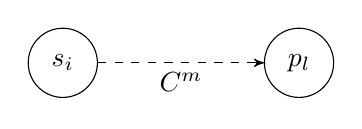
\begin{tikzpicture}[baseline=(si).base]
\node[state] (si) {$s_i$};
\node[state,right of=si] (pl) {$p_l$};
\draw
(si) edge[dashed] node[below]{$C^m$} (pl)
;
\end{tikzpicture}
\end{itemize}

\begin{korolar}
Neka je $P$ RAM-program, i označimo $n:=n_P$, $m:=u_{P^1}$. Označimo s $f:=\kf{\kprog P}^1$ jednomjesnu funkciju koju $P$ računa. Tada postoji fragment Turingovog stroja takav da za sve $k\in\N$, za sve $x\in\dom f$ prevodi reprezentaciju ($Turing_{kmn}$) početne konfiguracije s ulazom $x$ u reprezentaciju odgovarajuće završne konfiguracije, a za sve $x\in{\dom f}\kompl$, počevši od reprezentacije početne konfiguracije s ulazom $x$ nikada ne stigne u stanje $s_n$.
\end{korolar}
\begin{proof}
Samo treba spojiti sve napravljeno u ovoj točki. Nakon toga, za svaki $x\in\N$, označimo sa $(c_l)_l$ $P$-izračunavanje s $x$, i indukcijom po $l$ dokažimo da tako sastavljeni fragment Turingovog stroja dostigne konfiguraciju $Turing_{kmn}(c_l)$. Baza je upravo primjena leme~\ref{lm:pi>si} (za $i=0$) na konfiguraciju koju smo dobili iz leme~\ref{lm:faza2}. Korak je upravo primjena propozicije~\ref{prop:gadgets}. Dakle, ako $P$-izračunavanje stane u $l_0$ koraka, doći će u stanje $s_n$, u reprezentaciji završne konfiguracije $c_{l_0}$.

No vrijedi i obrat: u simulaciji jednog RAM-prijelaza $c\leadsto d$, naš fragment posjećuje samo stanja $p_i$, $s_i$ i $t_i$ za $i=c(\textsc{pc})$ ili za $i=d(\textsc{pc})$. Dakle, jedini način da dođe u stanje $s_n$ je da doista neka RAM-konfiguracija u izračunavanju preslika \textsc{pc} u $n$, a to znači da $P$-izračunavanje s $x$ stane.
\end{proof}

\begin{korolar}
Dosad izgrađeni Turingov stroj dostigne stanje $s_n$ ako i samo ako je pokrenut s ulazom $w\in\dom{\varphi_0}$, i u tom trenutku na traci nakon $\t\#$ u tragu $0$ piše $\textup\textbullet^y\textup\textopenbullet\dotsm$, gdje je $y=\N\varphi_0(\kr w)=\kr{\varphi_0(w)}$.
\end{korolar}
\begin{proof}
Samo treba primijeniti upravo dokazani korolar na RAM-program $P_0$ (dakle $f=\N\varphi_0$), na $x:=\kr w$ i $k:=\left|w\right|$. Štoviše, jer se $f$ računa na $x$ koji jest kod, dovoljno je zahtijevati $f\approx\N\varphi_0$.
\end{proof}

\begin{napomena}
Ostatak Turingovog stroja koji konstruiramo vezat će se s dosad izgrađenim dijelom isključivo kroz stanje $s_n$, i njegovo računanje će uvijek stati, pa ćemo na kraju moći zaključiti da čitav Turingov stroj stane ako i samo ako dođe u stanje $s_n$, odnosno ako i samo ako je ulazna riječ u domeni od $\varphi_0$.
\end{napomena}

Time smo riješili pitanje domene, i potrebno je još samo natrag dekodirati $y$ (ako postoji) u $\varphi_0(w)$, i postaviti ga na početak trake.

\subsection{Dekodiranje izlazne vrijednosti}

Ovaj će postupak biti vrlo sličan onome u točki~\ref{sec:tmfaza2}, samo u obrnutom smjeru. Imamo broj $y$ unarno zapisan u tragu $0$, i trebamo ga "pretvoriti u bazu $b'$" --- skidajući po jedan \textbullet\ iz traga $0$ i inkrementirajući riječ iz $\Sigma_0^*$ svaki put. Ipak, nekoliko tehničkih detalja čine ovaj postupak kompliciranijim.

Prvo, umjesto pisanja konstantnog znaka $r_1\in C^m$, morat ćemo čitati bilo koji znak koji u tragu $0$ ima \textbullet. Srećom, tehniku za to smo napravili (definicija~\ref{def:trag}).

Drugo i važnije, kod dekrementiranja smo znali da riječ neće postati dulja, te smo "nulama" \t/ skraćivali broj koliko je već potrebno, dok ga nismo dekrementirali sasvim do nule. Kod inkrementiranja nemamo tu garanciju, i općenito se može dogoditi da puno puta moramo dodati po jednu znamenku slijeva (recimo, dekadski, kad inkrementiramo $999$ u $1000$).

Zato je dobro riječ graditi unatrag, samo moramo biti sigurni da smo zauzeli dovoljno trake za to (da ne udarimo u lijevi rub, odnosno graničnik \t\$, prilikom dodavanja nove znamenke slijeva). Posljedica toga je da ne možemo učiniti intuitivno očitu stvar i upotrijebiti samo dio trake lijevo od separatora \t\#\ --- naravno, jer je taj dio ograničen duljinom ulazne riječi, a izlazna riječ može biti puno dulja od ulazne.

Spasit ćemo se tako što ćemo za rekonstrukciju izlazne riječi upotrijebiti dio desno od separatora, unutar kojeg smo simulirali $P_0$-izračunavanje s $w$. Taj dio će sigurno biti dovoljno dugačak, jer sadrži bar $y=\kr{\varphi_0(w)}$ znakova \textbullet\ u tragu $0$.

\begin{lema}
Za svaku riječ $u$ vrijedi $\left|u\right|\le\kr u$.
\end{lema}
\begin{proof}
Ako je $u=\varepsilon$, tada jednakost glasi $0\le 0$. Inače, neka je $\Sigma$ abeceda nad kojom je $u$, te $b'=1+\card\Sigma\ge2$ njena baza. Tada je kod prvog znaka od $u$ (označimo ga s $d_1$) sigurno u slici kodiranja $\N\Sigma$, dakle $d_1\ge 1$. To znači da je
\begin{equation}
    \kr u=d_1\cdot (b')^{\left|u\right|-1}\ge1\cdot2^{\left|u\right|-1}>\left|u\right|-1\text,
\end{equation}
iz čega slijedi tvrdnja jer su $\kr u$ i $\left|u\right|$ prirodni brojevi.
\end{proof}

Štoviše, taj rezultat pokazuje da riječ možemo dekodirati korak po korak: u svakom trenutku će nam u tragu $0$ ostati $y'$ znakova \textbullet, a od desnog kraja će biti napisana riječ $u'$ čiji je kod $\kr{u'}=y-y'$, pa će sigurno stati u prostor od $y-y'$ ćelija.

%\part{Posljedice univerzalnosti}
%\chapter{Teorem o parametru}
\appendix
\printbibliography

\end{document}
